\documentclass[oneside]{ctexbook}

% ============================================================
% CoreLoop 数据结构 —— 书籍级排版基础配置
% 编译方式：XeLaTeX（需要启用 shell-escape）
% 例如：latexmk -xelatex -shell-escape main.tex
% ============================================================

% ---------- 基础 ----------
\usepackage{emptypage}
\usepackage{enumitem}
\usepackage{environ}
\usepackage{graphicx}
\usepackage{booktabs}
\usepackage{tabularx}
\usepackage{array}
\usepackage{amsmath,amssymb}
\usepackage{microtype}
\usepackage[most]{tcolorbox}
\usepackage{minted}
\usepackage{tikz}
\usetikzlibrary{trees}
\usetikzlibrary{positioning}
\usepackage{hyperref}
\usepackage{textcomp}
\usepackage{circledsteps}
\usepackage{caption}
\captionsetup[figure]{
    labelsep=space
}

% 通过\uline, \uwave为文字添加下划线、下波浪线
\usepackage[normalem]{ulem}

% tcolorbox 的 minted 支持
\tcbuselibrary{minted,skins,breakable}

% ---------- 字体 ----------
% ctex 会自动处理中文字体。
% 这里显式指定一个常见的 CJK 字体，便于跨机器时理解配置。
% 如果你的 Windows 上没有 Noto Serif CJK SC，可删除这两行，让 ctex 自动选择。
% \setCJKmainfont{Noto Serif CJK SC}
% \setCJKsansfont{Noto Sans CJK SC}

% ---------- 页面 ----------
\usepackage[a4paper,margin=2.4cm,headheight=15pt]{geometry}

% ---------- 颜色 ----------
% 正文与代码都尽量克制，不做成 IDE 风格。
\definecolor{codebg}{RGB}{248,248,248}
\definecolor{codeborder}{RGB}{218,218,218}
\definecolor{codelinenum}{RGB}{125,135,145}
\definecolor{codekeyword}{RGB}{35,90,155}
\definecolor{codestring}{RGB}{45,135,85}
\definecolor{codecomment}{RGB}{110,110,110}

% 定义块：偏蓝
\definecolor{defbg}{RGB}{244,248,253}
\definecolor{defborder}{RGB}{120,160,205}
\definecolor{deftitle}{RGB}{35,90,145}

% 思考块：偏暖黄
\definecolor{thinkbg}{RGB}{253,249,238}
\definecolor{thinkborder}{RGB}{205,175,95}
\definecolor{thinktitle}{RGB}{145,105,30}

% 普通提示块：偏灰绿
\definecolor{notebg}{RGB}{246,249,247}
\definecolor{noteborder}{RGB}{145,175,155}
\definecolor{notetitle}{RGB}{55,105,70}

% 直觉解释块
\definecolor{intuitionbg}{RGB}{248,248,248}
\definecolor{intuitionline}{RGB}{90,90,90}
\definecolor{intuitiontext}{RGB}{50,50,50}

% ============================================================
% 概念展示块
% ============================================================
\definecolor{bulkbg}{RGB}{248,248,248}
\definecolor{bulkborder}{RGB}{220,220,220}

% \newcommand{} 表示创建一个新的latex命令, {}里面的\term就是创建的新命令。定义后，后面就可以使用：\term{数据结构}，\term{线性表}等。
% [1]表示这个命令接受一个参数。#1表示第一个参数的内容。如：\term{数据结构}，则#1会被替换为“数据结构”。
% \textbf{}这是latex的粗体命令，如：\texbf{数据结构}，编译后就会输出粗体的“数据结构”这几个字。
\newcommand{\term}[1]{\textbf{#1}}

\newcommand{\figref}[1]{%
    \hyperref[#1]{图~\ref*{#1}（第~\pageref*{#1}~页）}%
}

\newcommand{\coderef}[1]{%
    \hyperref[#1]{代码~\ref*{#1}（第~\pageref*{#1}~页）}%
}

% ---------- 超链接 ----------
\hypersetup{
    colorlinks=true,
    linkcolor=deftitle,
    urlcolor=deftitle,
    citecolor=deftitle,
    pdftitle={数据结构},
    pdfauthor={CoreLoop}
}

% 行号样式
\renewcommand{\theFancyVerbLine}{%
    \scriptsize\color{codelinenum}\arabic{FancyVerbLine}%
}

% 定义一个名为 cppcode 的新环境。
%
% 以后可以这样使用：
%
% \begin{cppcode}
% int main() {
%     return 0;
% }
% \end{cppcode}
% 这个环境由 tcolorbox 提供外层盒子，
% 内部使用 minted 负责 C++ 代码的排版和语法高亮。
% 使用 minted，因此中文字符串可以直接写。
\newtcblisting{cppcode}{
    enhanced,
    breakable,      % 允许代码框跨页
    listing engine=minted,  % 指定代码的排版引擎使用minted
    minted language=cpp,    % 指定 minted 使用 C++ 语言进行语法高亮。
    % minted参数 
    minted options={
        fontsize=\small,    % 设置代码字体大小，\small为比正文略小
        fontfamily=DejaVu Sans Mono,
        baselinestretch=1.15,   % % 设置代码行距相对于正常行距的倍率。
        linenos,    % 显示代码行号。
        numbersep=7pt,     % % 设置“行号”和“代码正文”之间的距离。
        breaklines,     % 当一行代码太长时，允许自动换行。
        autogobble,
        tabsize=4,   % 设置 Tab 字符对应的空格宽度。tabsize=4 表示一个 Tab 按 4 个空格的宽度排版。
        escapeinside=@@
    },
    colback=codebg,     % 设置代码框内部的背景颜色。
    colframe=codeborder,    % 设置代码框边框的颜色。
    boxrule=0.55pt,     % 设置代码框边框线的粗细。
    arc=2pt,    % 设置代码框四个角的圆角半径。
    left=15pt,   % 左侧页边距，即左侧边框与代码内容之间的空白距离。
    right=7pt,
    top=7pt,
    bottom=7pt,
    listing only,
    before skip=1em,
    after skip=1em
}

% ============================================================
% 带高亮的 C++ 代码块
% ============================================================
\NewTCBListing{cppcodeHighlight}{ O{} }{
    enhanced,
    breakable,
    listing engine=minted,
    minted language=cpp,
    minted options={
        fontsize=\small,
        fontfamily=DejaVu Sans Mono,
        baselinestretch=1.15,
        linenos,
        numbersep=7pt,
        breaklines,
        autogobble,
        tabsize=4,
        escapeinside=@@
    },
    % 这里不要写进 minted options
    % 而是通过 minted options app 追加
    minted options app/.expanded={
        highlightlines={#1},
        highlightcolor=yellow!20
    },
    colback=codebg,
    colframe=codeborder,
    boxrule=0.55pt,
    arc=2pt,
    left=15pt,
    right=7pt,
    top=7pt,
    bottom=7pt,
    listing only,
    before skip=1em,
    after skip=1em
}

% ============================================================
% 带编号的 C++ 代码块
% ============================================================
% 不显示行号：在[]里加一个参数：showlinenumber=false
\tcbset{
    codetitle/.store in=\cppcodetitle,
    showlinenumber/.is choice,
    showlinenumber/true/.code={
        \def\cpp@linenos{linenos}
    },
    showlinenumber/false/.code={
        \def\cpp@linenos{}
    }
}
\newtcblisting[
    auto counter,
    number within=chapter
]{cppcodeNum}[1][]{
    % ---------- 默认值 ----------
    codetitle={},
    showlinenumber=true,
    % ---------- 用户参数 ----------
    #1,
    enhanced,
    breakable,
    listing engine=minted,
    minted language=cpp,
    minted options={
        fontsize=\small,
        fontfamily=DejaVu Sans Mono,
        baselinestretch=1.15,
        \cpp@linenos,
        numbersep=7pt,
        breaklines,
        autogobble,
        tabsize=4
    },
    colback=codebg,
    colframe=codeborder,
    boxrule=0.55pt,
    arc=2pt,
    left=15pt,
    right=7pt,
    top=15pt,
    bottom=7pt,
    listing only,
    before skip=1em,
    after skip=1em,
    % ---------- 代码标题 ----------
    title={
        代码~\thetcbcounter
        \ifstrempty{\cppcodetitle}
            {}
            {\quad \cppcodetitle}
    },
    fonttitle=\bfseries\normalsize,
    coltitle=codekeyword,
    attach boxed title to top left={
        xshift=10pt,
        yshift=-\tcboxedtitleheight/2
    },
    boxed title style={
        colback=codebg,
        colframe=codeborder,
        boxrule=0.55pt,
        arc=2pt,
        left=6pt,
        right=6pt,
        top=2pt,
        bottom=2pt
    }
}

% ============================================================
% 定义块
% 用法：
% \begin{definitionbox}{数组}
%   ...
% \end{definitionbox}
% ============================================================
\newtcolorbox{definitionbox}{
    enhanced,
    breakable,      % 允许盒子跨页。如果定义内容很多，不会被强制挤在一页。
    colback=defbg,  % 盒子内部背景颜色。
    colframe=defborder, % 盒子边框颜色。
    boxrule=0.7pt,  % 边框线宽。
    arc=2pt,    % 圆角半径。
    left=11pt,  % 内容距离左边框的距离。
    right=11pt,
    top=15pt,
    bottom=9pt,
    before skip=1em,    % 盒子与前面正文之间的距离。
    after skip=1em,     % 盒子与后面正文之间的距离。
    title={定义},       % 设置标题文字。
    fonttitle=\bfseries\large,  % 标题字体样式。\bfseries表示加粗，\Large表示某个字体大小（大号字体）。
    coltitle=deftitle,  % 标题文字颜色
    % 将标题框（定义二字所在的框）移动到主框左上角。
    %
    % xshift:
    %   水平方向移动
    %
    % yshift:
    %   垂直方向移动
    %
    % \tcboxedtitleheight:
    %   自动获取标题框高度。
    attach boxed title to top left={xshift=10pt,yshift=-\tcboxedtitleheight/2},
    boxed title style={
        colback=defbg,          % 标题小框背景色。
        colframe=defborder,     % 标题小框边框颜色。
        boxrule=0.7pt,          % 标题小框边框粗细。
        arc=2pt,                % 标题小框圆角。
        left=6pt,               % 标题文字距离左边框。
        right=6pt,              % 标题文字距离右边框。
        top=1pt,
        bottom=1pt
    }
}

% ============================================================
% 直觉解释块
%
% 用法：
%
% \begin{intuitionbox}
% 数据结构，就是我们研究和处理的一个个“东西”。
% \end{intuitionbox}
%
% ============================================================

\newtcolorbox{intuitionbox}{
    enhanced,
    breakable,
    colback=intuitionbg,
    frame hidden,
    borderline west={3pt}{0pt}{intuitionline},
    left=12pt,
    right=12pt,
    top=8pt,
    bottom=8pt,
    before skip=1em,
    after skip=1em,
    fontupper=\small,
    colupper=intuitiontext
}

% ============================================================
% 思考块
% 用法：
% \begin{thinkbox}{想一想}
%   ...
% \end{thinkbox}
% ============================================================
\newtcolorbox{thinkbox}{
    enhanced,
    breakable,
    colback=thinkbg,
    colframe=thinkborder,
    boxrule=0.7pt,
    arc=2pt,
    left=7pt,
    right=7pt,
    top=10pt,
    bottom=6pt,
    before skip=1em,
    after skip=1em,
    title={思考},
    fonttitle=\bfseries\normalsize,
    coltitle=thinktitle,
    attach boxed title to top left={xshift=10pt,yshift=-\tcboxedtitleheight/2},
    boxed title style={
        colback=thinkbg,
        colframe=thinkborder,
        boxrule=0.7pt,
        arc=2pt,
        left=4pt,
        right=4pt,
        top=0pt,
        bottom=0pt
    }
}

% ============================================================
% 思维拓展块 Insight
% ============================================================
\definecolor{insightbg}{RGB}{246,246,252}
\definecolor{insightborder}{RGB}{140,140,190}
\definecolor{insighttitle}{RGB}{80,80,150}

\newtcolorbox{insightbox}{
    enhanced,
    breakable,
    colback=insightbg,
    colframe=insightborder,
    boxrule=0.7pt,
    arc=2pt,
    left=7pt,
    right=7pt,
    top=11pt,
    bottom=6pt,
    before skip=1em,
    after skip=1em,
    title={*思维拓展},
    fonttitle=\bfseries\normalsize,
    fontupper=\small,
    coltitle=insighttitle,
    attach boxed title to top left={
        xshift=10pt,
        yshift=-\tcboxedtitleheight/2
    },
    boxed title style={
        colback=insightbg,
        colframe=insightborder,
        boxrule=0.7pt,
        arc=2pt,
        left=5pt,
        right=5pt,
        top=0pt,
        bottom=0pt
    }
}

% ============================================================
% 普通提示块（额外给你一个可选样式）
% ============================================================
\newtcolorbox{notebox}[1]{
    enhanced,
    breakable,
    colback=notebg,
    colframe=noteborder,
    boxrule=0.6pt,
    arc=2pt,
    left=12pt,
    right=12pt,
    top=9pt,
    bottom=9pt,
    before skip=1em,
    after skip=1em,
    title={#1},
    fonttitle=\bfseries,
    coltitle=notetitle,
    boxed title style={
        colback=notebg,
        colframe=noteborder,
        boxrule=0.6pt,
        arc=2pt
    }
}

% ============================================================
% 概念展示块
%
% 用法：
%
% \begin{bulk}
% 节点A → 节点B → 节点C
% \end{bulk}
%
% ============================================================
\newtcolorbox{bulk}{
    enhanced,
    breakable,
    colback=bulkbg,
    colframe=bulkborder,
    boxrule=0.6pt,
    arc=8pt,
    left=10pt,
    right=10pt,
    top=7pt,
    bottom=7pt,
    before skip=1em,
    after skip=1em,
    fontupper=\small
}

% ============================================================
% 书签 / 内容跳转标记
% 用法：
%
% \bookmark{label}{标题}
%
% 例如：
% \bookmark{bookmark:array}{顺序表的实现}
%
% 引用：
%
% \bookmarkref{bookmark:array}{顺序表的实现}
%
% 效果：
% ─────────── 顺序表的实现 ───────────
%
% 如果已经看懂了，请直接跳至【顺序表的实现】处（第 15 页）。
% ============================================================
\newcommand{\bookmark}[2]{%
    \par
    \medskip
    \noindent
    \makebox[\textwidth]{%
        \leaders\hrule height 0.5pt\hfill
        \quad
        \textbf{#2}
        \quad
        \leaders\hrule height 0.5pt\hfill
    }%
    \label{#1}%
    \par
    \medskip
}

\newcommand{\bookmarkref}[2]{%
    \hyperref[#1]{---#2---}（第~\pageref{#1}~页）%
}

% 有序列表编号。使用方式：
% \minisection{1. 顺序存储}
% 这里介绍顺序存储……
% \minisection{2. 链式存储}
% 这里介绍链式存储……
\newcommand{\minisection}[1]{%
    \par\medskip
    \noindent\textbf{#1}
    \par\smallskip
}

% =========================================================
% 习题与习题答案
% =========================================================

% ---------------------------------------------------------
% xsim
%
% use-files：
% 将习题和答案正文写入外部 .tex 文件，
% 因此可以安全使用 minted / verbatim。
%
% blank：
% 不使用 xsim 默认的 exercise / solution 环境，
% 我们自己定义 exercise / exerciseanswer。
% ---------------------------------------------------------

\usepackage[use-files,blank]{xsim}
% =========================================================
% 定义习题类型
% =========================================================
\DeclareExerciseType{bookexercise}{
    exercise-env      = exercise,
    solution-env      = exerciseanswer,
    exercise-name     = 习题,
    exercises-name    = 习题,
    solution-name     = 习题参考答案,
    solutions-name    = 习题参考答案,
    exercise-template = book-exercise,
    solution-template = book-solution,
    exercise-heading  = \subsection*,
    solution-heading  = \subsection*
}

% =========================================================
% 习题环境模板
% =========================================================
\DeclareExerciseEnvironmentTemplate{book-exercise}{
    \par
    \medskip
    \noindent
    \textbf{习题 \GetExerciseProperty{counter}}%
    \quad
    \IfExistSolutionTF{
        （参考答案见习题
        \GetExerciseProperty{counter}~参考答案，第
        \pageref{exercise-answer:\ExerciseID}页）
    }{}
    \par
    \medskip
    \label{exercise:\ExerciseID}
}{
    \par
    \medskip
}


% =========================================================
% 习题答案环境模板
% =========================================================

\DeclareExerciseEnvironmentTemplate{book-solution}{
    \clearpage
    \phantomsection
    \label{exercise-answer:\ExerciseID}
    \noindent
    \textbf{习题 \GetExerciseProperty{counter}~参考答案}
    \par
    \medskip
}{
    \par
    \medskip
}


% =========================================================
% xsim 设置
% =========================================================

\xsimsetup{
    exercise/print = true,
    print-solutions/headings = false
}


% =========================================================
% 打印所有习题答案
% =========================================================

\newcommand{\printanswers}{%
    \clearpage
    \chapter*{习题参考答案}
    \addcontentsline{toc}{chapter}{习题参考答案}
    \markboth{习题参考答案}{习题参考答案}
    \printsolutionstype[
        headings = false
    ]{bookexercise}%
}

% ============================================================
% 树结构节点样式
% ============================================================
\tikzset{
    treenode/.style={
        font=\small,
        align=center,
        inner sep=2pt
    }
}

% ============================================================
% 图结构节点样式
% ============================================================

\tikzset{
    graphnode/.style={
        font=\small,
        inner sep=2pt
    }
}

% ============================================================
% 图片与表格的默认设置
% ============================================================
\setlength{\tabcolsep}{7pt}
\renewcommand{\arraystretch}{1.25}

\newcommand{\bookfigure}[4]{%
    \begin{figure}[htbp]
        \centering
        \includegraphics[width=#2\textwidth]{#1}
        \caption{#3}
        \label{#4}
    \end{figure}%
}

% ============================================================
% 文档信息
% ============================================================
\title{前有数据结构}
\author{CoreLoop}
\date{}
\renewcommand{\contentsname}{地\;\;图}
\begin{document}

\maketitle

\frontmatter

\chapter*{UNKNOWN VOICE}
是的，没错，这片大陆叫做《数据结构》，是历代先贤们以智慧为剑刃开辟的疆土，也是无数求知者在0与1的荒原上寻找真理的朝圣之地。寻理者皆向北而行，并了解了
逻辑的含义。\\


位不见王影，然火焰映彻苍穹。当传承火焰燃烧之时，钟声将响彻四周，进而唤醒遍布这片大陆的思渡者们。\\

幽邃圣者 栈和队列， 深渊监视者，树与二叉树，以及罪业之都的孤独王者 -- 图。不过啊，王者们一定会筑起不可逾越的高墙吧。而无火的余灰将会纷至踏来，那是无名、成不了薪，
被命运牵绊的思渡者。但也正因如此，灰烬才会如此渴求余火吧。\\\\\\


落叶捎来消息：在雾的彼端，我们的故乡“交界地”，那伟大的艾尔登法环已经破碎，“永恒女王”玛莉卡销声匿迹，在黑刀阴谋之夜，“黄金”葛德文最先失去性命，玛莉卡之子 -- 
诸位半神拿到艾尔登法环的碎片。却因为那股力量堕入歧途、陷入疯狂、引发碎片战争...... 
在那场无王存在的战争最后 -- 无上意志放逐了他们。奥，所以啊，褪色者啊 -- 依旧无法永眠的死者啊，那许久以前我们失去的赐福，正在出声呼唤。
“蛮荒地王者” 荷莱 露。 光耀金面具、“死眠少女”菲雅、受尽唾弃的食粪者、“百智爵士”基甸 奥夫尼尔。
...... 那失去的赐福又再一次，回到默默无名的褪色者身上。朝雾的彼端前进，抵达交界地，觐见艾尔登法环 -- 成为艾尔登之王吧。



\chapter*{--------- BONFIRE HIT ---------}
欢迎来到营火，无火的余灰大人。我正是营火的维护者，专门维护营火以及服侍您的人。\\

这里就是数据结构大陆中不显眼的一角------《前有数据结构》，这片大陆的守护神亦是开创者，大家都称其为CoreLoop。如果您为了觐见\term{树、图}等王者们而需要帮助，我很愿意为此帮忙。\\

首先，CoreLoop托我带给您以下谏言，愿它们能照亮您前行的路。
\begin{enumerate}
    \item 《前有数据结构》假设您已经有了比较好的C语言基础，但他也会在某些合适的地方强调某些C语言的知识点。
    \item 在您思渡的过程中，遇到的所有“思维拓展”\textbf{都 ！可！以！完！全！跳！过！!} 我向您保证，即使跳过这些，您也决不会错过与《数据结构》本身无关的内容。
\end{enumerate}

如果你对本书中的内容存在疑问，欢迎联系作者。【联系方式】

许多地方添加一些内容，能够对正文有很好的补充及/或帮助大家理解的作用，但是为了保证在本书中不过分多地引入与《数据结构》本身无关的内容，作者并未给出这些“DLC”。
如果想要了解，请参考我的视频。




知识绝不会少，但更重要的是思考。

很多有意思的东西都是藏在习题里面。

即使引导早已破碎，也请您成为数据结构之王。

恭喜你找到了第一个篝火。你可以在此处整理背包，回忆这段旅程的所见所闻，并且将所得卢恩转化为力量，并解锁一些新的能力。后续可以在适合的篝火处和读者说说话。



继续向前，便是CoreLoop所开创的大陆。我将不离不弃地伴您同行，直至旅途的终点。首先，请您收下这份地图。

\tableofcontents

\mainmatter

\chapter{数据结构}
\bookmark{bookmark:mark-1}{mark-1}
欢迎来到我的大陆。请您放心，我不会在此处引入诸如“数据”的定义、什么是“数据结构三要素”等等内容。但是
同时也请您放心，我会让您彻底搞懂，什么是“数据结构”，“数据结构”究竟是在研究什么。% Latex中，通过\\ 另起一行。

\section{数据结构}
\label{sec:数据结构}
事实上，“数据结构”看起来抽象晦涩的定义，恰恰能够最好地理解“什么是数据结构”。接下来就请你随我一起进入这段拨云见日的旅程。
\begin{definitionbox}
    \term{数据结构}是相互之间存在一种或多种特定“关系”的数据元素的集合，以及定义在这些数据元素上的“操作”的集合。
\end{definitionbox}
我们以一个例子开启这段旅程：假设你是一个游戏程序员，你要编写一个游戏，玩家操控具有四个“角色”组成的小队，如：邪念、银心、
甘尔以及张三这四个人，那么，每个“角色”就都可以被看成是一个数据元素。
\begin{intuitionbox}
\textbf{数据元素}，就是我们要研究和处理的一个个“东西”。这些“东西”可以是一个游戏角色、一件装备、一条聊天消息、
一个整数、甚至一张地图等等。
\end{intuitionbox}
但是，仅仅有了四个数据元素，还不能叫“数据结构”，我们还要解决一个问题：这四个人是什么关系？比如你设计的游戏玩法是将
四人排成一个有前后顺序的队伍，那么四人便会有如下的\uwave{线性关系}：
\begin{bulk}
\begin{center}
邪念 → 银心 → 甘尔 → 张三
\end{center}
\end{bulk}
或者你设计的玩法是一个队长三个队员，则四个人便有如下的\uwave{树状关系}：
\begin{bulk}
\begin{center}
\begin{tikzpicture}
[
    level distance=1.2cm,
    sibling distance=2cm
]
\node[treenode]{邪念}
    child {
        node[treenode]{银心}
    }
    child {
        node[treenode]{甘尔}
    }
    child {
        node[treenode]{张三}
    };
\end{tikzpicture}
\end{center}
\end{bulk}
再假设，四个人之间互相存在好感度，则四个人可能有如下的\uwave{图结构}：
\begin{bulk}
\begin{center}
\begin{tikzpicture}
% 节点
\node[graphnode] (A) {邪念};
\node[graphnode] (B) [right=2cm of A] {银心};
\node[graphnode] (C) [below=1.5cm of A] {甘尔};
\node[graphnode] (D) [below=1.5cm of B] {张三};

% 边 + 权值
\draw (A) -- node[above] {5} (B);
\draw (A) -- node[left] {2} (C);
\draw (A) -- node[right] {8} (D);
\draw (B) -- node[right] {3} (D);
\draw (C) -- node[below] {6} (D);
\end{tikzpicture}
\end{center}
\end{bulk}
请注意，这里我们使用\uwave{无向图}描述，是因为我们假设了A对B的好感度与B对A的好感度相同，但现实中往往并非如此，要描述这种更
现实的情况，就要使用{\color{red}\textbf{后面将会介绍到的}}\uwave{有向图}。

到现在，“数据结构”这个词是不是已经变得具体了？再回看数据结构的定义，我们看到它还有后半句：“操作”。

假设现在我们的游戏队伍：
\begin{bulk}
\begin{center}
邪念 → 银心 → 甘尔 → 张三
\end{center}
\end{bulk}
玩家可能会在游戏中让某些人“加入队伍”（Insert），某些人“退出队伍”（Delete），如卡姐加入：
\begin{bulk}
\begin{center}
邪念 → 银心 → 甘尔 → 张三 → 卡姐
\end{center}
\end{bulk}
邪念退出：
\begin{bulk}
\begin{center}
银心 → 甘尔 → 张三 → 卡姐
\end{center}
\end{bulk}
这里“入队”、“出队”，就都是所谓的“定义在这些数据元素上的操作”。再比如，
新人入队前，你可能需要判断当前队伍是否已满，因此需要“获取队伍人数”（GetSize），这也是“定义在这些数据元素上的操作”。

有了以上的介绍，再回过头来看那个之前觉得它晦涩难懂的数据结构定义，就豁然开朗了。

任何一本《数据结构》的教材，都一定会有“线性表”、“队列”、“树”、“图”等这些内容。为什么我们要重点研究这些数据结构呢？
经过简单的思考不难发现，“线性表”、“队列”、“树”、“图”等，正是我们处理实际需求时，组织数据所需要的最有用的、最常见的结构。
比如，一个有趣的事实是：你的个人计算机中目录结构的组织，其实就是一棵树。如：
\begin{bulk}
\begin{center}
\begin{tikzpicture}
[
    level distance=1.2cm,
    level 1/.style={
        sibling distance=6cm
    },
    level 2/.style={
        sibling distance=1.8cm
    },
    level 3/.style={
        sibling distance=1.5cm
    },
]
\node[treenode]{此电脑}
    child {
        node[treenode]{本地磁盘(C:)}
        child{
            node[treenode]{Program Files}
        }
        child{
            node[treenode]{Windows}
        }
        child{
            node[treenode]{用户}
        }
        child {
            node[treenode]{...}
        }
    }
    child {
        node[treenode]{新加卷(D:)}
        child{
            node[treenode]{电影}
            child {
                node[treenode]{泰坦尼克号}
            }
            child {
                node[treenode]{...}
            }
        }
        child{
            node[treenode]{照片}
        }
        child {
            node[treenode]{...}
        }
    };
\end{tikzpicture}
\end{center}
\end{bulk}
请注意，以上出现的线性结构、树状结构、图结构，都只是逻辑意义上的结构，展示出数据元素之间的逻辑关系，而非数据元素物理存储（如在主存或磁盘中）的位
置关系。这种逻辑上的关系称为数据的\term{逻辑结构}。《数据结构》不仅研究数据的逻辑结构，还要研究如何实现物理存储，这通常通过计算机语言来实现。本书中后面
我们介绍到的每一种数据结构，都会给出其比较常见的、一般的实现方式。如果你感兴趣的话可以想一想，以上出现的数据结构，你如何通过你已有的编程语言知识来实现？

\section{算法与算法效率的度量}
我们已经知道，数据结构研究的是数据的组织方式以及对这些数据的操作。事实上，同样的一批数据，由于组织方式不同，
可能会导致操作效率产生巨大的差异。因此，在实际程序中，我们在考虑数据应该如何组织的同时，也要考虑面对
这些数据，我们应该采用什么步骤和方法去解决问题？例如：
\begin{itemize}[itemsep=0pt,
    parsep=0pt,
    topsep=0pt]
    \item 如何在一组数据中快速找到目标元素？
    \item 如何将一组无序数据排列成有序序列？
    \item 如何在复杂的网络关系中寻找最短路径？
\end{itemize}

对于同一个问题，往往存在多种不同的\uwave{算法}。它们可能都能得到正确结果，但执行过程中的时间消耗、空间占用
可能存在巨大差异。一个算法的效率正是通过其“时间消耗”与“空间占用”来衡量的，正如下面将要介绍的\term{时间复杂度}和
\term{空间复杂度}。

\subsection{时间复杂度}
我们描述一个算法的时间消耗，不能简单地说出类似“算法A需要3秒，算法B需要0.001秒”这样的话。因为代码的运行时间受到
CPU性能等诸多因素的影响。因此，我们需要一种与机器无关的评价方法，这便是\term{时间复杂度}。算法的\term{时间复杂度}，
是指算法执行时间\uline{随问题规模增长而变化}的数量级关系。我们以一个最简单的，在数组中顺序查找某个元素的算法为例来说明：
\begin{cppcode}
for(int i = 0; i < n; i++)
{
    if(a[i] == x)
        return i;
}
\end{cppcode}
这里\(n\)是数组的大小，也即问题规模大小。如何描述该算法的时间复杂度？一个很准确的做法是用该算法的\term{基本操作}的次数来描述。所谓\term{基本操作}，
是指该算法中执行次数最多的、能代表性能瓶颈的操作。该例中，循环执行若干次 i<n, a[i]==x, 以及 i++ 的操作，这两个判断及一个变量自增就是该算法的基本操作。
我们使用\term{\(T(n)\)}来描述算法的基本操作次数，显然，该例中，最坏情况下查找到最后一个，算法才会返回，因此最坏情况下：
\[
T(n)=n
\]
而平均情况下：
\[
T(n) = \frac{1}{n}\cdot 1 + \frac{1}{n}\cdot 2 + ... + \frac{1}{n}\cdot n = \frac{n+1}{2}
\]
这表示若输入规模\(n\)增加一倍，则算法在最坏情况下执行次数也会增加一倍，而平均情况下，执行次数会增加\(\frac{n+1}{2}\)。这便是
时间复杂度的“大T表示法”。

而实际的学术或工程中最最常用的，也相信你一定已经见过了的，并非大T表示法，而是\term{“大O表示法”}：

考虑某算法的时间复杂度为
\[
T(n) = 3n^{2} + 5n + 10
\]
当\(n\)很大时，该算法的时间代价几乎完全由\(3n^2\)这一项决定，而后面两项可以忽略不计。而3是常数，不随问题规模\(n\)的变化而变化。因此，使用
大O表示法，我们说该算法的时间复杂度是\(O(n^2)\)。若某算法的时间复杂度不随问题规模\(n\)的变化而变化，则我们说该算法的时间复杂度为\(O(1)\)。
对于大O表示法严谨的数学定义，感兴趣的同学请自行参考相关资料。
根据我们已有的数学知识，不难得出，在问题规模\(n\)很大的情况下：
\begin{bulk}
    \(O(1)\) 优于 \(O(logn)\) 优于 \(O(n)\) 优于 \(O(nlogn)\) 优于 \(O(n^2)\) 优于 \(O(n^3)\) 优于 \(O(a^n)\)
\end{bulk}
\begin{insightbox}
这里还有一个拉扯感比较强的问题：所谓“问题规模很大”，“很大”的边界在哪？比如某个问题我们确定问题规模\(n\)一定满足\(n<=100\)，那么，
\(T(n) = n^3\), 即\(O(n) = n^3\)的算法，是不是反而优于\(T(n) = 101n^2\), 即\(O(n) = n^2\)的算法？答案是：是的。这个问题也说明了，大O复杂度
并不是算法实际运行效率的绝对比较。但是在实际的工程中，性能瓶颈通常是由大规模（n很大）的数据部分产生的，这也是实际中都在使用大O复杂度的原因。
\end{insightbox}

\subsection{空间复杂度}
某算法的\term{空间复杂度}是指实现该算法所需额外存储空间\uline{随问题规模增长而变化}的数量级关系。同时间复杂度一样，绝大多数情况下我们关注的是算法
所需额外存储空间随问题规模\(n\)的增长趋势，因此我们同样使用大O表示法来描述空间复杂度。

请注意，计算空间复杂度时我们只考虑处理问题而额外引入的空间，并不计算输入数据本身的空间。比如以下数组求和的例子，我们只引入了存储变量 i 和 result 的
两个额外 int 大小的空间，该空间大小与问题的输入规模\(n\)无关，因此该算法的空间复杂度为O(1)，而数组a[]是问题本身的数据，其存储空间并不算入空间复杂度：
\begin{cppcode}
int sum(int a[], int n)
{
    int result = 0;
    for(int i=0; i<n; i++)
    {
        result += a[i];
    }
    return result;
}
\end{cppcode}

\begin{notebox}{提示}
    分析空间复杂度很简单，只需要看程序额外使用了多少内存。如果你对时间复杂度没有“感觉”，笔者在这里给出一个建立感觉的提示。如前所述，时间复杂度要看程序
    执行次数最多、最能代表瓶颈的操作。通常来说，执行次数最多的循环就是程序的瓶颈。如：
    \begin{cppcode}
        void f(int n) { // 模拟问题的输入规模为n
            int a = 10;
            int b = a + 2;
            // 该循环约执行 n 次，复杂度为n量级
            for(int i=0; i<n; i++) {
                // ...
            }
            // 该循环约执行 n+(n-1)+...+2+1 次，复杂度为@\(n^2\)@量级
            for(int i=0; i<n; i++) {
                for(int j=i; j<n; j++) {
                    // ...
                }
            }
            // 该循环约执行 nlogn次，复杂度为nlogn量级
            for(int i=0; i<n; i++) {
                for(int j=1; j<n; j*=2) {
                    // ...
                }
            }
        }
    \end{cppcode}
    以上代码中，显然
    \begin{cppcode}
        // 该循环约执行 n+(n-1)+...+2+1 次，复杂度为@\(n^2\)@量级
        for(int i=0; i<n; i++) {
            for(int j=i; j<n; j++) {
                // ...
            }
        }
    \end{cppcode}
    为程序的性能瓶颈。因此我们说算法f的时间复杂度是\(O(n^2)\)。
\end{notebox}

\section{\color{red}\textbf{标题还没想好}}
通过以上的介绍，我们就了解了《数据结构》或者叫《数据结构与算法》这个学科，就是研究在不同的实际需求下，数据如何存储、组织，以及高效操作的学科。

任何一本数据结构的教材都会重点介绍“线性表”、“队列”、“树”、“图”等数据结构，这是因为这些结构并不是枯燥的理论模型，而是计算机世界中最常见、最高效的组织方式。
当你打开一个游戏背包，当你浏览一棵文件目录树，当你在地图中寻找一条最短路径，当你在社交网络中查看好友关系，你看到的表象虽然不同，但它们背后都隐藏着数据结构的思想。

笔者认为，《数据结构》这个学科次在“掌握知识”，而重在“培养能力”。学习《数据结构》，真正重要的是，在学习的过程中不断思考、体会和理解这些数据结构与算法背后的思想及其
代码实现原理，训练自己灵活的思维和解决问题的能力。这也是在本书中我将一遍又一遍地强调的内容。

那接下来，就我们将一起走进这段探索之旅，逐一认识这些经典结构，理解它们为什么诞生，以及它们如何帮助我们更加高效地解决实际问题。在此之前，如果你是一个喜欢思考问题的人，
不妨看看下面的“思考”。
说不定天才的你能够自己探索出最优解（甚至想出了比目前已知的最优解更优的解法，顺便发表一篇论文什么的）。以下的这些问题呢，也会随着本书后续的开展，
而不断地展开讨论，相信你每次回看它们的时候，都会有全新的不同理解。
\begin{thinkbox}{想一想}
{\color{red}\textbf{这里给出一些思考吧，学习本书之前，可以自己瞎想一下，学完本书之后，都给出一个很优的答案，尽量做到每种结构一个例子。}}
\end{thinkbox}


\begin{cppcodeNum}[label={code:test}, codetitle={测试代码}]

int main() {
    int a = 10;
    int b = 20;

    int c = a + b;

    return 0;
}

\end{cppcodeNum}

带页码：如\figref{fig:顺序存储的线性表}所示。如\coderef{code:test}所示。
不带页码：如图\ref{fig:顺序存储的线性表}所示。如代码\ref{code:test}所示。
\chapter{线性表}

欢迎来到第二章。


假设某游戏的玩法是玩家操控一个四人组成的小队，队伍成员存在严格有序的位置关系，类似这样：
\begin{bulk}
\begin{center}
邪念 → 银心 → 甘尔 → 张三
\end{center}
\end{bulk}
这，其实就是一个由四个“游戏中的可操控角色”构成的\uwave{线性表}，表中有四个元素，元素的类型是“角色”，可能类似这样：
\begin{cppcodeNum}[label={code:Role类型定义}]
struct Role{
    int hp;             // 生命值
    int attack_power;   // 攻击力
    // ...              // 其他
};
\end{cppcodeNum}
有了这个例子，我们给出如下线性表的定义：
\begin{definitionbox}
    \term{线性表}是具有\uline{相同数据类型}的\(n(n>=0)\)个元素构成的有限\uline{有序}序列，其中\(n\)为表长，当\(n=0\)时线性表是一个空表。
\end{definitionbox}
请注意，线性表所称元素“有序”，这并不是说元素的值大小有序，而是元素有严格的位置关系。例如，我们可以用\(L\)将线性表表示为：
\[
L = (a_1, a_2, ..., a_n)
\]
其中，\(a_1\)是唯一的第一个元素，\(a_n\)是唯一的最后一个元素。

\section{顺序表和链表简介}
线性表最常见的实现方式有两种。在C语言中，我们可以利用数组让这些元素在内存中连续地存放。这种利用一段连续的存储空间依次保存表中元素的线性表被称为\term{顺序表}。
顺序表的存储结构定义如代码\ref{code:线性表的顺序存储结构}所示。
\begin{cppcodeNum}[label={code:线性表的顺序存储结构}, codetitle={线性表的顺序存储结构}]
    #define MaxSize 100
    struct SeqList{  // SeqList, 即Sequential List
        ElemType data[MaxSize];  // 存放表中元素，可用数组下标为0-99
        int current_size;       // 当前表中的元素数量
    };
\end{cppcodeNum}
其对应的物理存储结构如图\ref{fig:顺序存储的线性表}所示。
\begin{figure}[htbp]
    \centering
    % trim: 左 下 右 上
    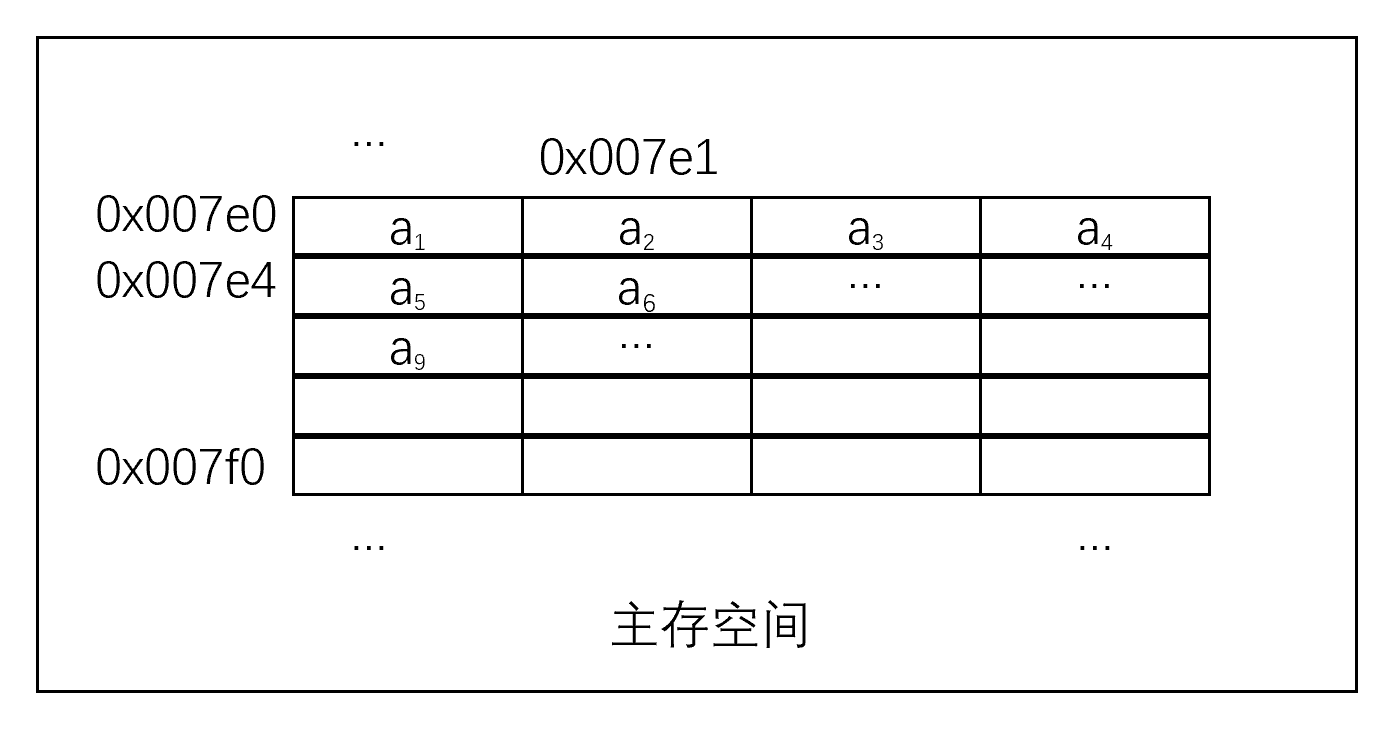
\includegraphics[width=0.55\textwidth, trim=0 1.5cm 0 0]{assets/pics_and_ppts/ch2/顺序存储的线性表.png}
    \caption{顺序存储的线性表}
    \label{fig:顺序存储的线性表}
\end{figure}

\begin{notebox}{初见提示}
相信你懂我的意思，但初见我还是要多啰嗦一句：图\ref{fig:顺序存储的线性表}中我们假设了某顺序表起始地址为0x007e0，每个元素大小为1字节。
而在后续诸多内容中我们将省去这种用于严谨的话术，而专注于“传意”的意图。
\end{notebox}

\begin{notebox}{提示}
代码\ref{code:线性表的顺序存储结构}中，我们用ElemType(Element Type)表示表中的元素类型。比如你要处理一组int型数据，把它们放在线性表中，ElemType就可以是int类型；再比如你要处理四个游戏角色，
ElemType就可以是Role类型(类似代码\ref{code:Role类型定义})。
\end{notebox}
顺序表保证了逻辑上相邻的两个元素物理上也一定相邻。因此，表中任何一个元素的地址都可以由
\begin{bulk}
    \begin{center}
        Address(\(a_i\)) = Address(\(a_1\)) + sizeof(ElemType) \(\cdot\) (\(i-1\)) 
    \end{center}
\end{bulk} 
计算得来。因此，访问（读或写）顺序表中的任意一个元素，都可以在O(1)时间内实现，这种特性我们称为\term{顺序表支持随机访问}。
\begin{insightbox}
若线性表可以对任意元素\(a_i\)进行读写，而且操作时间为\(O(1)\)，与\(i\)和数组大小\(n\)无关，则这种访问方式称
为\term{随机访问（random access）}。如何理解“随机”？第一，可以理解为表可以对任一位序实现O(1)的访问效率，即使位序是“随机”给出的。
第二，与链表做对比。我们将马上看到，链表只能顺序访问（sequential access），而无法随机访问。也就是说，要访问链表中位序为i的元素，
我们必须依次访问\(a_1\), \(a_2\), ..., \(a_{i-1}\), \(a_i\)。而无法跳过前面直接访问\(a_i\)。
\end{insightbox}
不难想到，可以使用如下代码初始化一个顺序表并为其构造元素：
\begin{cppcode}
    // 假设我们要将存放在数组a中，长度为n的数据插入某个顺序表中 
    struct SeqList L;        // 定义一个顺序表
    L.current_size = 0;     // 空表初始元素数量为0
    // 插入数据
    for(int i=0; i<n; i++) {
        if(L.current_size < MaxSize) {    
            L.data[L.current_size] = a[i];  
            L.current_size++;
        } else {
            // 表已满，拒绝插入
        }
    }
\end{cppcode}

通过C语言提供的指针，我们也可以让每个元素通过一个指针指向下一个元素，从而链接起整个线性表。这种通过指针，将一个个物理上未必连续的存储空间链接起来的
线性表被称为\term{链表}。在这种实现方式下，表的每个节点除了存储数据元素本身，还要额外存储一个“指向下一个元素的指针”。因此，我们需要一个struct来
描述表的一个“节点”：
\begin{cppcode}
    struct ListNode{
        ElemType data;  // 该节点的数据元素
        struct ListNode* next_node; // 下一个节点的地址 
    };
\end{cppcode}
\begin{figure}[htbp]
    \centering
    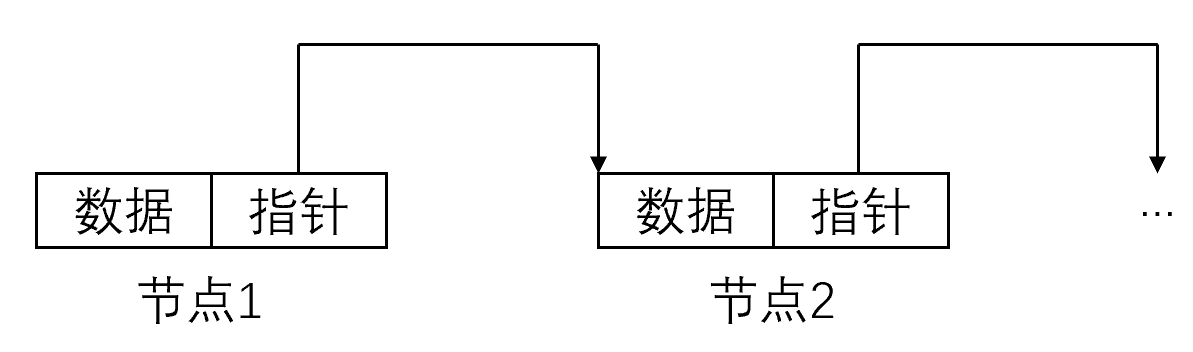
\includegraphics[width=0.5\textwidth, trim=0 1cm 0 0]{assets/pics_and_ppts/ch2/链表的节点.png}
    \caption{链表的节点}
    \label{fig:链表的节点}
\end{figure}
由于有了第一个链表节点的指针，就可以顺着链条找到所有节点，因此，一个链表可以用其第一个节点的指针来表示：我们定义
\begin{cppcode}
    typedef struct ListNode* LinkList;  // LinkList 是指向ListNode的指针类型 
\end{cppcode}
于是，就可以用
\begin{cppcode}
    LinkList L;
\end{cppcode}
来定义一个“链表”对象L（就像用"int a;"来定义一个int型对象a一样）。
\begin{notebox}{提示}
    LinkList与ListNode*是同一种类型。只不过语义上强调的重点不同：ListNode*强调“这是一个节点”，而LinkList强调“这是一个链表”。我们也经常使用
    \begin{bulk}
        typedef struct ListNode* head;
    \end{bulk}
    来突出head是链表第一个节点的指针。
\end{notebox}
链表的物理存储结构如图\ref{fig:链式存储的线性表}所示。
\begin{figure}[htbp]
    \centering
    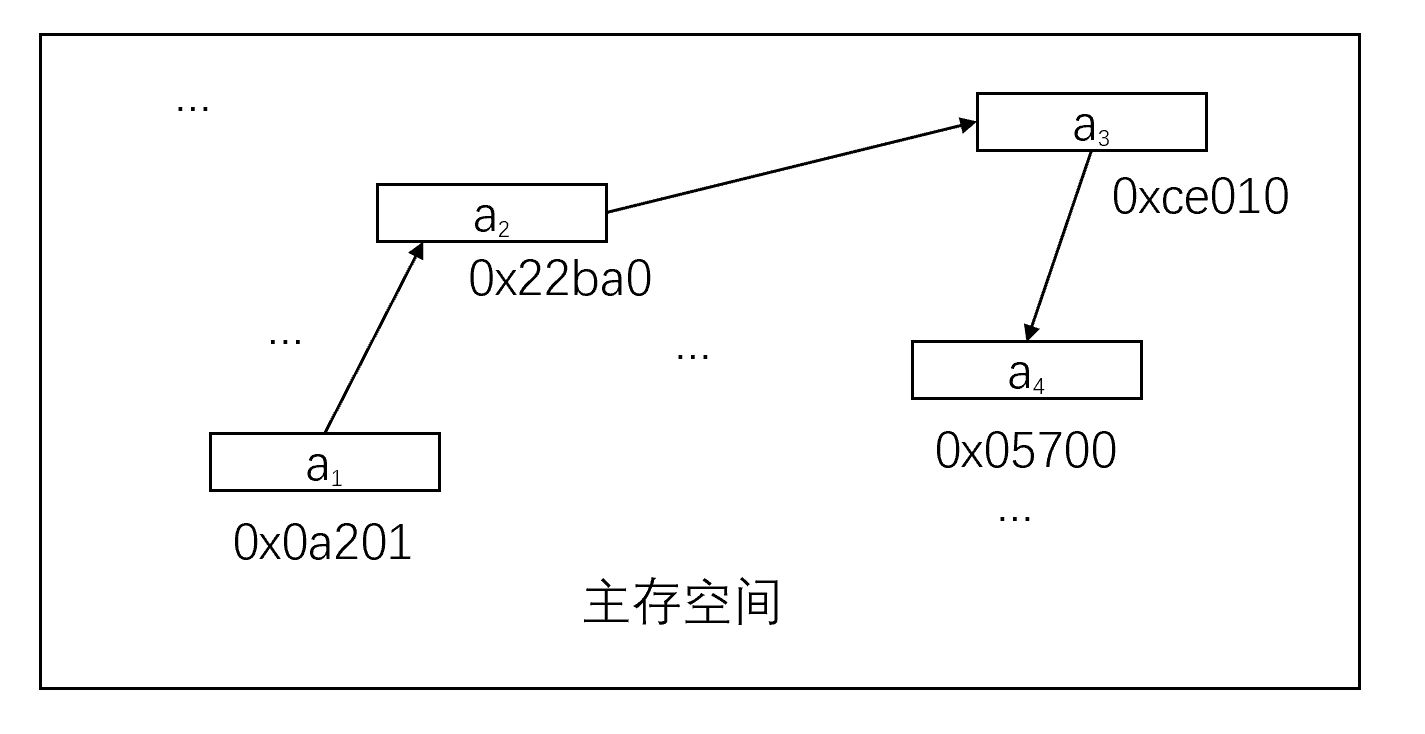
\includegraphics[width=0.55\textwidth, trim=0 1.2cm 0 0]{assets/pics_and_ppts/ch2/链式存储的线性表.png}
    \caption{链式存储的线性表}
    \label{fig:链式存储的线性表}
\end{figure}
现在假设我们要将存放在数组a中，长度为n的数据插入某个链表中，请你尝试写出C语言代码。后面我们会给出更一般化的代码。

\section{顺序表}
经过上面的介绍我们可以看出，顺序表的优点在于：\Circled{1}支持随机访问，访问表中任意元素可以O(1)时间实现；\Circled{2}几乎无需额外存储空间存储额外信息，
不像链表那样需要额外存储n个指针。顺序表的缺点也很明显：插入或删除表中元素时需要移动大量元素。

接下来我们给出顺序表常见操作的代码实现，通过代码大家也可以进一步体会这一点。对于一个未初始化的顺序表L：
\begin{cppcode}
    struct SeqList L;
\end{cppcode}
\minisection{1.顺序表的初始化操作}
顺序表中通过一个整数变量current\_size来维护当前表长（表中已有元素数量）。初始化时，将其置为0：
\begin{cppcode}
    void InitList(struct SeqList *L) {
        L->current_size = 0;
    }
\end{cppcode}
\minisection{2.顺序表的插入操作}
以下函数实现了操作：在顺序表L中，第index个位置插入一个值为value的元素。index=1表示在表头插入。
\begin{cppcode}
    int InsertSeqList(struct SeqList *L, int index, ElemType value) {
    if (L->current_size >= MaxSize) {
        return 0; // 表已满
    }
    if (index < 1 || index > L->current_size+1) {
        return -1; // 插入位置非法
    }
    // 移动元素，为待插元素“腾出位置”
    for (int i = L->current_size; i >= index; i--) {
        L->data[i] = L->data[i - 1];
    }
    // 在第index个位置插入新元素，即数组下标为index-1的位置
    L->data[index-1] = value;
    L->current_size++;
    return 1;
}
\end{cppcode}
插入过程如图\ref{fig:顺序表的插入操作}所示。
\begin{figure}[htbp]
    \centering
    % fbox: 带边框
    \fbox{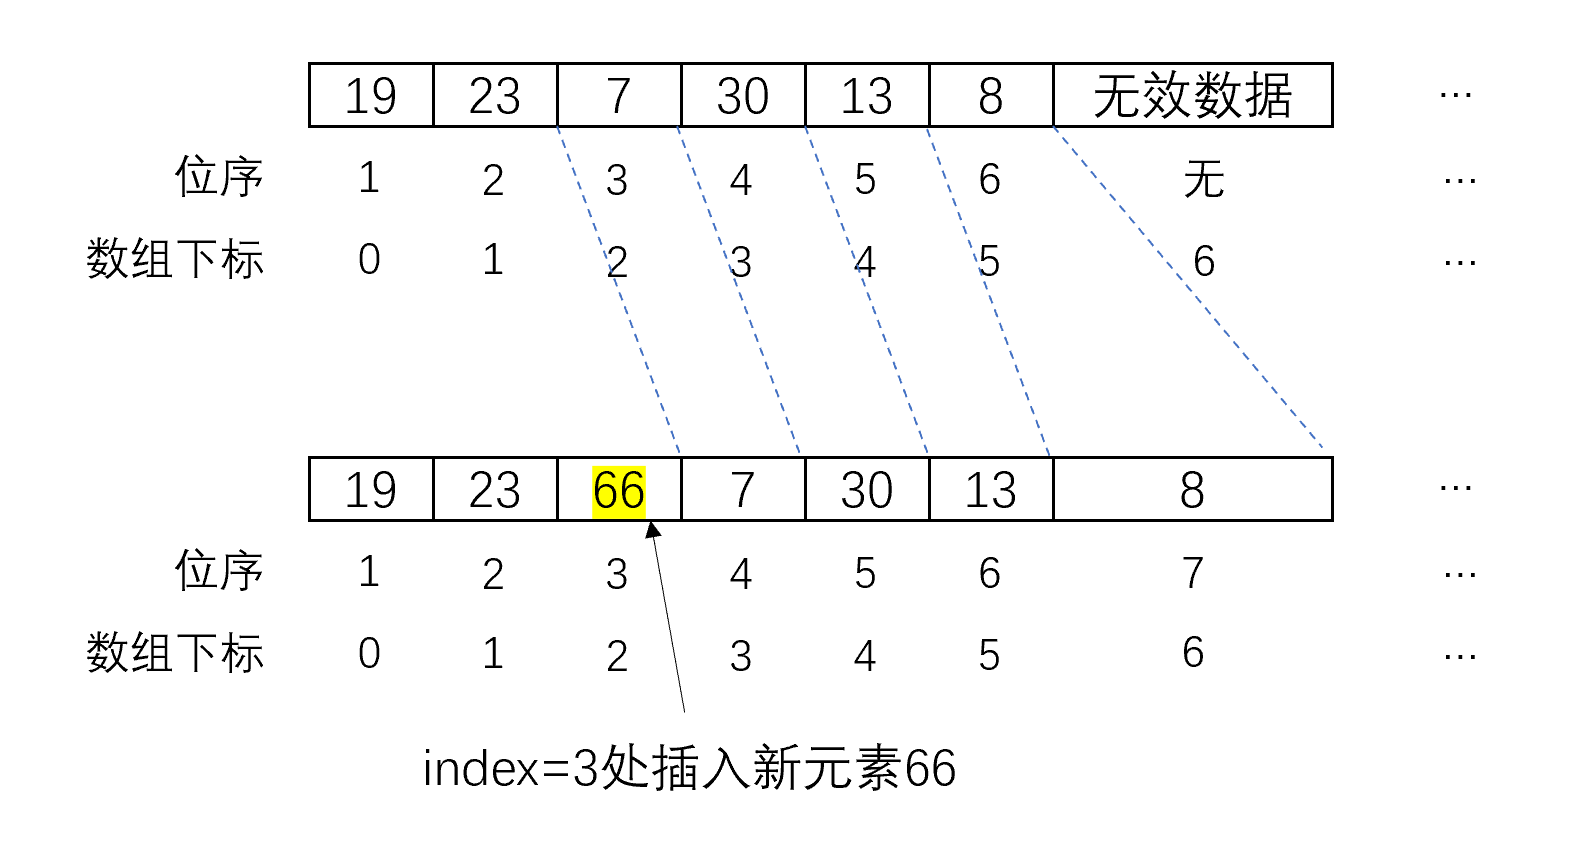
\includegraphics[width=0.55\textwidth]{assets/pics_and_ppts/ch2/顺序表的插入操作.png}}
    \caption{顺序表的插入操作}
    \label{fig:顺序表的插入操作}
\end{figure}
对于顺序表，要在index位置处插入新元素，就要将大量元素依次向右推移一个位置，为新元素腾出位置。显然该算法的瓶颈在于元素移动。不难得出该算法
最好情况下（在表尾插入，无需移动元素）时间复杂度为\(O(1)\)。最坏情况下（在表头插入）元素需要移动n次，\(T(n)=n\)，时间复杂度为\(O(n)\)。
平均情况下，假设在各个位置插入概率相等，则有
\[
    T(n) = \frac{1}{n+1}\cdot 1 + \frac{1}{n+1}\cdot 2 + ... + \frac{1}{n+1}\cdot n = \frac{n}{2}
\]
所以平均情况下，算法时间复杂度为\(O(n)\)。

\minisection{3.顺序表的删除操作}
以下函数实现了操作：将顺序表L中第index个元素删除，并将其值以value变量返回。index=1表示删除表头元素。
\begin{cppcode}
    int DeleteSeqList(struct SeqList *L, int index, ElemType *value) {
    if (index < 1 || index > L->current_size) {
        return -1; // 删除位置非法
    }
    // 将被删元素赋值给变量value
    if (value != NULL) {
        *value = L->data[index-1];
    }
    // 用第index+1个元素（如果有）覆盖第index个元素，并将后面所有元素“前移一格”
    for (int i = index-1; i < L->current_size - 1; i++) {
        L->data[i] = L->data[i + 1];
    }
    L->current_size--;
    return 1;
}
\end{cppcode}
与插入操作的思想类似，显然删除操作的时间复杂度同样为O(n)。
\begin{notebox}{初见提示}
    事实上绝大多数时候我们关注的都是平均复杂度，因此，在未指出“最好”“最坏”或“平均”时，我们提到的“时间复杂度”或“空间复杂度”都是指平均。
\end{notebox}
\begin{insightbox}
    相信这里已经是一个非常合适的位置来指出这几件事：
    \\
    
1.顺序表插入操作的实现代码中，我们规定表满时返回0，插入位置非法时返回-1，插入成功时返回0。为什么要这么规定？为何元素的位序index从1开始算，而不是从0？为何插入操作
名字叫做InsertSeqList？叫别的名字可以吗？
    
    回答：事实上，这些并非死规定，而是由该函数的\uline{实现者}来定义的。如果你来实现这个函数，你当然可以做出其他合理规定，如：“只要插入失败都返回0，只要插入成功就返回1”，
    再如你将函数名起为“SeqListInsert”，这都是可以的，只要你正确地实现了该函数，并给出清晰的说明让该函数的\uline{使用者}知道这个函数具体怎么用就行。类似的事情后面将不再赘述。
    \\
    
2.对于顺序表的删除操作，你也许会问，“删除操作”不就是删掉元素吗？为何还要将被删元素的值返回？这是因为在实际需求中，我们删除一个元素往往需要同时拿到它的值。
    比如，若银心出队去营地休息，我们将她从玩家队伍中移出，可能同时需要将她放入营地，这就需要获取“银心”这一数据元素，因此删除的同时要返回该数据。你当然可以将
    删除操作实现为“只删除，不返回被删元素”，只要你实现得正确。但正如1.1节末尾所指出，本书中每一种数据结构，我们给出的都是较常见的、一般的实现方式。这一点后面将不再赘述。
    \\

    说到这里是时候指出《数据结构》的一个重要思想，请看下面的“3”。
    \\

3.你在解决实际问题时（很可能是某个OJ网站上的问题），在你玩转某个数组的时候，你顺着自己的思路写出的很可能其实就是顺序表的插入、删除等操作，而你决不会把它封装
    成一个函数类似InsertSeqList(...)。但是，《数据结构》的研究在于抽象和封装。
    实际的工程中，你也可以将某个结构及其对应的操作封装好，并和别人说：“这个结构是一棵平衡二叉树，它支持操作123456等、作用分别是xxxxxx，你可以直接拿去用
    （而无需关注其底层是怎么实现的，因为我已经帮你实现好了）”。当然，你最好给出每个接口实现（函数实现）的详细说明，如时间、空间复杂度，各个返回值表示的含义等等。
    相信随着对《数据结构》的研究，你将逐步加深对该思想的体会。
    
\end{insightbox}

\minisection{4.按位序访问/修改元素}
如前所述，顺序表的存储特性决定了它支持随机访问，我们可以直接根据数组下标来访问元素。
\begin{cppcode}
    // 获取位序为index的元素
    int GetElem(struct SeqList *L, int index, ElemType *value) {
        if (index < 1 || index > L->current_size) {
            return -1; // 访问失败
        }
        *value = L->data[index-1];
        return 1;     // 访问成功
    }
    // 将位序为index的元素修改为new_value, 旧值通过value返回
    int SetElem(struct SeqList *L, int index, ElemType new_value, ElemType *value) {
        // 此处略去合法性检查

        *value = L->data[index-1];
        L->data[index-1] = new_value;
        return 1;     // 访问成功
    }
\end{cppcode}
显然该操作时间复杂度为O(1)。
\minisection{5.按值查找元素}
以下函数实现了操作：返回表L中第一个值等于value的元素所在位序。若不存在，返回-1.
\begin{cppcode}
    int SeqListFind(struct SeqList *L, ElemType value) {
        for (int i = 0; i < L->current_size; i++) {
            if (L->data[i] == value) {
                return i+1;
            }
        }
        return -1;
    }
\end{cppcode}
显然该操作时间复杂度为O(n)。{\color{red}\textbf{在后面我们将会看到}}，若顺序表中元素按从小到大或从大到小有序，我们还可以使用\uwave{二分查找}提高查找效率。

到这里我们给出了顺序表的五种常见操作。当然你还可以为它定义更多的操作，如“获取表长”、“判断表是否为空”等操作，感兴趣的同学可以自己尝试实现。
\subsection{从使用者视角理解“数据结构”}
以上我们以“实现者”的视角提供了顺序表这一数据结构及其操作的实现。有了以上实现，我们就有了一个具有基本功能的顺序表可以使用。接下来我们进入“使用者”的视角，
来看一看我们可能会如何使用一个顺序表。我们依然以游戏设计为例。假设你设计的游戏玩法是玩家操控一个四人小队，“出征队伍”最多四人，而你可以随时让“出征队伍”
中的队友去营地休息，也可以随时让营地中的队友加入“出征队伍”。

在你编写代码时，程序启动之初你可能会创建一个用来保存“出征队伍”的顺序表，以及一个用来保存“营地队员”的顺序表并初始化：
\begin{cppcode}
    #define MaxSize 4
    struct RoleSeqList {
        struct Role roles[MaxSize];
        int current_size;
    }
    RoleSeqList expedition_team; // 出征队伍列表
    RoleSeqList camp;    // 营地中的队员列表
    InitList(expedition_team);
    InitList(camp);
\end{cppcode}
游戏之初出征队伍可能只有主角“邪念”一个人，最初你将邪念加入表中：
\begin{cppcode}
    // 假设玩家通过“捏脸”后的数据，或游戏默认的主角初始数据保存在某Role类型的对象"XieNian"中。
    InsertSeqList(expedition_team, 1, XieNian);
\end{cppcode}
而营地中暂时没有队友。随着游戏进行，由于你的好人缘，可能不断有队友“归顺于你”：
\begin{cppcode}
    int result = InsertSeqList(expedition_team, expedition_team.current_size+1, YinXin);    // YinXin入队
    if(result == 0) {
        // 可以在此提示玩家：你的小队最多只能有四个人
    } else if(result == -1) {
        // 错误处理，据实际情况而定
    }
    result = InsertSeqList(expedition_team, ...);   // 其他人入队
    // ...
\end{cppcode}
当你的出征队伍种有了一定数量的人员之后，假设某时刻玩家可能选择让位序为index的人出队并且去营地休息：
\begin{cppcode}
    int result = DeleteSeqList(expedition_team, index, value);  // 位序为index的人出队
    if(result != 1) {
        // ...
    }
    int result = InsertSeqList(camp, camp.current_size, value); // 把这个人放入营地
    if(...) {
        ...
    }
\end{cppcode}
以上便是我们对“顺序表”这一数据结构可能的使用。事实上，游戏中的“出征队伍”和“营地”只是我们为了实现游戏玩法而定义的两个概念。对于顺序表的实现代码来说，
它们并没有什么特殊之处：出征队伍是一个顺序表，营地也是一个顺序表。顺序表并不知道自己保存的Role是何含义，也不知道这些“Role”为什么需要在两个列表之间移动。
它只负责提供一组通用的操作，例如插入、删除、查找和访问。

这正是数据结构的价值所在：我们是在设计一种种通用的数据组织方式，然后在不同的实际问题中重复使用它。

在这个例子中，我们甚至可以进一步把游戏中的具体概念暂时抛开。无论顺序表中存储的是游戏角色、商品，还是其他任何类型的数据，对于顺序表本身而言，它们都只是一个个数据元素。
只要这些元素满足顺序表的基本要求，我们就可以使用同一套数据结构及其操作来管理它们。
因此，从使用者的角度来看，数据结构实际上是一种可以被反复复用的通用工具。它将“如何组织数据”以及“如何操作这些数据”封装起来，使上层程序可以直接利用这些能力
（如直接调用InsertSeqList(camp, camp.current\_size, value)），而不必重复考虑底层的实现细节。这也体现了计算机这门学科一个很重要的思想：“封装”。

至此，相信你已经对《数据结构》这门学科“到底在研究啥”已经有了一个很深刻的认知。此后，除非必要，我们将不再强调类似内容，而专注于《数据结构》本身的研究上。
\section{链表}
在2.1节中我们已经给出了链表存储结构的定义：
\begin{cppcode}
    struct ListNode{
        ElemType data;  // 该节点的数据元素
        struct ListNode* next_node; // 下一个节点的地址 
    };
    typedef struct ListNode* LinkList;
\end{cppcode}
链表的节点通常是通过malloc或new动态分配的，因此逻辑上相邻的节点物理存储上未必相邻。如前所述，我们有了上述定义，就可以像定义一个int变量一样定义一个链表对象my\_linklist。
我们首先给出链表的初始化操作，对于一个定义了但尚未初始化的链表my\_linklist：
\begin{cppcode}
    LinkList my_linklist;  // 此时my_linklist指向未知数据。再次提醒：这个my_linklist语义上既可以表示“一个链表”，也可以表示“该链表的第一个节点指针”
\end{cppcode}
\minisection{1.链表的初始化操作}
初始化一个空的链表，只需要将指向第一个节点的指针置为NULL即可：
\begin{cppcodeNum}[label={code:不带头节点的链表初始化}, codetitle={不带头节点的链表初始化}]
    int InitLinkList(LinkList* L) {
        *L = NULL;
        return 1;
    }
\end{cppcodeNum}
调用
\begin{cppcode}
    InitLinkList(&my_linklist);
\end{cppcode}
即可对my\_linklist这个链表进行初始化。如图\ref{fig:链表初始化前后示意} a）所示。函数将链表第一个节点的指针my\_linklist置为NULL，表示此时表中没有数据元素。
\begin{figure}[htbp]
    \centering
    \fbox{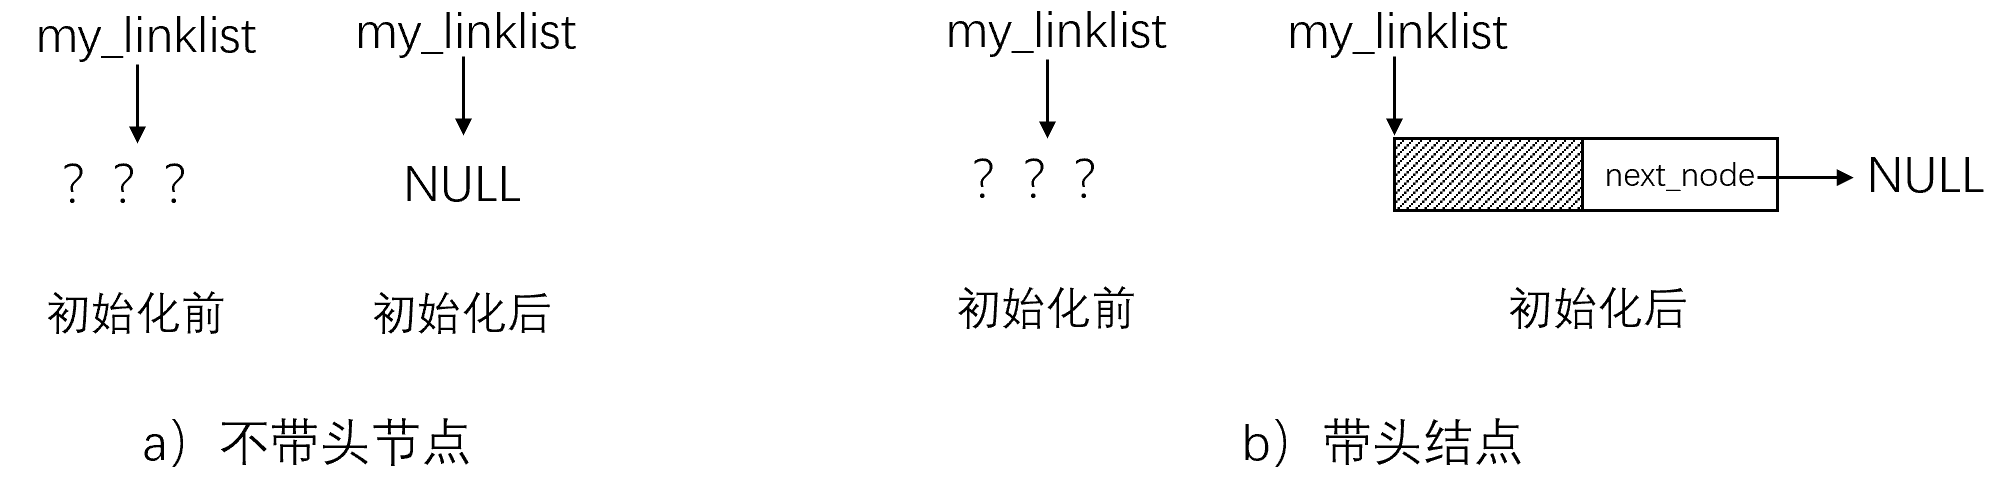
\includegraphics[width=0.78\textwidth]{assets/pics_and_ppts/ch2/链表初始化前后示意.png}}
    \caption{链表初始化前后示意}
    \label{fig:链表初始化前后示意}
\end{figure}
事实上，为了操作上的方便，我们在实现链表时，通常在表的第一个\uline{有效的数据节点}之前附加一个节点，称为\term{头节点}，如图\ref{fig:带头节点与不带头节点的链表}所示。
头节点同样可以用ListNode结构来定义，只不过这个节点不保存有效数据（data字段可以不填值），而仅仅是链表的实现者为了代码简单易实现、不出错而额外引入的一个辅助节点。
\begin{figure}[htbp]
    \centering
    \fbox{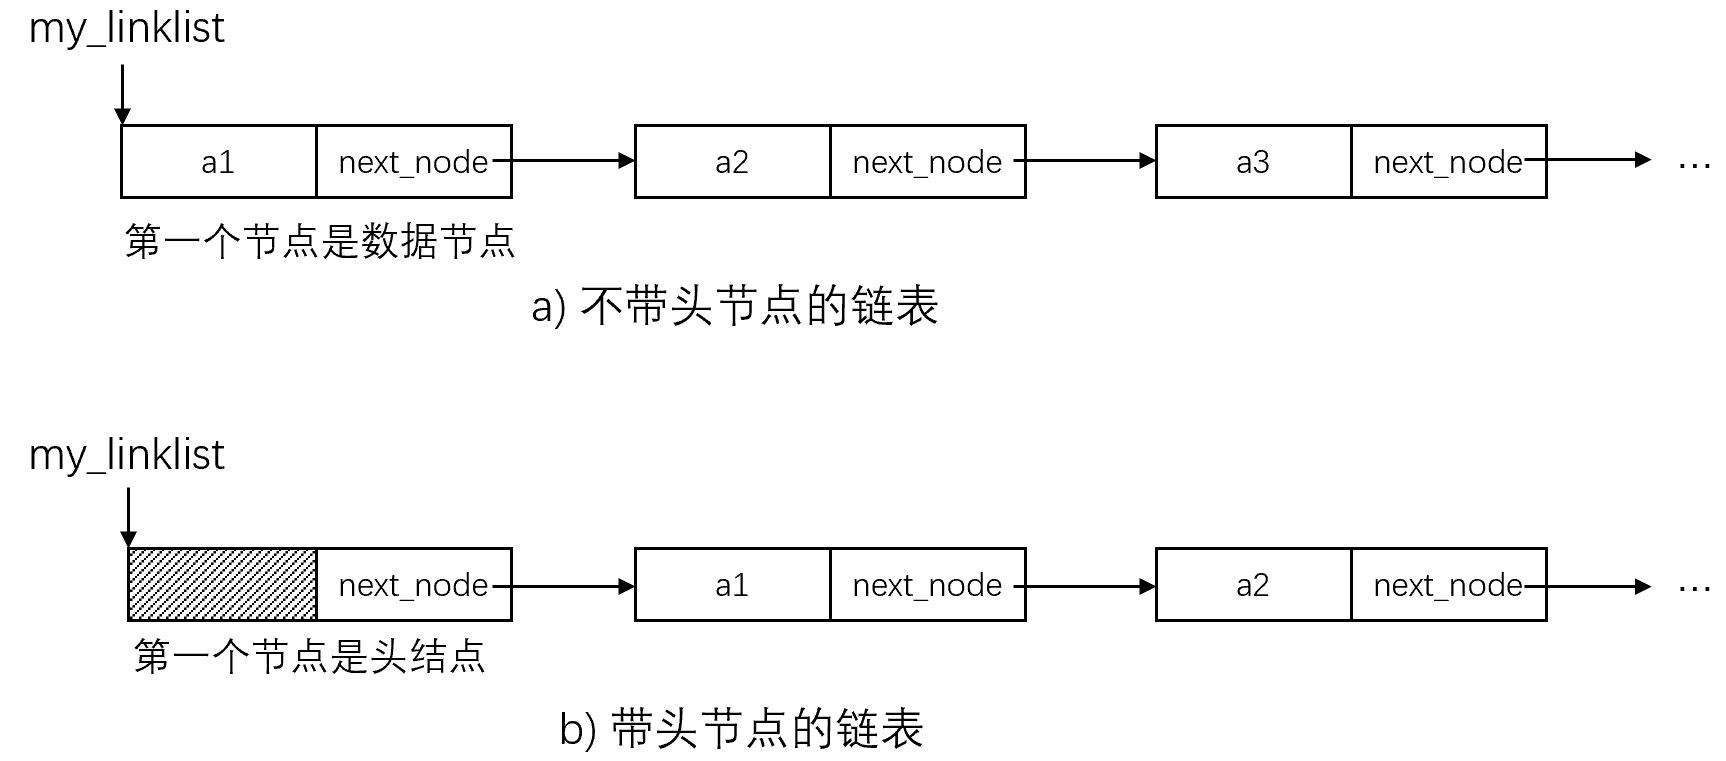
\includegraphics[width=0.9\textwidth]{assets/pics_and_ppts/ch2/带头节点与不带头节点的链表.png}}
    \caption{带头节点与不带头节点的链表}
    \label{fig:带头节点与不带头节点的链表}
\end{figure}

\begin{notebox}{提示}
    （特别是北方的朋友）请注意，对于带\term{头节点}的链表，头节点确实等同于“头一个节点”，即第一个节点。而对于不带\term{头节点}的链表，不能把第一个节点叫做“头节点”，
    “头节点”是一个专有名词，而不是表达“头一个节点”的语义。
\end{notebox}

引入了头节点后，头节点即第一个节点，因此对于带头节点的链表，第一个节点的指针就是指向头节点的指针。带头节点的链表初始化操作代码如下：
\begin{cppcodeNum}[label={code:带头节点的链表初始化}, codetitle={带头节点的链表初始化}]
    int InitLinkList(LinkList* L) {
        *L = (ListNode*)malloc(sizeof(ListNode));    // 创建头节点
        if(*L == NULL) {
            return 0;
        }
        (*L)->next_node = NULL;    
        return 1;
    }
\end{cppcodeNum}
初始化过程如图\ref{fig:链表初始化前后示意} b）所示。

\begin{notebox}{提示}
    在代码\ref{code:不带头节点的链表初始化}及代码\ref{code:带头节点的链表初始化}中，LinkList本身类型是ListNode*，因此LinkList* 的类型是ListNode**,
    是一个二级指针。所以*L类型是ListNode*，即指向某链表节点的指针。
    
    要在函数栈内改变栈外普通变量的值就要用其指针作为参数传递。而栈外的变量my\_linklist本身是一个指针，因此要在函数栈内改变其值，就要用指针的指针。

    如果你熟悉C++，就可以使用C++中的引用传参来解决多级指针带来的理解上的问题。后续内容中在一些地方我们将使用引用降低语言本身带来的理解负担，这样可以将更多精力专注于
    《数据结构》本身的思想。
\end{notebox}
由于带头结点的链表更常用，如无特殊说明，本节中均默认链表带头结点。

\minisection{2.销毁链表}
销毁链表与初始化相对应。销毁链表需要释放每个节点的内存空间。
\begin{cppcode}
    void DestroyLinkList(LinkList* L) {
        struct ListNode* p = *L;    // p始终指向当前待释放位置
        struct ListNode* q;
        while (p != NULL) {
            q = p->next_node;       // q是下一个待释放位置
            free(p);
            p = q;
        }
        *L = NULL;
    }
\end{cppcode}
这里需要注意，第7行不能写成“p = p->next\_node”。因为p在第6行已经被释放了，再访问p会导致未定义行为。这也是为什么要先用q保存p的值。
\minisection{3.判断链表是否为空}
由于我们采用的是带头结点的设计，因此第一个节点的next\_node指针指向的才是实际的第一个数据元素节点。
\begin{cppcode}
    int ListIsEmpty(LinkList L) {
        return L->next_node == NULL;
    }
\end{cppcode}

\minisection{4.求链表长度}
求链表长度的操作是计算链表中数据节点的个数。对于链表，我们想要求得表长就需要遍历一遍链表，每访问到一个有效的数据节点就将计数器加一，最后得到表长。
\begin{cppcode}
    int GetLength(LinkList L) {
        int length = 0;
        struct ListNode* p = L->next_node;  
        while (p != NULL) {
            length++;
            p = p->next_node;
        }
        return length;
    }
\end{cppcode}
显然求链表长度操作的时间复杂度为O(n)。另外请注意，链表长度是不包括头结点的，这一点很好理解。

\begin{insightbox}
    事实上，我们可以对LinkList类型做进一步的封装，类似：
    \begin{cppcode}
        struct WrappedLinkList {
            LinkList L;
            int elem_num;   // 额外增加的变量
        };
    \end{cppcode}
    通过额外维护一个变量elem\_num实时记录当前链表的元素数量，链表初始化时该变量赋值0，插入时加一，删除时减一。这样可以做到O(1)时间求链表的长度。熟悉C++的同学
    可以知道，C++标准库中的std::list就是采用了类似的实现方式，所以std::list的size()方法时间复杂度为O(1)。
\end{insightbox}

\minisection{5.在第i个位置插入元素}
在链表L中的第i个位置插入一个值为e的新节点s，需要断开原来的链条，将新元素“链接上”，其过程如图\ref{fig:链表的插入过程示意}所示。
\begin{figure}[htbp]
    \centering
    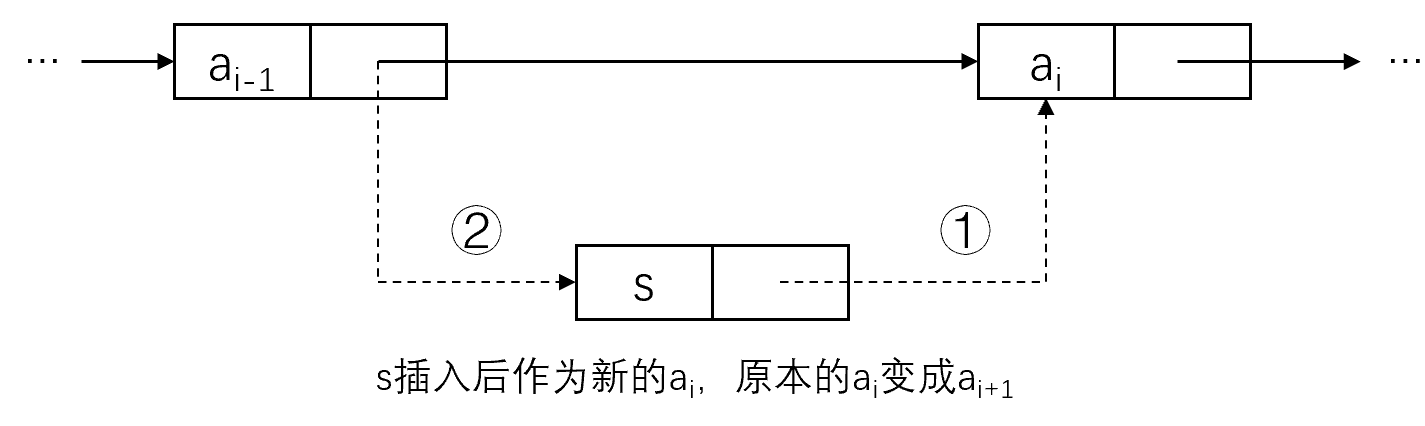
\includegraphics[width=0.7\textwidth]{assets/pics_and_ppts/ch2/链表的插入过程示意.png}
    \caption{链表的插入过程示意}
    \label{fig:链表的插入过程示意}
\end{figure}
实现代码如下。
\begin{cppcode}
    int ListInsert(LinkList L, int i, ElemType e) {
        struct ListNode* p = L;
        // 找到第 i-1 个节点
        for (int j = 1; j < i; j++) {
            if (p->next_node == NULL)
                return 0;   // 插入位置有误
            p = p->next_node;
        } // 该循环结束后，p指向第i-1个节点@\(a_{i-1}\)@
        // 创建新节点
        struct ListNode* s = (struct ListNode*)malloc(sizeof(struct ListNode));
        s->data = e;
        // 插入节点
        s->next_node = p->next_node;    // @\Circled{1}@
        p->next_node = s;               // @\Circled{2}@
        return 1;
    }
\end{cppcode}
可以看到在第i个及第i-1个节点之间插入，要操作链条，就要拿到这两个节点的信息。这也是该算法的主要开销：找到这两个节点的指针。
不难看出该算法时间复杂度为O(n)。通过该例大家也能出头结点所带来的好处之一——简化边界处理：即使插入位置是表首，也不需要特殊处理。
\begin{notebox}{初见提示}
    相信你发现了，代码第十行我们分配内存后没检测是否分配成功。在之后的诸多场景，我们将略去类似代码，而专注于算法的核心思想上。
\end{notebox}

\minisection{6.删除第i个元素}
同插入操作的思想类似，删除操作的核心同样是链条操作，如图\ref{fig:链表的删除过程示意}。
\begin{cppcode}
    int ListDelete(LinkList L, int i, ElemType* e) {
    struct ListNode* p = L;
    struct ListNode* q;
    // 找到第 i-1 个节点
    for (int j = 1; j < i; j++) {
        if (p->next_node == NULL)
            return 0;
        p = p->next_node;
    }
    if (p->next_node == NULL)
        return 0;
    q = p->next_node;
    if (e != NULL)
        *e = q->data;
    // 删除节点
    p->next_node = q->next_node;
    free(q);
    return 1;
}
\end{cppcode}
显然该算法时间复杂度同样为O(n)。
\begin{figure}[htbp]
    \centering
    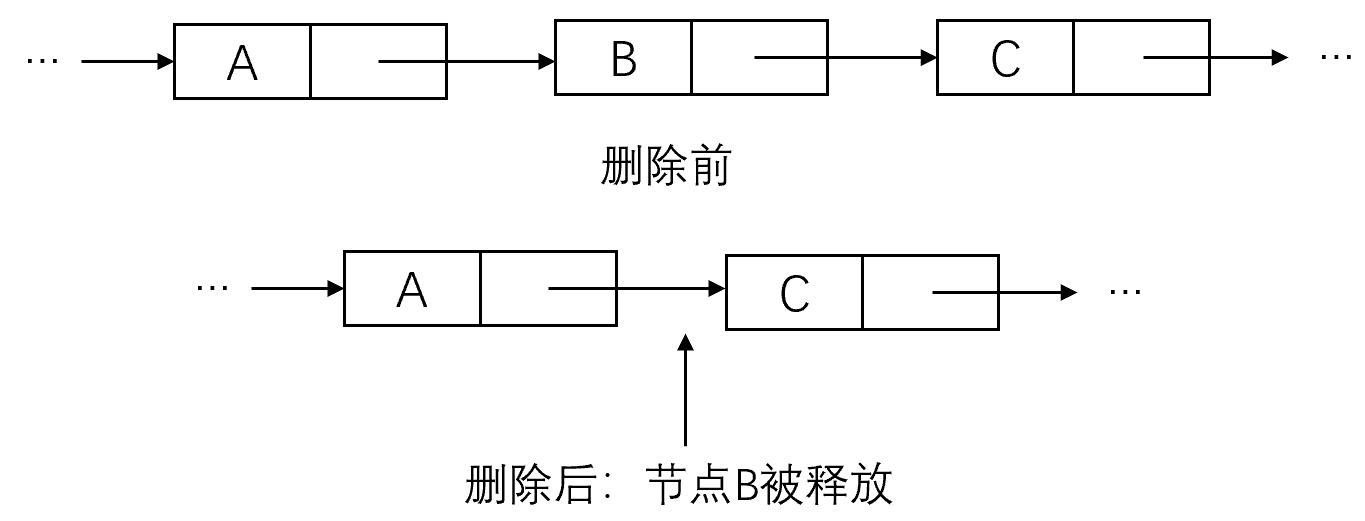
\includegraphics[width=0.7\textwidth]{assets/pics_and_ppts/ch2/链表的删除过程示意.png}
    \caption{链表的删除过程示意}
    \label{fig:链表的删除过程示意}
\end{figure}

\minisection{7.按位置获取元素}
由于链表的存储结构，其无法直接通过访问位置i计算得到元素的地址，而只能从第一个节点顺着链条一个一个往下找。代码实现如下：
\begin{cppcode}
    int GetElem(LinkList L, int i, ElemType* e) {
        struct ListNode* p = L->next_node;
        // 控制指针p始终指向第j个数据节点，j==i成立时，循环结束，p指向第i个节点，即要找的节点
        for (int j = 1; j < i; j++) {
            if (p == NULL)
                return 0;
            p = p->next_node;
        }
        if (p == NULL)
            return 0;
        *e = p->data;
        return 1;
    }
\end{cppcode}
前面我们说链表只能顺序访问（sequential access），而不能随机访问（random access），这里我们也从代码的角度进一步认识了这一点。并且同时我们
不难看出，要修改位序为i的节点，思想和该GetElem函数非常相似，只不过把获取元素变成了修改元素。

至此，我们已经对链表进行了较为深入的探讨。请大家注意，以上我们所谈的“链表”也可以叫做\term{“单链表”}，因为它只有由前指向后的一条“单链”，而没有由后指向前的链条。
事实上，链表还有多种变态，用于灵活地适应不同需求，我们将在{\color{red}\textbf{接下来的章节中展开讨论}}。




\section{顺序表与单链表的对比}
顺序表和单链表都是线性表的常见实现方式，它们都能够表示一组具有线性关系的数据。二者最大的区别在于数据的存储方式不同：
\begin{itemize}
    \item 顺序表使用一段连续的存储空间保存数据，元素之间通过下标表示逻辑关系；
    \item 链表通过指针将多个离散存储的结点连接起来，元素之间通过指针表示逻辑关系。
\end{itemize}
这种存储方式的不同，决定了二者具有不同的特点。
\subsection{随机访问}
由于顺序表中的元素连续存储，因此可以通过下标直接计算元素地址，访问任意位置的元素只需要 $O(1)$ 时间。
因此，顺序表适合需要频繁随机访问的场景。

而单链表中的结点在内存中通常不是连续存储的，无法根据位置直接计算地址。如果想访问第 $i$ 个元素，必须从第一个结点开始依次遍历，因此时间复杂度为 $O(n)$。
\subsection{插入和删除}
\label{subsec:插入和删除}
顺序表在插入或删除元素时，通常需要移动若干元素。因此，顺序表的插入和删除操作平均时间复杂度为 $O(n)$ 。


而链表中的结点通过指针连接。
插入元素只需要修改相关结点的指针关系，就可以完成插入或删除操作，不需要移动其他元素。在已经拿到节点指针的情况下，单链表的插入操作时间复杂度为 $O(1)$，但删除操作
的时间复杂度仍然为O(n)。
即使没提供节点指针，而只提供了插入位序i：ListInsert(LinkList L, int i, ElemType e); 此时虽然插入的时间复杂度为O(n)，但是该算法的主要开销在于找到插入位置，主要
操作是“比较”，而非“移动”，因此虽然都是O(n)，但链表的插入或删除操作也比线性表更快。


\subsection{空间利用}
顺序表需要一段连续的存储空间，并且通常需要提前申请一定容量。如果申请空间过大，会造成浪费；如果空间不足，则可能导致一些后果。

而链表不要求连续存储空间，可以根据需要动态创建结点，因此空间利用更加灵活。但是，链表中的每个结点需要额外保存指针信息，因此会增加额外的存储开销。


\subsection{如何选择}
顺序表和链表没有绝对的优劣，它们分别适用于不同的问题场景。二者总结如下表：

\begin{center}
\begin{tabular}{c|c|c}
 & 顺序表 & 链表 \\
\hline
存储方式 & 连续存储 & 离散存储 \\
随机访问 & $O(1)$ & $O(n)$ \\
插入删除 & $O(n)$ & $O(1)$或$O(n)$，但更快\\
空间利用 & 不灵活 & 动态申请,较灵活 \\
额外空间开销 & 较小 & 需要保存指针,较大 \\
\end{tabular}
\end{center}

因此：

\begin{quote}
如果程序需要频繁访问任意位置的数据，顺序表通常更加合适；

如果程序需要频繁进行插入和删除操作，链表通常更加合适。

...
\end{quote}

通过本节内容也给了我们一个启示：数据结构的设计，甚至很多工程上的设计，都是在不同需求之间进行权衡，一种设计提高了某方面的表现，通常也会付出其他方面的代价。
我们要在不同需求场景下灵活地进行取舍。

\begin{insightbox}
    请你思考这样一个问题：遍历线性表，如以下伪代码：
    \begin{cppcode}
        void TravelList(List L) {
            for( every data in L ) {
                do_something();
            }
        }
    \end{cppcode}
    顺序表和链表哪个更快？\\
    
    我们先来看二者的遍历代码。顺序表的遍历：
    \begin{cppcode}
        for (int i = 0; i < n; i++) {
            visit(arr[i]);
        }
    \end{cppcode}
    每次访问arr[i]前，要计算其地址：arr[i]=arr[0]+(i-1)*sizeof(ElemType). 之后访问内存；链表的遍历：
    \begin{cppcode}
        Node* p = head;
        while (p != NULL) {
            visit(p->data);
            p = p->next;
        }
    \end{cppcode}
    可以看到，链表的遍历是没有乘法操作的。从硬件角度讲，乘法操作是一种很慢的操作。那是不是链表的遍历就比顺序表快呢？并不是。

    我们还要考虑一点：现代计算机有一个非常重要的机制：\term{Cache（高速缓存）}。大家如果了解过《计算机组成原理》或《操作系统》相关内容应该已经恍然大悟了。

    什么是Cache（高速缓存）？这其实也是这门学科一个非常重要的思想，操作系统的实现、高并发服务的架构设计等许多场景下都有Cache的思想。它基于一个经验性
    规律，叫做\term{程序的局部性原理}：

    程序在运行过程中，访问的数据和指令往往不是随机分布的，而是在一段时间内集中访问某些局部区域。具体来说：
    \begin{itemize}
        \item 如果一个数据或指令最近被访问过，那么它近期很可能再次被访问。
        \item 如果一个数据被访问，那么它附近的数据近期也很可能被访问。
    \end{itemize}
    Cache的设计思想就是，将部分“近期可能频繁被访问的数据”装入更高速的设备中，来提升程序的运行性能。举个例子，某大型3D游戏的地图非常大，有10个GB，
    程序并非会将所有地图数据都装入主存，而是只装载玩家所在位置附近的地图，玩家移动到新区域或进行传送等操作，再进行主存和磁
    盘的“数据交换”，将新区域的地图装入主存。在这个场景下，我们可以称“主存”是“磁盘”的“Cache（高速缓存）”。\\

    事实上，现代计算机都会有比内存更高速的缓存，通常称作CPU Cache。根据局部性原理，将近期常用的指令和数据从主存装入CPU Cache，来提升程序的运行性能。
    说到这里，大家应该发现了，对于顺序表，由于其物理连续的存储特性，它的“局部性”是更好的。同一个顺序表极有可能同时被装入CPU Cache。而链表则不同，遍历链表
    时，会发生频繁的CPU Cache和主存的“数据交换”，这种“抖动”会带来极大的性能损耗。\\

        顺序表虽然存在乘法操作，但其局部性更好，而且，现代编译器通常会做出非常棒的编译优化，对于顺序表的遍历代码，可以将乘法操作带来的影响降得很低很低。所以，
    对于遍历操作，顺序表和链表哪个更好，这个问题没有统一的结论，但通常我们认为，在数据量较大时，顺序表的遍历是更快的。
\end{insightbox}


\clearpage%%%%%%%%%%%%%%%%%%%%%%%%%%%%%%%%%%%%%%%%%%%%%%%%%%%%%%%%%%%%%%%%%%%%%%%%%%%%%%%%%%%%%%%%%%%%%%%%%%%%%%%%%%%%%%%%%%%%%%%%%%%%%%
\begin{exercise}
1. 关于线性表，下列说法正确的是（　）。\\
A. (银心, 甘尔, 张三) 和 (甘尔, 银心, 张三)是两个相同的线性表 \\
B. 线性表是一种物理结构，线性表的所有元素物理地址一定连续\\
C. 同一个线性表中各个元素的数据类型可以不同\\
D. 不同线性表的数据元素类型可以不同\\

2. 对于顺序表，假设表中已有 \(n\) 个元素，下列操作中时间复杂度一定为 \(O(1)\) 的是（　）。\\
A. 在表中某位置插入一个元素\\
B. 删除表头元素\\
C. 获取第 \(i\) 个位置上的元素\\
D. 查找值为 \(x\) 的元素\\

3. 对于一个带头结点的单链表：
\begin{bulk}
head → A → B → C → NULL
\end{bulk}
若 p 指向节点 A，现在希望在 A 后面插入节点 X，正确的核心操作是（　）。\\
A. p->next\_node = X;
X->next\_node = p->next\_node;\\
B. X->next\_node = p;
p->next\_node = X;\\
C. X->next\_node = p->next\_node;
p->next\_node = X;\\
D. p = X;
X->next\_node = p->next\_node;\\

4. 以下单链表的操作中，时间复杂度一定是O(1)的是（  ）。\\
A. 求表长\\
B. 在表头插入元素\\
C. 在表尾插入元素\\
D. 获取第\(i\)个位置上的元素\\

5. 在\coderef{code:线性表的顺序存储结构}中，我们存储顺序表元素使用的数组是静态存储的，定义其最大存储数量为100.若存满了，则无法再扩充。事实上，
我们可以使用malloc动态分配数据元素的存储空间，而只保存一个该空间的起始地址指针：
\begin{cppcode}
    struct SeqList{  
        ElemType* data;         // 数组起始地址
        int current_size;       // 当前表中的元素数量
        // ...
    };
\end{cppcode}
请你想一想，动态存储下，会有哪些操作和静态存储不同？（重点思考一下插入操作）\\

6. 假设数组a中下标0-9处存放了10个int型数据\(a_1\)-\(a_{10}\)，请你用数组a中的数据分别构建以下两个链表，填充对应代码：

1） \(a_1\) → \(a_2\) → ... → \(a_{10}\)
\begin{cppcode}
    LinkList f1(int a[], int n=10) {

    }
\end{cppcode}
2） \(a_{10}\) → \(a_9\) → ... → \(a_1\)
\begin{cppcode}
    LinkList f2(int a[], int n=10) {

    }
\end{cppcode}
建议采用带头结点的实现。\\

7. 请你实现一个算法DeleteValue(LinkList L, ElemType e)，删除带头结点的单链表L中所有值等于e的节点。\\




% 8. 【某年408真题】已知一个带头节点的单链表，节点结构为
% \begin{cppcode}
%     struct ListNode {
%         ElemType data;
%         ListNode* link;
%     };
% \end{cppcode}
% 假设该链表只给出了头指针list。在不改变链表的前提下，请设计一个尽可能高效的算法，查找链表中倒数第k个位置上的节点（k为正整数）。若查找成功，算法输出
% 该节点的data域的值，并返回1；否则，只返回0.要求：\\
% 1）描述算法的基本设计思想；\\
% 2）描述算法的详细实现步骤；\\
% 3）根据设计思想和实现步骤，采用C、C++或Java语言实现算法，关键之处给出简要注释。\\

8. 假设线性表采用带头结点的单链表保存，结点定义如下：
\begin{cppcode}
    typedef struct node
    {
        int data;
        struct node *next;
    }NODE;
\end{cppcode}
请你设计一个尽可能高效的算法，对于任意输入的链表L，都能返回其中间节点。
当表长为奇数时，返回中间的那个节点；当表长为偶数时，返回中间两个节点中左边（位序更小）的那个；当表为空表时，返回空指针NULL。\\

9. 

1）请你设计实现将带头结点的单链表逆置的算法。即：将
\begin{bulk}
    \begin{center}
        head → \(a_1\) → \(a_2\) → ... → \(a_n\)
    \end{center}
\end{bulk}
变为
\begin{bulk}
    \begin{center}
        head → \(a_n\) → \(a_{n-1}\) → ... → \(a_1\)
    \end{center}
\end{bulk}

2）设计实现将不带头结点的单链表逆置的算法。\\


10. 【某年408真题】设线性表：
$$ L=(a_1,a_2,a_3,\cdots,a_{n-2},a_{n-1},a_n) $$
采用带头结点的单链表保存，链表中的结点定义如下：
\begin{cppcode}
    typedef struct node
    {
        int data;
        struct node *next;
    }NODE;
\end{cppcode}

请设计一个空间复杂度为 \(O(1)\) 且时间上尽可能高效的算法，重新排列 \(L\) 中的各结点，得到：
$$ L'=(a_1,a_n,a_2,a_{n-1},a_3,a_{n-2},\cdots) $$
要求：\\
1）给出算法的基本设计思想；\\
2）根据设计思想，采用 C 或 C++ 语言描述算法，关键之处给出注释；\\
3）说明所设计算法的时间复杂度。\\
\end{exercise}
\clearpage


% 给出习题答案。exerciseanser部分的内容会被main.tex中的\printanswers收集并打印。
\begin{exerciseanswer} 
1. D。线性表要求元素存在位置上的逻辑关系，A错误；线性表是一种逻辑结构，通常可以用数组或链表实现，B错误；线性表要求同一个表中的数据类型相同，C错误；实际需求中我们
要处理int型的数据，就会使用一个int型的线性表，要处理Role类型的数据，就会使用Role类型的线性表，D正确。\\

2. C。A、B选项都需要移动若干元素，时间复杂度为O(n)；D项需要从表头开始，将每一个元素的值与x对比直至找到，时间复杂度为O(n)。C项，由于每个元素
的地址可以由其位序直接计算得来，因此时间复杂度为O(1)。\\

3. C。\\

4. B。由于链表结构中保存有表首元素指针，因此在表头插入元素时间复杂度一定是O(1)。对于C选项，要在单链表的表尾插入元素，需要先遍历链表，拿到尾节点的指针，再
操作链条，时间复杂度为O(n)。我们将在后面看到，为了解决单链表无法高效在尾部插入元素的问题，可以通过单链表的多种变态解决，如：记录尾指针的
\uwave{循环单链表}、\uwave{循环双链表}等。\\

5. 事实上，这种存储方式下，还需要一个字段capacity标记当前已动态分配的空间总量：
\begin{cppcode}
    struct SeqList {
        ElemType* data;     // 数组起始地址
        int current_size;  // 当前表中的元素数量
        int capacity;      // 当前已分配的数组容量
    };
\end{cppcode}
例如：capacity = 100，current\_size = 80表示分配了100个位置的内存空间，目前使用了80个，还剩20个。操作方面，显然，初始化动态分配版本的顺序表需要
为data分配一个初始空间，初始分配多大你可以自己定义。除初始化外，这里我们仅指出一个重点操作：插入。 

回忆静态存储的顺序表，若表满，只能拒绝插入（当然你可以规定淘汰算法，接受新值淘汰旧值，这取决于你，但静态存储已经无法存储更多了）。而动态存储版本，
当已分配空间满了的时候，我们可以申请一块更大的内存空间，将已有表中数据整体拷贝过去，并接受新元素。C++中的std::vector就采用了类似机制实现。\\

6. 拟采用带头节点的实现。代码如下：

1）要构建\(a_1\) → \(a_2\) → ... → \(a_{10}\)，不难想出，只需要按顺序将每一个元素依次链接到链表尾部就可以，代码如下：
\begin{cppcode}
    LinkList f1(int a[], int n = 10) {
        // 创建头结点
        LinkList head = (int*)malloc(sizeof(ListNode));
        head->next_node = NULL;     
        // 动态维护tail，让其始终指向当前链表最后一个节点
        LinkList tail = head;
        for (int i = 0; i < n; i++) {
            LinkList node = (int*)malloc(sizeof(ListNode));   // 为新数据分配一个节点
            node->data = a[i];
            node->next_node = NULL;
            // 新节点插入在最后一个节点之后（尾插）
            tail->next_node = node;
            tail = node;    // 动态维护tail指针，让tail始终指向最后一个节点
        }
        return head;
    }
\end{cppcode}

    2）要构建\(a_{10}\) → \(a_9\) → ... → \(a_1\)，实际也很简单，只需要按顺序将每一个元素依次插入链表头部即可，代码如下：
    \begin{cppcode}
        LinkList f2(int a[], int n = 10) {
            // 创建头结点
            LinkList head = new ListNode;
            head->next_node = NULL;
            for (int i = 0; i < n; i++) {
                LinkList node = new ListNode;
                node->data = a[i];
                // 新节点插入在头结点之后（头插）
                node->next_node = head->next_node;
                head->next_node = node;
            }
            return head;
        }
    \end{cppcode}
    事实上，函数f1就是许多经典教材中\term{“尾插法”}的实现，函数f2就是\term{“头插法”}的实现。\\


7. 思路：遍历一遍链表，“检查”每一个节点的值，若等于e，将其删除，并重构该节点附近链条。代码如下。
\begin{cppcode}
    void DeleteValue(LinkList L, ElemType e) {
        ListNode* pre = L;          // 当前“检查”的节点的前驱节点
        ListNode* cur = L->next_node; // 当前“检查”的节点
        while (cur != NULL) {
            if (cur->data == e) {
                ListNode* temp = cur;
                // 重构链条
                pre->next_node = cur->next_node;
                // 推移cur指针，准备检查下一个节点
                cur = cur->next_node;
                // 释放删除节点
                free(temp);
            }
            else {
                // 当前节点不是目标节点
                // 前驱和当前节点同时后移, 继续检查下一个节点
                pre = cur;
                cur = cur->next_node;
            }
        }
    }
\end{cppcode}

8. 相信大家很自然地就能想到的一种做法是：先遍历一遍链表，计算出表长n，再从头开始查找\(\frac{n+1}{2}\)位置处的节点将其返回。代码如下：
\begin{cppcode}
    NODE* FindMiddle1(NODE *L) {
        int n = 0;
        // 第一次遍历，统计节点数量
        NODE *p = L->next;  // 带头结点，L->next是第一个数据节点
        while(p != NULL) {
            n++;
            p = p->next;
        }
        // 空表情况
        if(n == 0)
            return NULL;
        // 第二次遍历，寻找第(n+1)/2个节点
        int pos = (n + 1) / 2;
        p = L->next;    // p指针重置为第一个数据节点，从这里开始找
        for(int i = 1; i < pos; i++) {
            p = p->next;
        }
        return p;
    }
\end{cppcode}

事实上，还有一种更高效的算法，就是所谓的经典的\term{“双指针算法”}。我们设置两个指针，slow指针每次走一步，fast指针每次走两步，这样，slow“走过的里程”永远是fast的
一半，所以，当fast走到表尾时，slow就处在中间。需要注意的就是边界判断及奇偶的处理。代码如下：
\begin{cppcode}
    NODE* FindMiddle2(NODE *L) {
        NODE *slow = L->next;
        NODE *fast = L->next;
        if(slow == NULL)
            return NULL;
        while(fast->next != NULL && fast->next->next != NULL) {
            slow = slow->next;
            fast = fast->next->next;
        }
        return slow;  
    }
\end{cppcode}

9. 本题思路很简单。对于带头节点的单链表，我们依次将（本来就在头节点后的\(a_1\)、）\(a_2\)、\(a_3\)、...、\(a_n\)插入到第一个数据节点之前（即头节点之后）就行。
我们动态维护指针p，让其指向当前“待插”节点。代码如下。
\begin{cppcode}
    NODE* Reverse(NODE* L) {
        NODE* p = L->next;  // L是头节点，L->next是第一个数据节点
        L->next = NULL;     // 插入过程中，让链表的“已定形部分”的尾节点指向NULL
        while(p) {
            // next为下一个待插节点
            NODE* next = p->next;
            // 插入当前节点
            p->next = L->next;
            L->next = p;
            // 动态维护p，使其指向下一个待插节点
            p = next;
        }
        return L;
    }
\end{cppcode}
这个过程其实也可以理解为按顺序将当前链表节点用头插法{\color{red}\textbf{（见习题1 第6小题）}}“重新插入该链表”。

对于不带头结点的单链表同样是将每一个节点依次插入到第一个数据节点之前：
\begin{cppcode}
    NODE* Reverse(NODE* L) {
        NODE *new_head = NULL;
        NODE *p = L;
        while(p != NULL) {
            NODE *next = p->next;
            p->next = new_head;
            new_head = p;
            p = next;
        }
        return new_head;
    }
\end{cppcode}

10. 经过观察分析不难看出，题目要我们将“倒数第i个元素”插入到“第i个元素”后面，换句话说，如果我们将链表从正中间“砍成两半”，题目要求的正是我们将链表的“后半部分”
从后往前依次插入“前半部分”中。大家可能会想，后半部分如果有反向链条就好了对吧？就可以依次一个一个插入了。那没有，怎么办呢？
相信聪明的你已经想到了，在第上一个习题中，我们介绍了链表的倒置算法。我们将后半部分链表倒置一下不就可以了？没错！接下来我们就给出本题的完整思路：

我们先用双指针算法（见习题1 第8小题）找到链表的中点，将链表砍成两半。然后将后半部分链表逆置，再依次插入前半部分的对应位置中。

若元素个数为奇数个，那“中点”应该分给第一部分还是第二部分呢？其实经过简单的思考不难发现：其实给哪部分都行，我们是可以通过代码控制的。

完整的代码实现如下：
\begin{cppcode}

void Rearrange(NODE *head) {
    if(head == NULL || head->next == NULL)
        return;
  
    // 双指针寻找链表中点，slow最终指向第一部分的最后一个节点
    NODE *slow = head;
    NODE *fast = head;
    while(fast->next != NULL &&
          fast->next->next != NULL) {
        slow = slow->next;
        fast = fast->next->next;
    }
    /* 将链表“砍成两半”
     * 第一部分:
     * head->next ... slow
     * 第二部分:
     * second-> ...
     */
    NODE *second = slow->next;  // second即第二部分的“第一个节点”。注意：第二部分事实上是一个“不带头结点”的单链表，其第一个节点就是second指向的数据节点。
    slow->next = NULL;
    /*
     * 第二步：
     * 逆置第二部分链表
     */
    NODE *prev = NULL;
    NODE *cur = second;
    while(cur != NULL) {
        NODE *next = cur->next;
        cur->next = prev;
        prev = cur;
        cur = next;
    }
    second = prev;
    /*
     * 第三步：
     * 交替合并两个链表
     */
    NODE *first = head->next;
    NODE *p = first;    // 动态维护p，让其始终指向第一部分的插入位置
    NODE *q = second;   // 动态维护q，让其始终指向第二部分的待插节点
    while(p != NULL && q != NULL) {
        NODE *pNext = p->next;
        NODE *qNext = q->next;
        // 插入q节点
        p->next = q;
        q->next = pNext;
        // 推移p和q两个指针，准备插入下一个节点
        p = pNext;
        q = qNext;
    }
}
\end{cppcode}
寻找中点、逆置第二部分链表和交替合并的过程时间复杂度均为O(n)，因此整个算法时间复杂度为O(n)。





\end{exerciseanswer}    %%%%%%%%%%%%%%%%%%%%%%%%%%%%%%%%%%%%%%%%%%%%%%%%%%%%%%%%%%%%%%%%%%%%%%%%%%%%%%%%%%%%%%%%%%%%%%%%%%%%%%%%%%%%%%%%%%%%%%%%%%%%%%



\section{单链表的常见变态}
\subsection{双链表}
单链表的节点只有一个指向其后继的指针，如果我们要访问某个给定节点的前驱，还是要从头开始遍历。很多人会想到，如果我有这样的需求：频繁地访问某个给定节点的前驱
节点{\color{red}\textbf{（例如习题1 第10题）}}，是不是可以在链表的结构定义中增加一个指针prior\_node，指向该节点的前驱节点，类似这样：
\begin{cppcode}
    struct ListNode{
        ElemType data;  // 该节点的数据元素
        struct ListNode* next_node; // 下一个节点的地址 
        struct ListNode* prior_node;    // 新增：前驱节点的地址
    };
\end{cppcode}
事实上，这种链表就是我们常说的\term{双链表}，如图\ref{fig:双链表示意图}所示。第一个节点无前驱，最后一个节点无后继，相应指针指向NULL。

\begin{figure}[htbp]
    \centering
    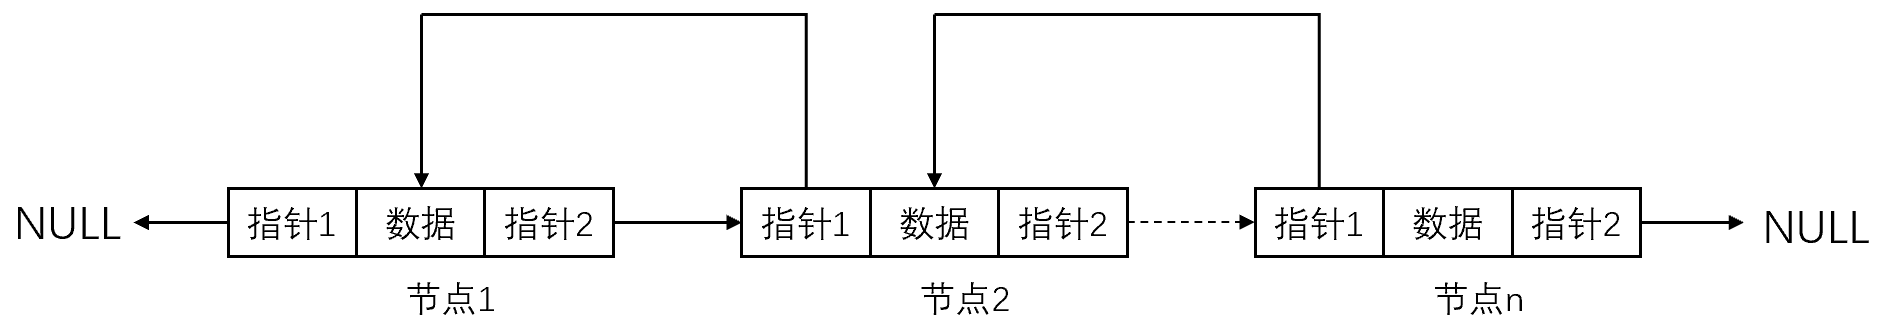
\includegraphics[width=0.78\textwidth]{assets/pics_and_ppts/ch2/双链表示意图.png}
    \caption{双链表示意图}
    \label{fig:双链表示意图}
    
\end{figure}

这样，我们就能以O(1)时间立即找到某个给定节点的前驱节点。同时新增的节点也带来的编码上的不同，比如，在插入、删除节点时，要多维护一个指针（一个很有趣的事实是，你以为
这是让编码更加复杂，但实际上是更加简单。相信在你填充了代码\ref{code:双链表的插入操作}和代码\ref{code:双链表的删除操作}之后会深有体会）。
\begin{thinkbox}
    双链表可不可以带头节点？若不能，为什么？若可以，带头结点会有和单链表类似的好处吗？\\
    双链表的以下操作时间复杂度是多少？\\
    1. 插入操作；2. 删除操作； 3. 按位序访问； 4.按值访问； 5. 求表长。
\end{thinkbox}
正如笔者一再指出，对《数据结构》的研究和学习应该是“重在培养能力”。大家通过前面的研究，熟悉了单链表的思想之后，
应该能较轻松地写出双链表相关操作的代码。因此，笔者在这里进行第一次“留白”，请大家自行实现双链表操作的代码，并分析时间空间复杂度。

\minisection{1.双链表的插入操作}
时间复杂度：$\underline{\hspace{1cm}}$，空间复杂度：$\underline{\hspace{1cm}}$。
\begin{cppcodeNum}[label={code:双链表的插入操作}, codetitle={双链表的插入操作}, showlinenumber=false]
// 在双链表L中，第index个位置插入一个值为e的元素. DL: Double Linked.
    void DLListInsert(ListNode* L, int index, ElemType e) {
        












    }
\end{cppcodeNum}
\minisection{2.双链表的删除操作}
时间复杂度：$\underline{\hspace{1cm}}$，空间复杂度：$\underline{\hspace{1cm}}$。
\begin{cppcodeNum}[label={code:双链表的删除操作}, codetitle={双链表的删除操作}, showlinenumber=false]
// 在双链表L中，删除第index位置的元素。
    void DLListDelete(ListNode* L, int index) {
        
    











    }
\end{cppcodeNum}

这里笔者仅提示一点：我们在\ref{subsec:插入和删除}曾经指出，在已经拿到待删节点指针的情况下，单链表的删除操作的时间复杂度仍然为O(n)。但是双链表却不同，在已经
拿到待删节点指针的情况下，可以达到O(1)的时间复杂度。

\subsection{循环链表}
如果让单链表的表尾节点的后继指针指向表首节点，而不是NULL，这就成为了一个\term{循环单链表}，如图\ref{fig:循环链表示意图} a）；类似地，
将双链表的表首节点的前驱指针指向表尾节点，同时将表尾节点的后继指针指向表首节点，而不是NULL，就成为了\term{循环双链表}，如图\ref{fig:循环链表示意图} b）。
\begin{figure}[htbp]
    \centering
    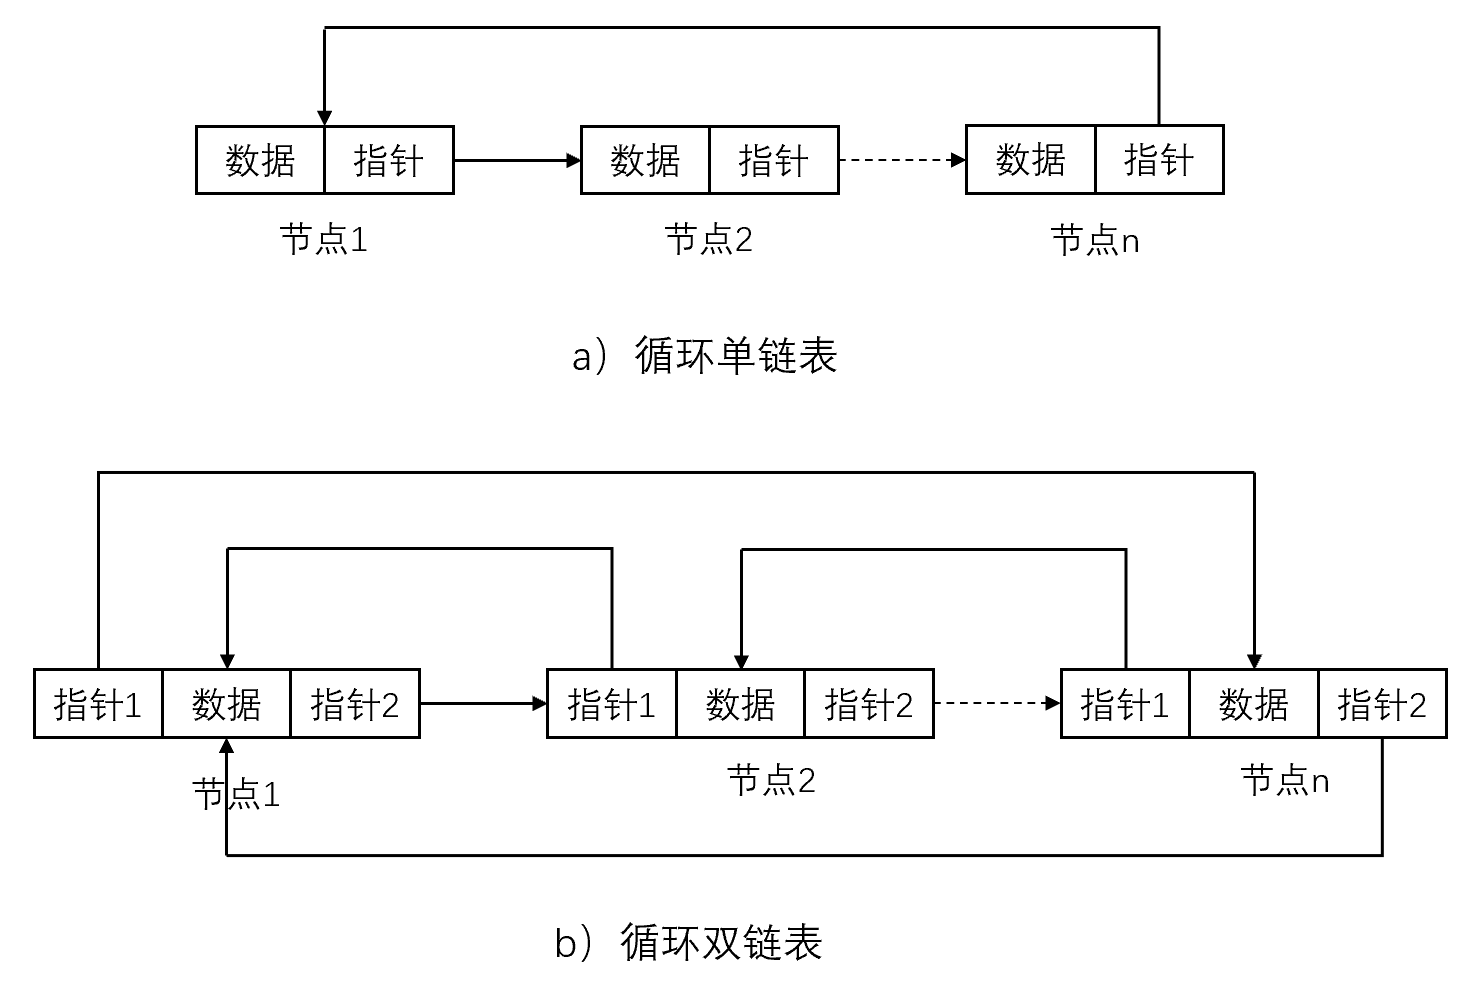
\includegraphics[width=0.78\textwidth]{assets/pics_and_ppts/ch2/循环链表示意图.png}
    \caption{循环链表示意图}
    \label{fig:循环链表示意图}
\end{figure}
可以看出，循环链表由于其循环的特性，给出其任一位置的指针，都可以顺着该指针遍历链表。在这里，我们指出两点循环链表带来的好处。

1. 与普通双链表相比，循环双链表可以在O(1)时间完成尾插。

2. 事实上对于循环单链表来说，保存尾指针（而不是头指针）通常是一种更好的做法，因为有了尾指针p，即可以通过p->next立即找到头指针。并且保存尾指针的循环单链表在
表头和表尾插入元素都可以在O(1)时间实现。

\subsection{静态链表}
实际需求中，有些场景需要频繁地创建、销毁对象，如某空战游戏，战机频繁地打出子弹，子弹碰撞到某物体后或飞出屏幕外之后消失。这种场景下，如果我们频繁地调用
malloc/free就会产生较严重的内存分配开销以及内存碎片（相信如果你学习过《操作系统》就会对此有深刻理解）。这种场景：1. 普通链表非常适合频繁插入删除，
但链表的动态节点分配机制，在高频创建/销毁场景下带来了额外开销； 2. 顺序表又不适合频繁地插入删除。

所以这个时候，\term{静态链表}就可以派上用场。如图\ref{fig:静态链表示意图}所示，静态链表将链表中的所有节点存放在一个数组中。使用数组中的位置编号（下标）
来模拟指针，从而实现节点之间的链接关系。对于单链表，若某节点的后继指针指向NULL说明该节点是表尾节点。而静态链表，通常用一个不存在的下标（如-1）表示没有下一个节点了。
\begin{figure}[htbp]
    \centering
    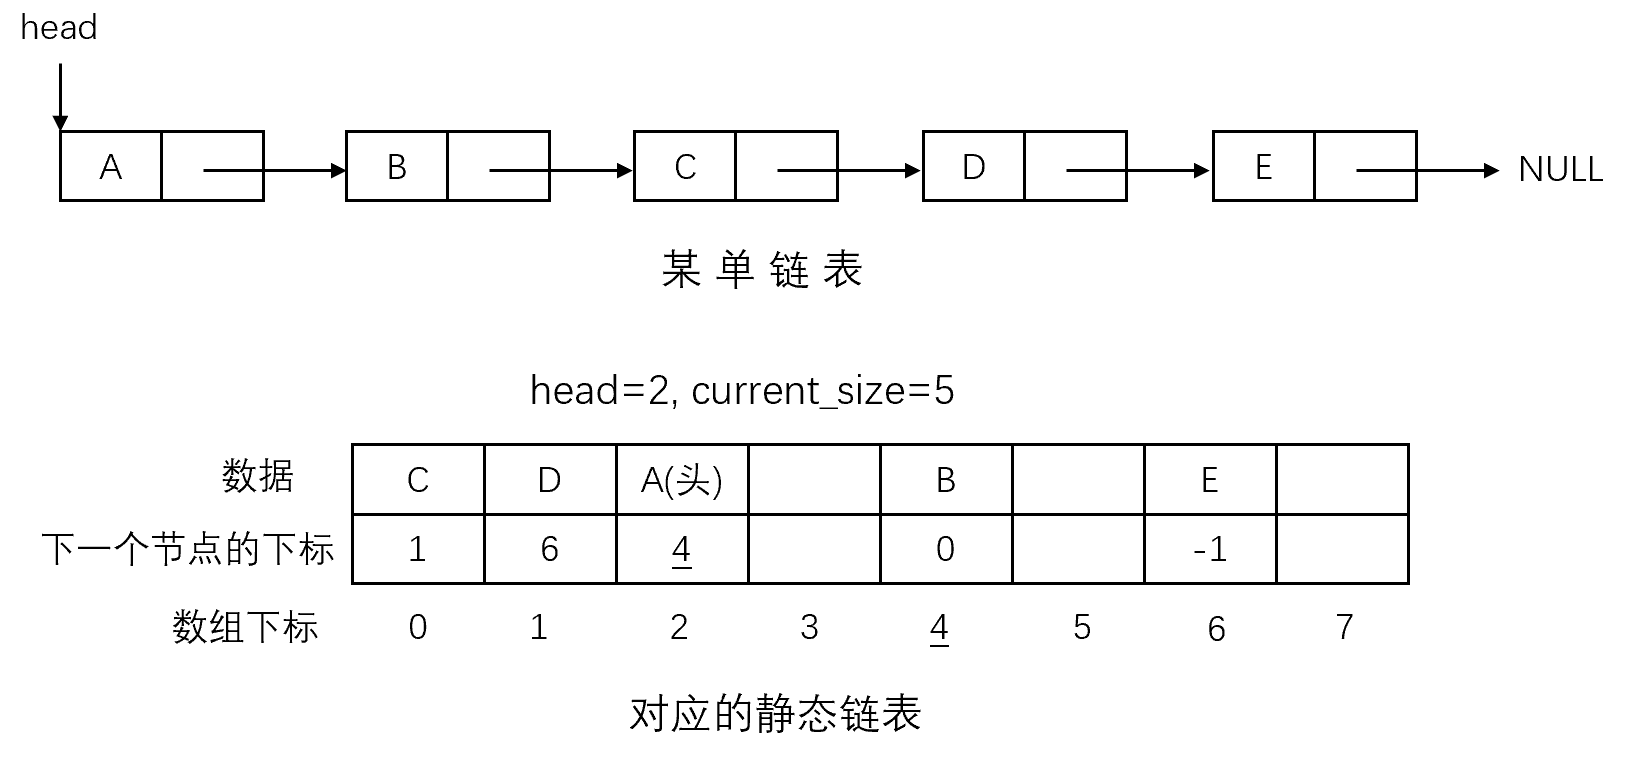
\includegraphics[width=0.78\textwidth]{assets/pics_and_ppts/ch2/静态链表示意图.png}
    \caption{静态链表示意图}
    \label{fig:静态链表示意图}
\end{figure}

静态链表的一个节点的存储结构如以下代码所示：
{
\setminted[cpp]{texcomments=true}
\begin{cppcodeNum}[label={code:静态链表的节点定义}, title={静态链表的节点定义}, minted options app={texcomments}]
    typedef struct {  
        ElemType data;  // 对应图 \ref{fig:静态链表示意图} 中的“数据”
        int next_node;  // 对应图 \ref{fig:静态链表示意图} 中的“下一个节点的下标”
    }SLinkListNode;
\end{cppcodeNum}
}

普通链表可以用其第一个节点的指针表示链表对象，对于静态链表，如何知道数组中哪个节点是第一个节点呢？一种做法是进行类似如下的封装：
\begin{cppcode}
    struct SLinkList {
        SLinkListNode data[MaxSize];    // 存放链表中节点的数组
        int current_size;   // 当前链表中的节点数量
        int head;   // 第一个节点所在的下标 
    }
\end{cppcode}
这样，我们便可以通过如下代码初始化一个静态链表：
\begin{cppcode}
    SLinkList L;
    L.current_size = 0;
    L.head = -1;    // 目前是空表 
\end{cppcode}
静态链表的其他操作，感兴趣的同学可以自行尝试实现。

\section{本章小结}
“\term{数据结构}是相互之间存在一种或多种特定“关系”的数据元素的集合，以及定义在这些数据元素上的“操作”的集合。“数据结构”的物理存储、操作通常通过计算机语言来实现。”
相信通过本章的探讨，大家已经能进一步理解这句话的含义。“线性表”作为一种逻辑结构，要求数据元素之间有“位置关系”，每个节点（除表尾节点）有且仅有一个直接后继，每个
节点（除表首节点）有且仅有一个直接前驱。而顺序表和链表是线性表的两种不同实现方式，分别将线性表的元素以不同的物理结构存储，并通过不同手段建立元素间的逻辑关系。

\term{笔者再次强调}，研究数据结构的核心，并不是掌握某一种数据结构的代码，而是理解如何组织数据、如何分析问题、如何设计解决方案。以链表为例，我们学习的并不仅仅是：

-  链表的定义是什么；

-  链表有哪些操作；

-  创建一个结点的代码是什么； 

-  插入和删除操作的代码是什么； \\
更重要的是理解：

-  为什么需要链表的存在，它能解决什么问题？

-  为什么链表不需要连续的存储空间； 

-  为什么它能够高效地完成插入和删除；   

-  为什么它无法像数组一样快速随机访问； 

-  如何根据问题特点，在灵活性和效率之间进行选择。 \\
因此，学习数据结构时，不要只关注“这个结构怎么实现”（虽然这固然重要），而更应该思考：

-  为什么要这样设计？

-  它解决了什么问题？

-  它付出了什么代价？

-  如果换一种设计，会发生什么变化？\\
当你能够从这些角度理解一个数据结构时，你掌握的就不再只是链表、栈、队列或者树，而是一种分析问题和设计方案的能力。
这也是学习数据结构最重要的意义。

\chapter{栈和队列}
先说栈。在实际应用中有很多类似栈的数据调度方式。想象冬天你去澡堂洗澡。你脱衣服的顺序一定是从外到内，而穿衣服刚好相反。如图\ref{fig:洗澡穿脱衣服的例子}。
\begin{figure}[htbp]
    \centering
    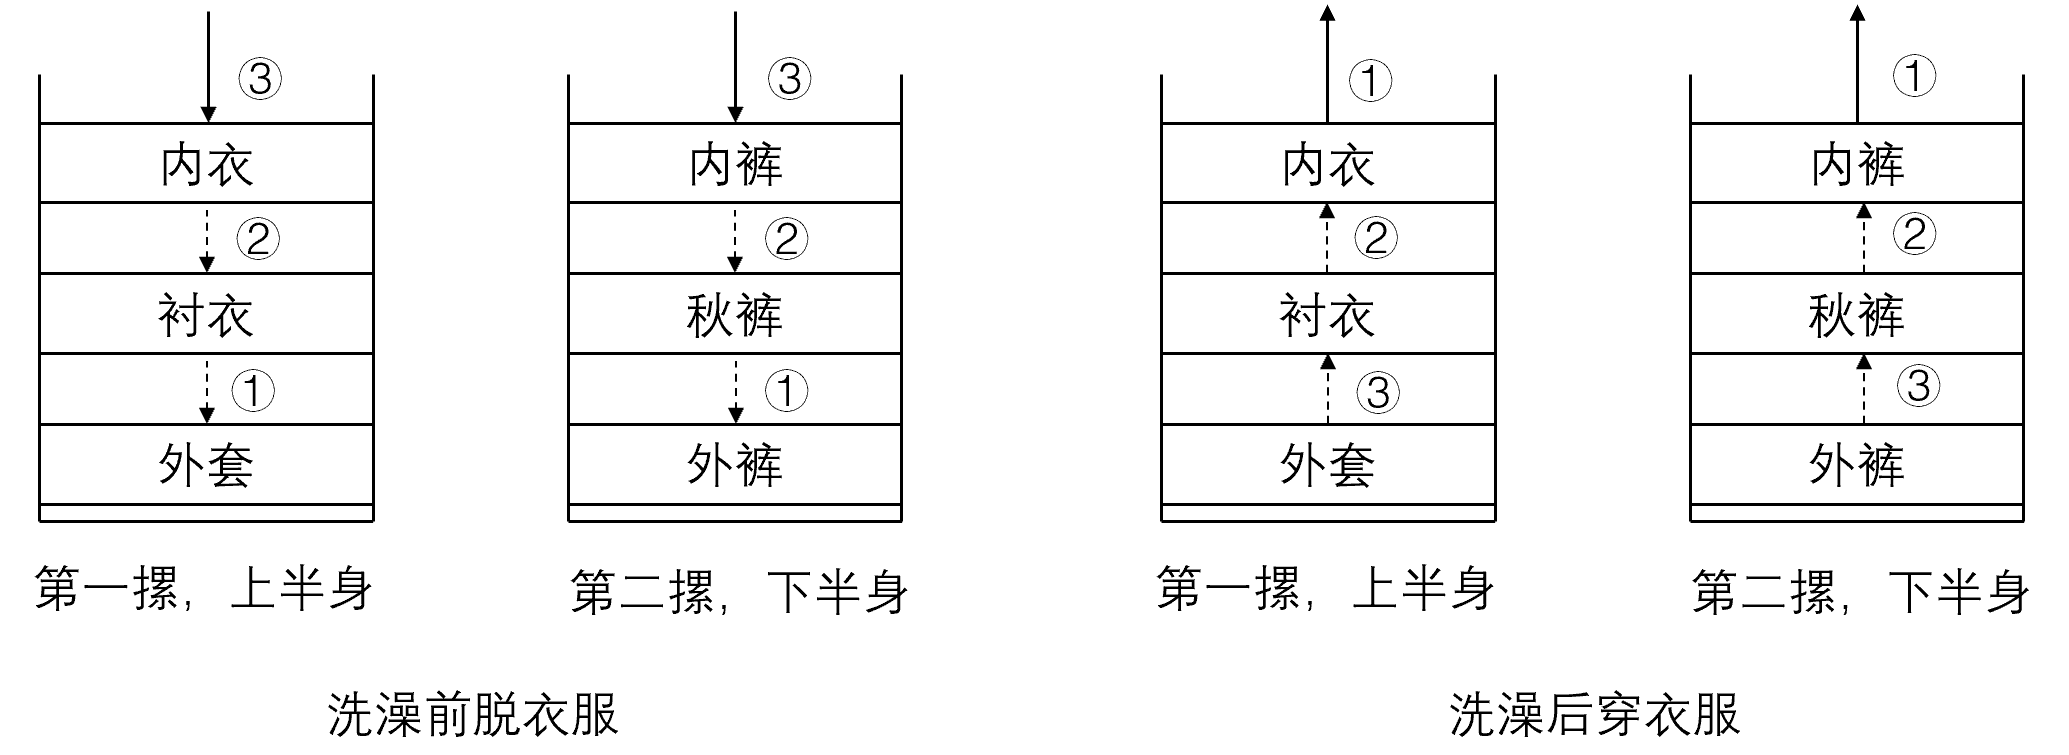
\includegraphics[width=0.78\textwidth]{assets/pics_and_ppts/ch3/洗澡穿脱衣服的例子.png}
    \caption{}
    \label{fig:洗澡穿脱衣服的例子}
\end{figure}

事实上，如果你将两摞衣物放在某个容器里，你会发现这个容器有这样的特点：先放入的在下方，后取出；后放入的在上方，先取出，称为\term{“后进先出”}，或者叫\term{“先进后出”}。
这样，其实你就是在将这两个容器当成两个\term{栈}来使用。\\


而\term{队列}就很好理解了，正得名于生活中的“队列”。想象某门店很火爆，门前排满了人，\uwave{队首}的人买完东西\uwave{出队}，新来的人\uwave{入队}到队尾。

接下来我们给出完整、严谨的\uwave{栈}和\uwave{队列}的定义。

\begin{definitionbox}
    \term{栈（Stack）}是只允许在一端进行插入或删除操作的\uwave{线性表}。
\end{definitionbox}
如图\ref{fig:栈的示意图}所示，允许插入或删除的那一端叫做\term{栈顶}，不允许插入或删除
的另一端叫做\term{栈底}，不包含任何元素的空表叫做\term{空栈}。栈的插入操作叫做\term{入栈}，删除操作叫做\term{出栈}，入栈和出栈通常也更生动地叫做“压栈”和“弹出”。
\begin{center}
    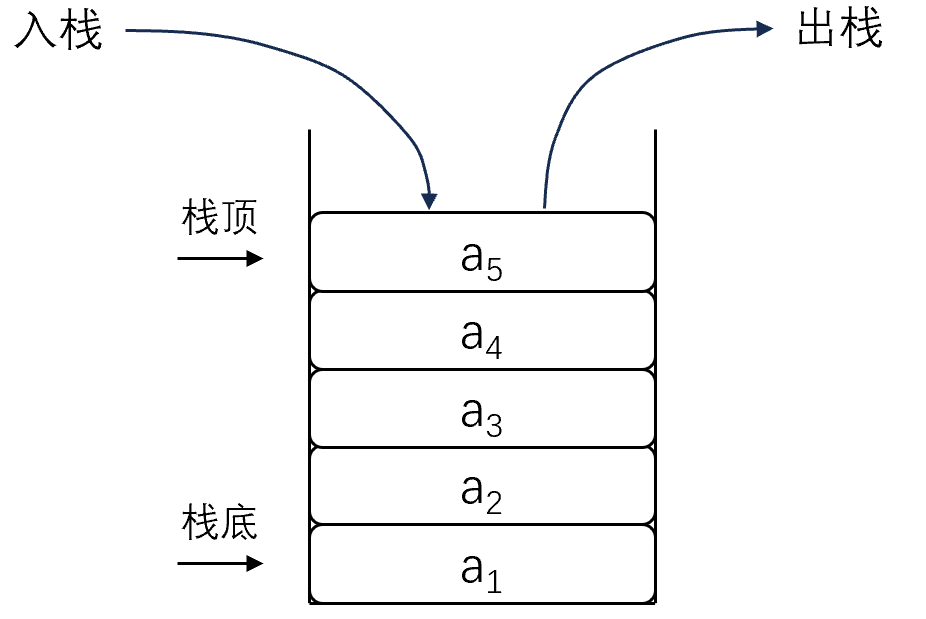
\includegraphics[width=0.48\textwidth]{assets/pics_and_ppts/ch3/栈的示意图.png}
    \captionof{figure}{栈的示意图}
    \label{fig:栈的示意图}
\end{center}

下面给出\term{队列}的定义。
\begin{definitionbox}
    \term{队列（Queue）}是只允许在其中一端插入、另一端删除的\uwave{线性表}。
\end{definitionbox}
如图\ref{fig:队列示意图}所示，允许出队的那一端叫做\term{队首}，允许入队的那一端叫做\term{队尾}，队列的插入操作叫做\term{入队}，删除操作叫做\term{出队}；
不包含任何元素的空表叫做\term{空队列}。
\begin{figure}[htbp]
    \centering
    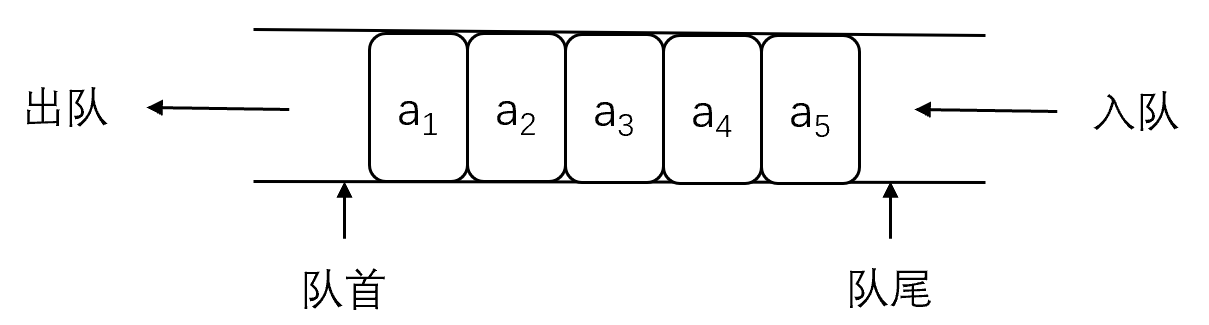
\includegraphics[width=0.55\textwidth]{assets/pics_and_ppts/ch3/队列示意图.png}
    \caption{队列示意图}
    \label{fig:队列示意图}
\end{figure}

很多人喜欢将栈和队列的特征进行对比，称\term{队列是先进先出（First In First Out, FIFO）的，栈是后进先出（Last In First Out，LIFO）的。}

以上便是栈和队列这两种逻辑结构的介绍，接下来我们研究如何实现栈和队列。
\section{栈}
上一章中我们研究了顺序表与链表的实现。既然栈是一种特殊的线性表，是不是可以用同样的物理存储来实现栈，并且对操作加以特殊限制呢？笔者建议大家在这里暂停，思考一下这个问题：
想象一下，分别用数组、链表该如何实现栈？如何设计是好的？会面临哪些问题吗？\\

此处应该有长时间留白......\\

开始。\\

相信大多数人的都会有明确而正确的思路：\\

1. 如果使用顺序表来实现栈，由于顺序表“尾插”、“尾删”均为O(1)的特性，可以将“表尾”作为“栈顶”，通过操作的定义和实现来限制该表
只能在表尾插入、删除，这样既有高效率，又满足栈的特点。如图\ref{fig:顺序栈实现示意图}所示，你可能会想到用一个int型变量top来动态维护“栈顶”的位置。
\begin{figure}[htbp]
    \centering
    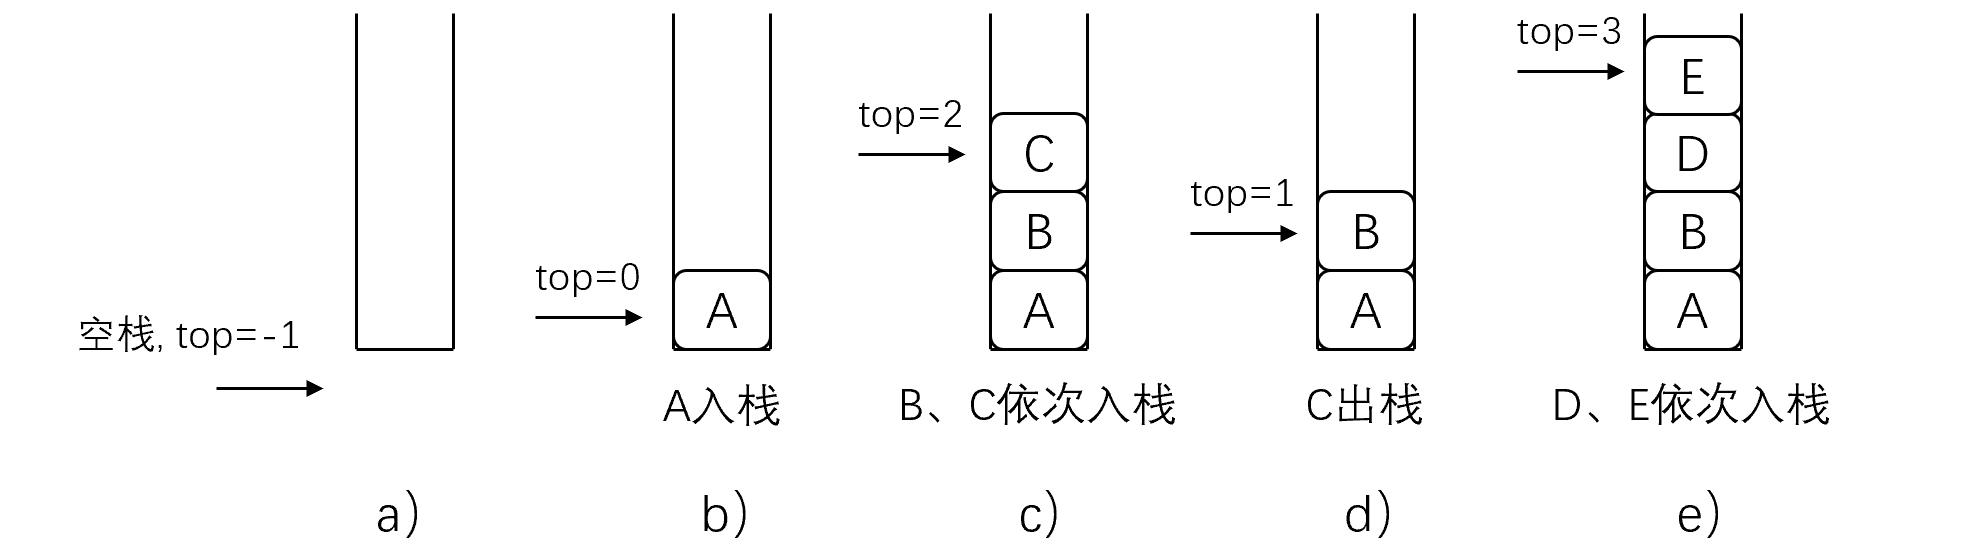
\includegraphics[width=0.78\textwidth]{assets/pics_and_ppts/ch3/顺序栈实现示意图.png}
    \caption{顺序栈实现示意图}
    \label{fig:顺序栈实现示意图}
\end{figure}

这个思路其实就是\term{顺序栈}的实现思路。采用顺序存储的栈称为\term{顺序栈}，它利用一组地址连续的存储单元存放自栈底到栈顶的数据元素，同时附设一个指针top，来
指示当前栈顶的位置。

顺序栈的存储结构如以下代码所示：
\begin{cppcode}
    #define MaxSize 100
    struct SeqStack {
        ElemType data[MaxSize]; // 存储实际的数据元素
        int top;    // 栈顶指针的下标
    };
\end{cppcode}
\begin{insightbox}
    你也许会发现，这特么不就是线性表么？你不就把current\_size换成top了么？没错，顺序栈和顺序表的关系确实有点暧昧不清。从存储结构角度看，二者存储结构完全相同，
    只不过语义不同：top表示栈顶元素的下标，空栈时为-1；而current\_size表示顺序表中元素的数量，空表时为0。二者之间微妙的关系在于，current\_size在数值上等于
    表尾元素（栈顶元素）的下标加一。而如果你将top的语义规定为“表尾元素（栈顶元素）的下一个位置”，那么就应将top初始化为0，而不是-1，此时top与current\_size
    语义虽然不同，但编码上是相同的。
\end{insightbox}



2. 如果使用链表来实现栈，由于链表“头插”、“头删”均为O(1)的特性，可以将“表头”作为“栈顶”，通过操作的定义和实现来限制该表
只能在表头插入、删除，这样同样既有高效率，又满足栈的特点。事实上，将链表的插入和删除操作限制在头部，即得到了\term{链栈}。

接下来我们分别给出顺序栈和链栈常见操作的实现。

\subsection{顺序栈的常见操作实现}
\minisection{1.顺序栈的初始化}
不难看出，初始化一个顺序栈仅需要将其栈顶指针top置为-1。
\begin{cppcode}
    int InitStack(SeqStack* S) {
        S.top = -1;
        return 1;
    }
\end{cppcode}
对于一个未初始化的顺序栈S:
\begin{cppcode}
    SeqStack S;
\end{cppcode}
就可以通过以下代码对S进行初始化：
\begin{cppcode}
    InitStack(S);
\end{cppcode}

\minisection{2.进栈操作}
top指针指向“当前栈顶元素”，因此进栈时要先移动指针到下一个“更高的”可用位置，再将元素放入该位置，此时指针仍指向栈顶。
\begin{cppcode}
    int Push(SeqStack& S, ElemType e) {    
        if(S.top == MaxSize - 1) {
            return 0;   // 栈已满，无法入栈
        }
        S.top += 1;
        S.data[S.top] = e;
        return 1;
    }
\end{cppcode}
如以下代码便可以为栈S压入一个值为3的元素：
\begin{cppcode}
    Push(S, 3);
\end{cppcode}

\begin{notebox}{初见提示}
    注意这里我们首次使用了C++的引用作为函数形参。"SeqStack\& S"中，符号"\&"并不是取地址的意思，而是表示形参S是一个SeqStack的\term{引用}类型。相信你也看出引用的作用了，
    类似使用指针一样，使用引用作为形参，同样可以改变函数栈外的原变量的值。关于引用的更多内容感兴趣的同学可以参考C++相关资料。
\end{notebox}

\minisection{3.出栈操作}
思想类似进栈，此处留白，请大家自行写出代码。
\begin{cppcode}
// 将栈S中当前的栈顶元素赋值给e，并将其弹出。
    int Pop(SeqStack& S, ElemType& e) {
        





    }
\end{cppcode}
\minisection{4.获取栈顶元素，但不出栈}
略。

\minisection{5.判断栈是否为空}
\begin{cppcode}
    int Empty(SeqStack S) {
        if(S.top == -1) return 1;   // Empty成立
        return 0;
    }
\end{cppcode}

\subsection{链栈的常见操作实现}
根据前面的介绍相信你已经看出来了，链栈的实现比链表还要简单：其他操作和链表几乎完全相同，而对于“插”和“删”，你只实现链表的“头插”和“头删”操作，而不实现任意位置的插入删除操作，你就得到了一个链栈。
显然链栈也可以采用带头结点和不带头结点的实现。这里拟采用带头结点的实现。

\begin{notebox}{提示}
    对于带头结点的实现，链表的第一个节点指针L指向头节点，L->next\_node指向的是第一个数据元素，即栈顶元素。
\end{notebox}

\minisection{1.链栈的入栈操作（实际上就是链表的“头插”操作）}
\begin{cppcode}
    int Push(ListNode* L, ElemType e) {
        ListNode* new_node = (ListNode*)malloc(sizeof(ListNode));
        new_node->data = e;
        new_node->next_node = L->next_node;
        L->next_node = new_node;
        return 1;
    }
\end{cppcode}

\minisection{2.链栈的出栈操作（实际上就是链表的“头删”操作）}
\begin{cppcode}
    int Pop(ListNode* L, ElemType& e) {
        if(L == NULL || L->next_node == NULL) {
            return -1;  
        }
        e = L->next_node->data;
        ListNode* node_to_free  = L->next_node;
        L->next_node = L->next_node->next_node;
        free(node_to_free );
        return 1;
    }
\end{cppcode}
显然实现一个栈没有必要使用双链表，更没有必要将首尾链接起来做成循环链表。

由于顺序栈和链栈就是有特殊限制的顺序表和链表，其优劣我们不再赘述，而是作为习题放在{\color{red}\textbf{习题2}}中。

\subsection{*浏览器的前进后退功能实现}
这里给出一个作为思维训练、理解栈的意义的极好的例子。大家应该都用过浏览器的“后退”和“前进”功能，如图\ref{fig:浏览器的前进后退示意}。当你按住鼠标右键从右向左滑动，
或者点击右键选择“后退”时，浏览器会访问你上一个访问过的网页，向右滑或点“前进”则回到上一个回退前的网页（如果你没用过，建议先打开浏览器试一下）。
\begin{figure}[htbp]
    \centering
    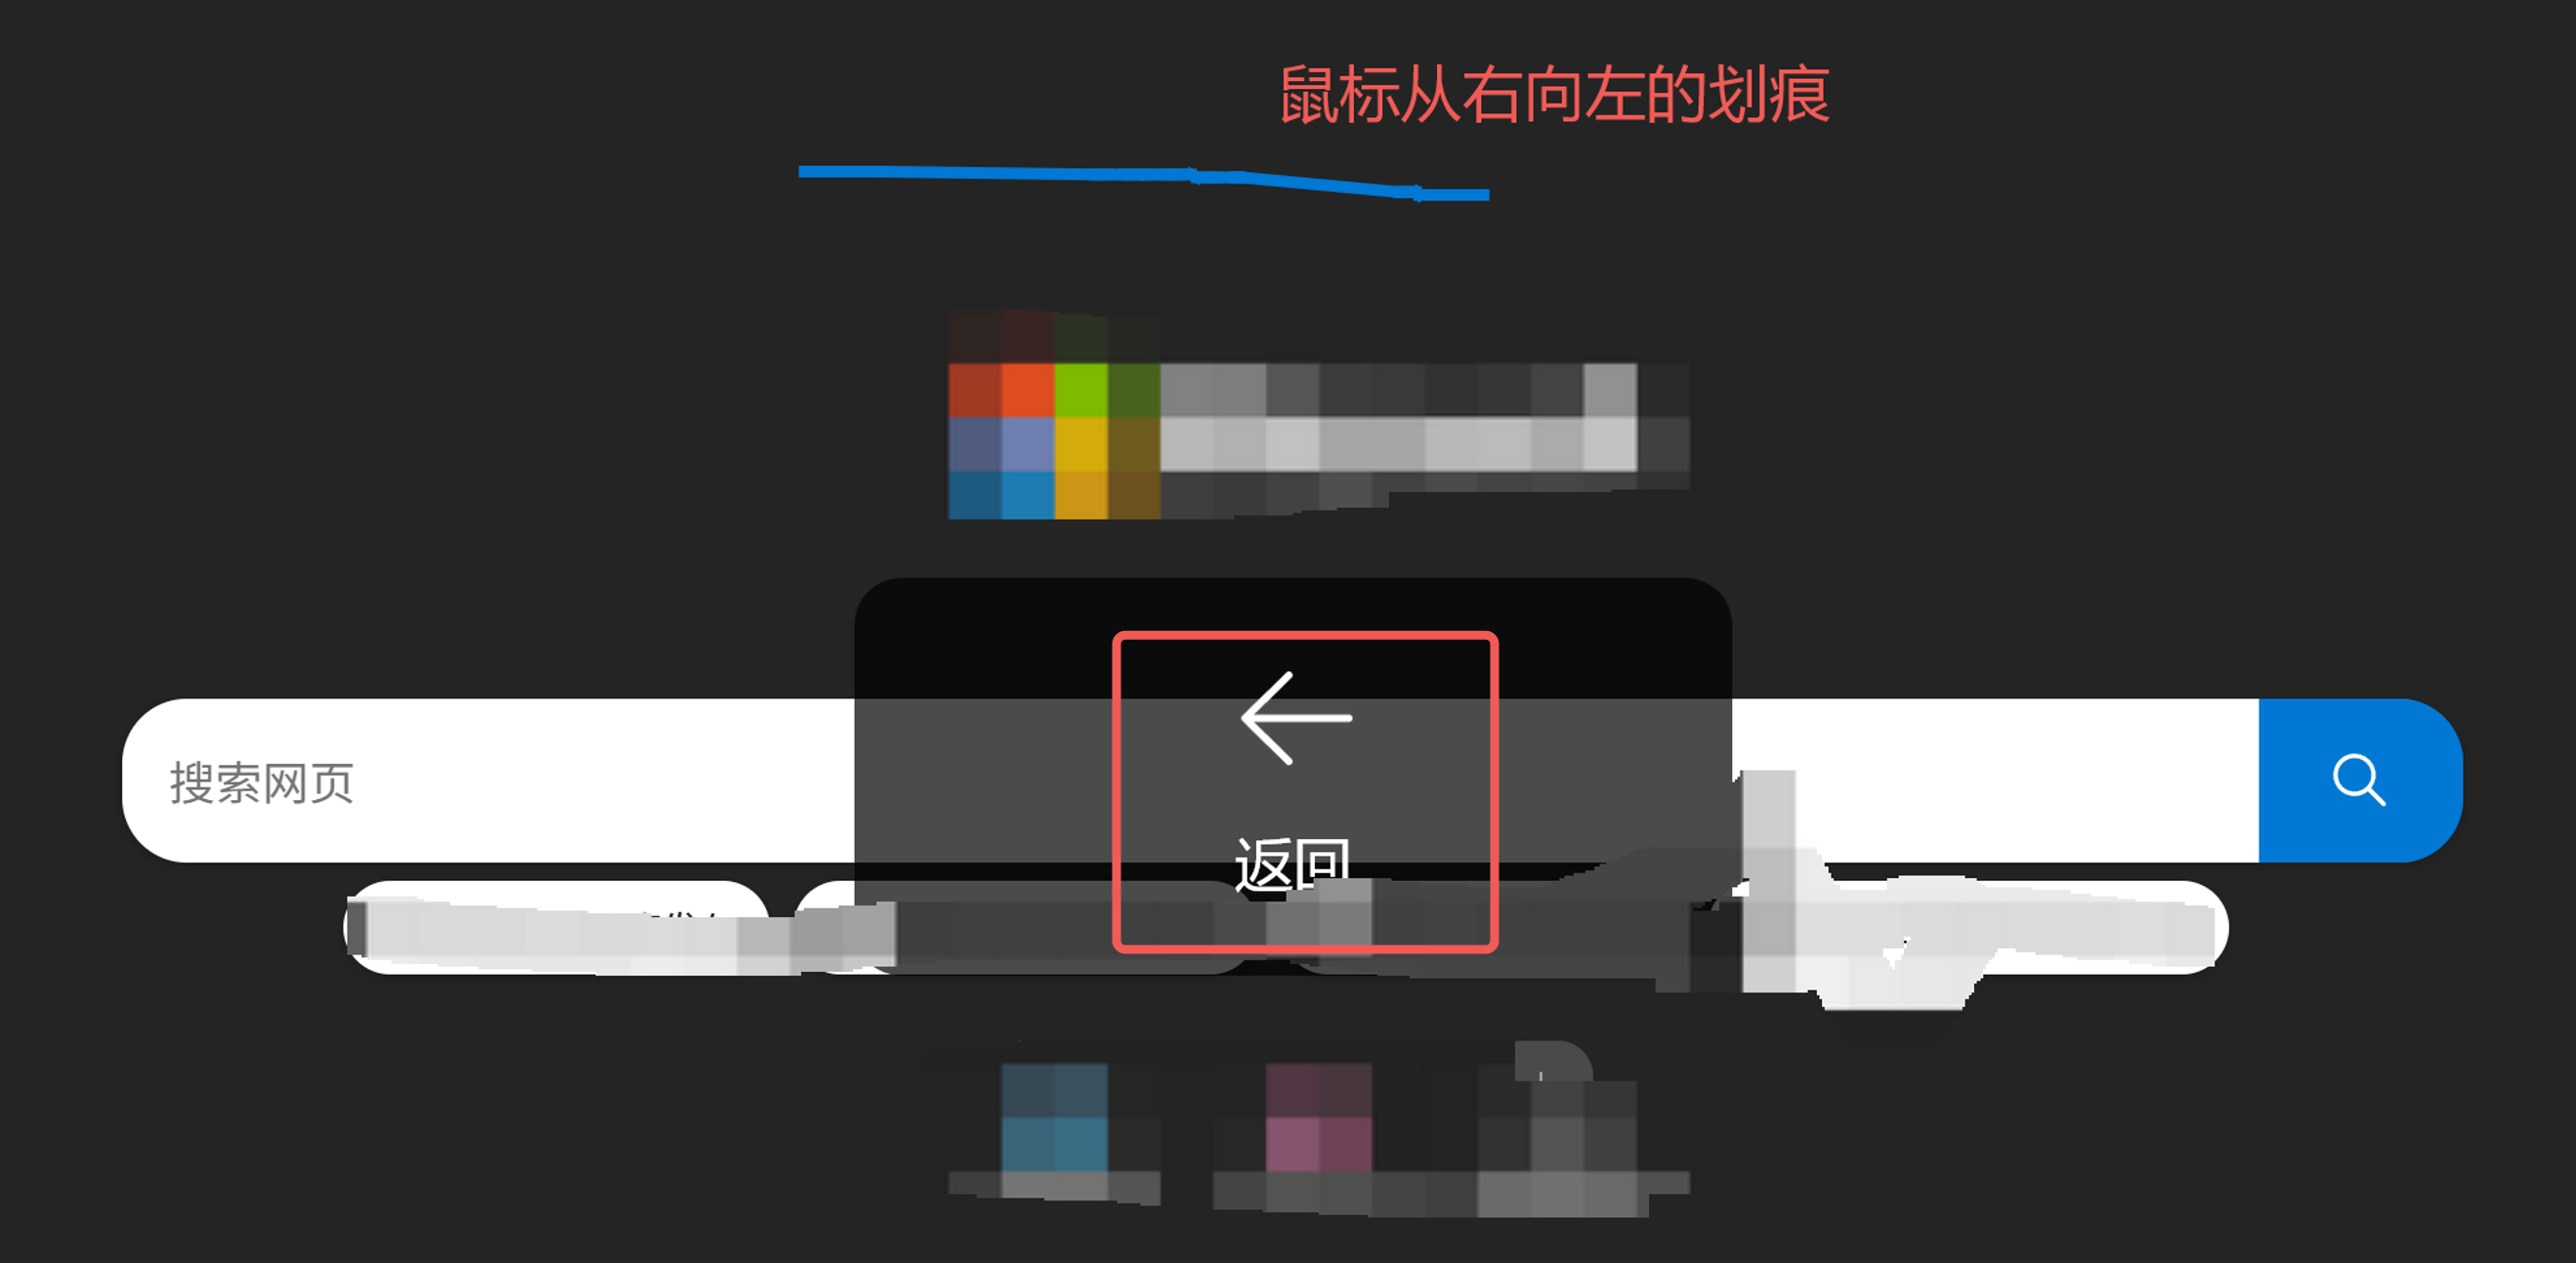
\includegraphics[width=0.6\textwidth]{assets/pics_and_ppts/ch3/浏览器的前进后退示意.png}
    \caption{}
    \label{fig:浏览器的前进后退示意}
\end{figure}
假设你已经访问过了：
\begin{bulk}
    网页1 -> 网页2 -> 网页3 
\end{bulk}
此时你处在网页3，点击“后退”，会回到网页2，再后退，回到网页1，再前进，回到网页2，再前进，回到网页3。

假设：\\
1.用户随时可能访问一个新的网站；\\
2.用户随时可能点击“后退”（鼠标左滑）；\\
3.用户随时可能点击“前进”（鼠标右滑）。\\
如果你是某浏览器的实现者，请你实现这个功能，要求当用户点击“前进”或“后退”时，能迅速地拿到对应网页的地址。

提示：网页地址（如https://xxxxxx）可以用一个char的数组（或string类型）来表示。你可以用任何你喜欢的方式来模拟用户的输入，并让你的程序做出合理反应。\\

此处应该有留白。\\

具体的模拟方式各有千秋，我们只给出核心算法的实现思路。不难看出，当用户访问了若干页面之后：
\begin{bulk}
    网页1 -> 网页2 -> 网页3
\end{bulk}
“后退”操作实际上就是依次访问与之前的顺序相反的页面，满足“后进先出”的特点，因此用户每访问一个\uline{新网页B}，我们就可以将用户所处在的\uline{当前网页A}
压入一个栈back\_stack，当用户进行后退时，取出栈顶网页访问即可。back\_stack语义上可以理解为：为用户的后退行为而预备的一个栈，栈顶元素永远是
用户此时点击后退时所要访问的页面。

还有前进操作。“后退”的顺序是与用户主动访问的新网页顺序相反，不难看出，“前进”的顺序是与“后退”相反的。因此可以维护令一个栈forward\_stack，用户未进行过后退操作时该
栈为空，当用户连续进行“后退”时，将网页依次压入栈forward\_stack。需要注意：当用户访问了一个新网页后无法“前进”，需要清空forward\_stack重新期待用户的下一次后退操作。
流程如图\ref{fig:使用两个栈实现浏览器前进后退}所清晰地展示。

\begin{figure}[htbp]
    \centering
    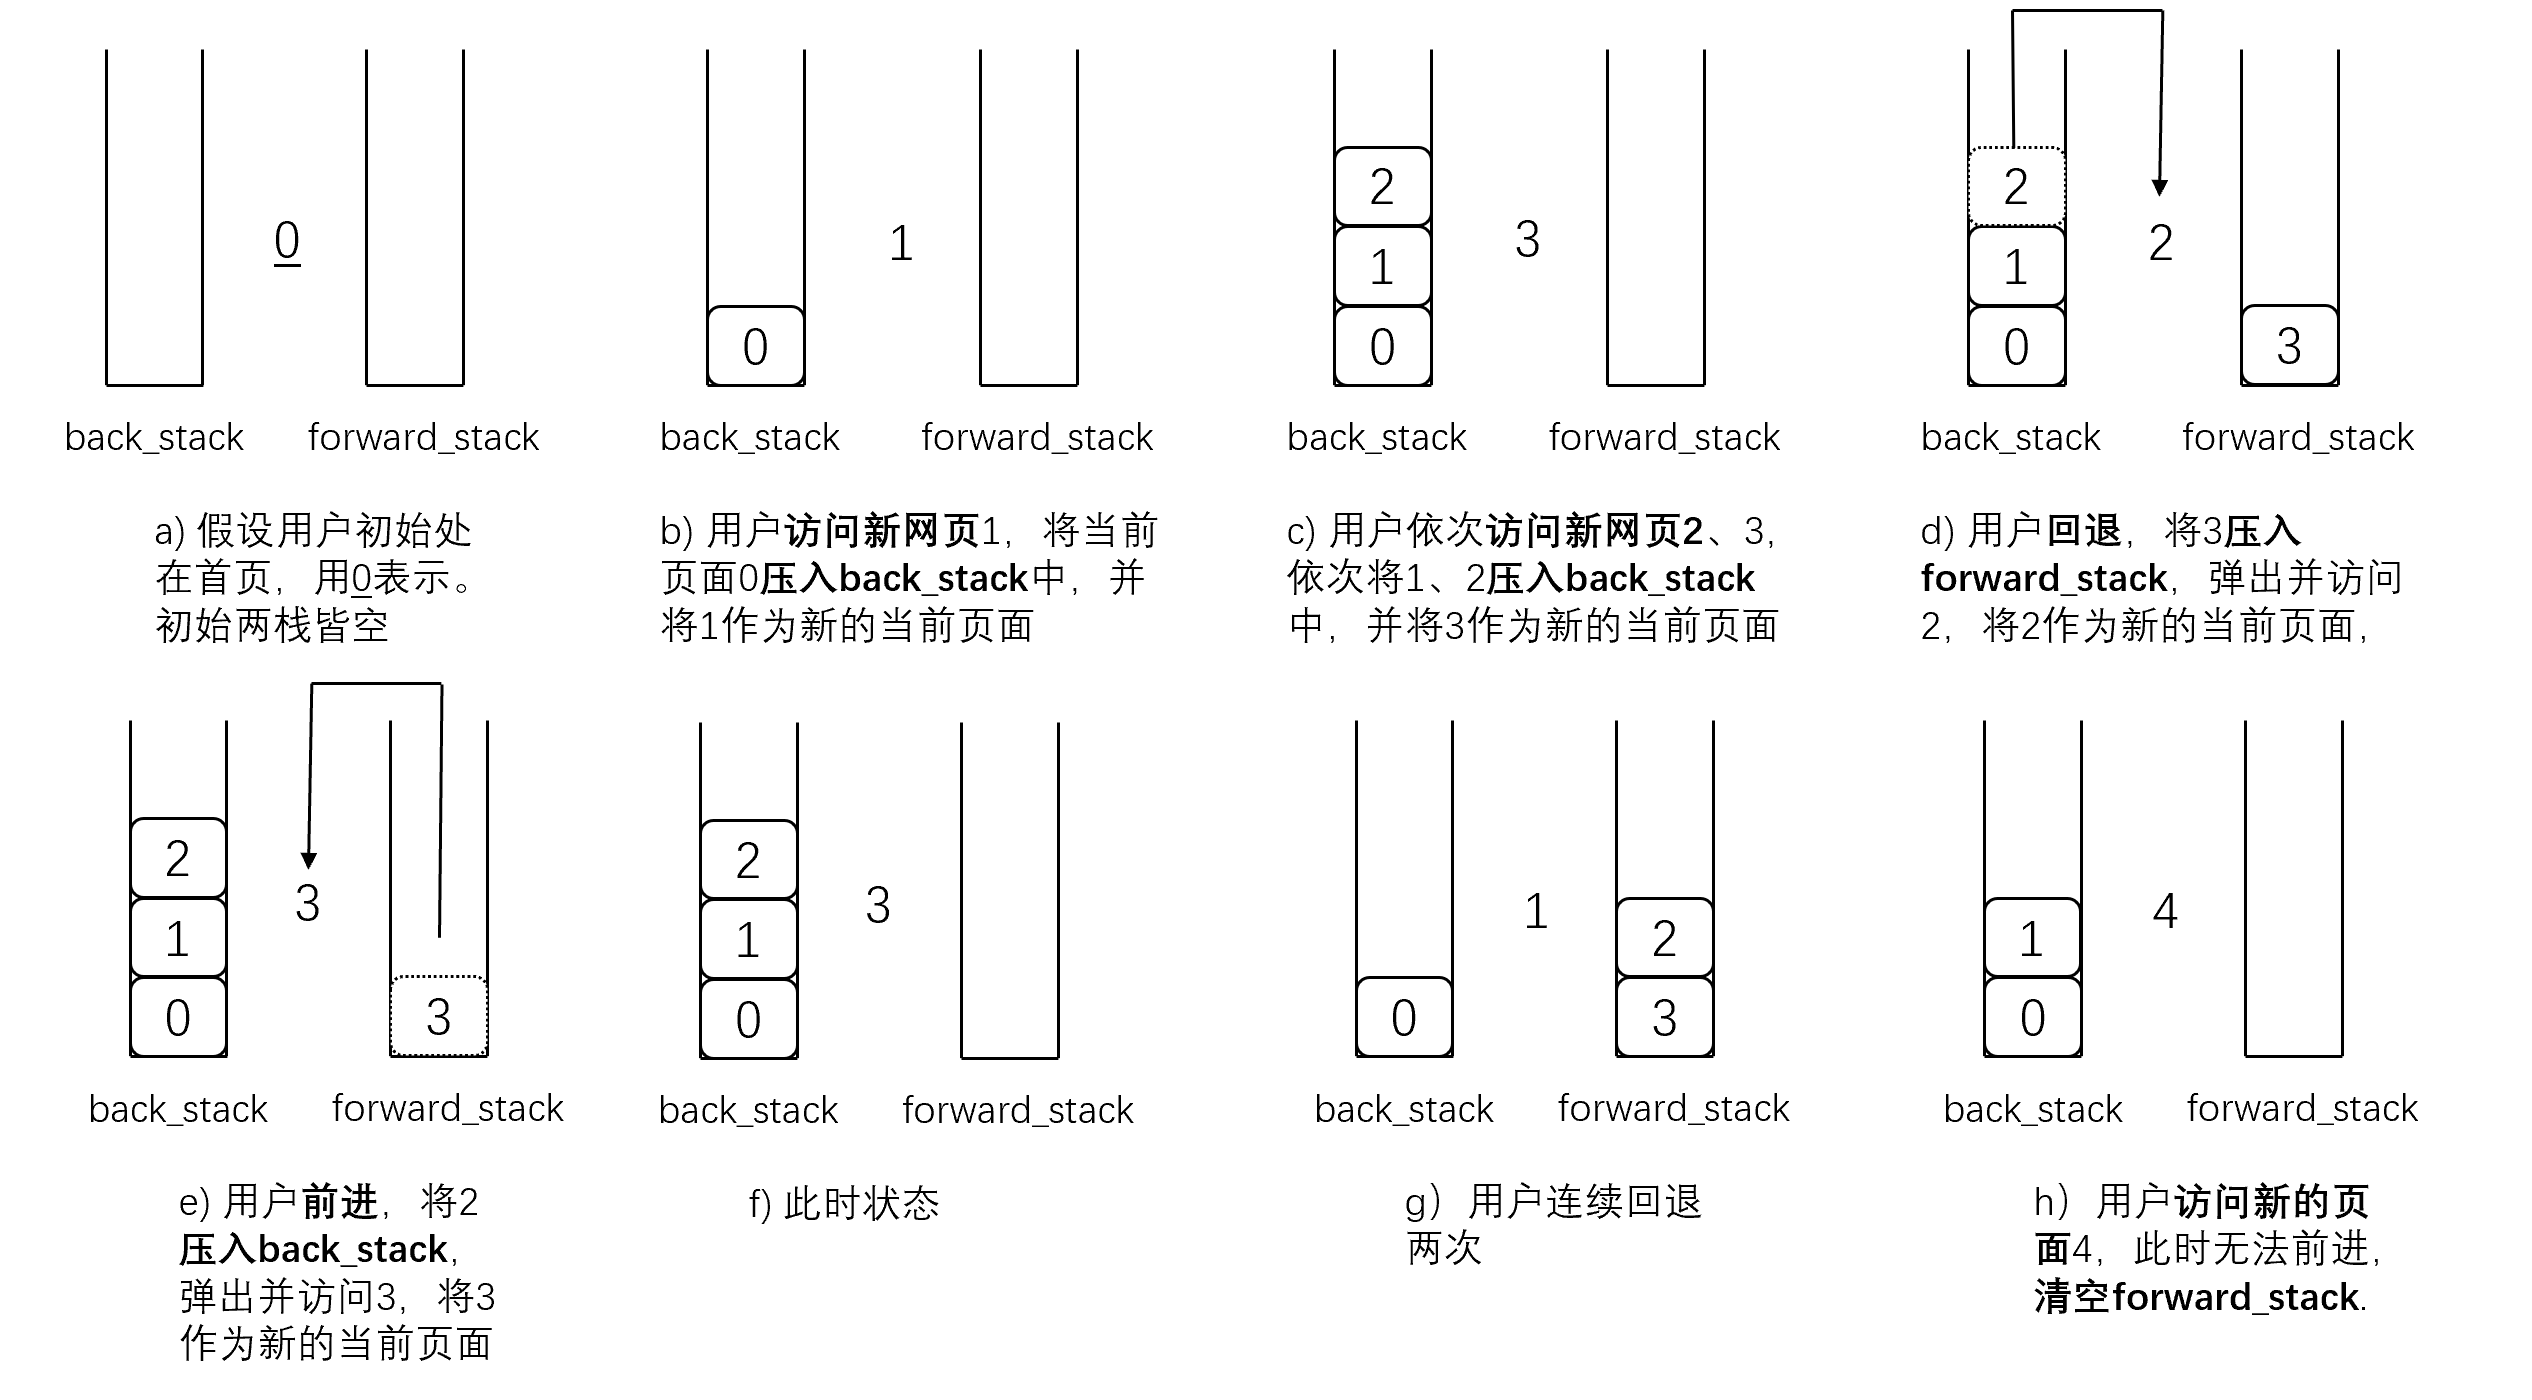
\includegraphics[width=1.15\textwidth]{assets/pics_and_ppts/ch3/使用两个栈实现浏览器前进后退.png}
    \caption{使用两个栈实现浏览器前进后退}
    \label{fig:使用两个栈实现浏览器前进后退}
\end{figure}

\subsection{*“函数栈”、“调用栈”是啥？}
相信大家从未注意但一个很有趣的事实是，函数调用、返回的顺序恰好具有“后进先出（LIFO）”的特点。如：
\begin{cppcode}
    void C() {
        return ;
    }
    void B() {
        C();
    }
    void A() {
        B();
    }
    int main() {
        A();
        return 0;
    }
\end{cppcode}
程序实际执行的顺序是：main -> A -> B -> C -> B -> A -> main -> 退出。函数执行结束时，需要返回上层，因此调用一个新函数时，需要将当前函数的上下文信息压入一个记录“函数调用
记录”的栈中（是不是有点像浏览器？）。从更底层的开发者角度来看，“调用栈”就是存放这些函数信息的一个栈，栈中的每一个元素是相应的函数上下文信息，如函数参数、局部变量
、返回地址等。

但对于应用程序员，特别是C/C++程序员来说，“调用栈”或“函数栈”通常存在其他角度的含义。对于C/C++来说，非静态局部变量存放在栈区，其可访问区域仅在函数内部。如：
\begin{cppcodeNum}[label={code:调用栈示例代码}]
    int f(int t) {
        int a = 10;
        t = t + a;
    }

    int main() {
        int x = 2;
        f(x);
        return 0;
    }
\end{cppcodeNum}
事实上，调用函数时，操作系统通常会为其分配一个栈区空间，其局部变量便存储在这个栈区空间中。main函数中以x为参数调用f(x)，仅仅是将x的值\uwave{拷贝}给了“栈区变量”t。
因此，这种场景下我们常称t是“f的函数栈（或调用栈）中的一个栈变量”，此时“函数栈”或“调用栈”的含义便是内存中的“栈区”空间。

\begin{notebox}{提示}
    事实上，函数的形参可以理解为函数栈中的一个局部变量。如代码\ref{code:调用栈示例代码}，以x为实参调用f，可以等效理解为如下伪代码：
    \begin{cppcode}
        int f() {
            int t;
            t = x;  // 外界传入的x的值拷贝给t
            ...

        }
    \end{cppcode}
    这也进一步解释了值传递无法改变函数栈外的原变量的值，而需要通过指针传递。
\end{notebox}

\section{队列}
如前所述，队列同样是一种特殊的线性表，因此队列同样可以有顺序存储和链式存储两种物理结构，并在顺序表或链表的基础上实现特殊机制。队列的链式存储稍简单些，
我们先研究链式存储，再研究顺序存储。

\subsection{队列的链式存储}
队列需要实现两个操作：在链表的头部删除元素、尾部插入元素。单链表头插本身可以达到O(1)。我们只要额外保存一个链表的尾指针，那么在尾部插入元素的操作也可以达到O(1)。显然
链式队列同样可以带头结点或不带头节点，这里拟采用带头节点的实现。

第二章中已经给出过链表节点的定义，这里为了体现出节点是队列的节点，我们把结构改个名字：
\begin{cppcode}
    struct QueueNode {
        ElemType data;
        struct QueueNode* next_node;
    };
\end{cppcode}
额外保存一个表尾指针来使出队操作时间达到O(1)：
\begin{cppcode}
    typedef struct {
        struct QueueNode* front;     // 表头(队首)指针，指向头节点
        struct QueueNode* rear;     // 表尾(队尾)指针，指向最后一个节点
    }LinkQueue;
\end{cppcode}
以上代码将LinkQueue定义为一个“链队列”类型。有了如上定义，我们就可以用如下代码定义链队列对象：
\begin{cppcode}
    LinkQueue happy_linkqueue;  // 定义一个开心的链队列
    LinkQueue sad_linkqueue;    // 定义一个悲伤的链队列
\end{cppcode}
一个链队列如图\ref{fig:带头结点的链式队列示意图}所示。前面的happy\_linkqueue以及sad\_linkqueue都是定义了但未初始化的。接下来我们给出链式队列的常见操作实现（带头结点）。
\begin{figure}[htbp]
    \centering
    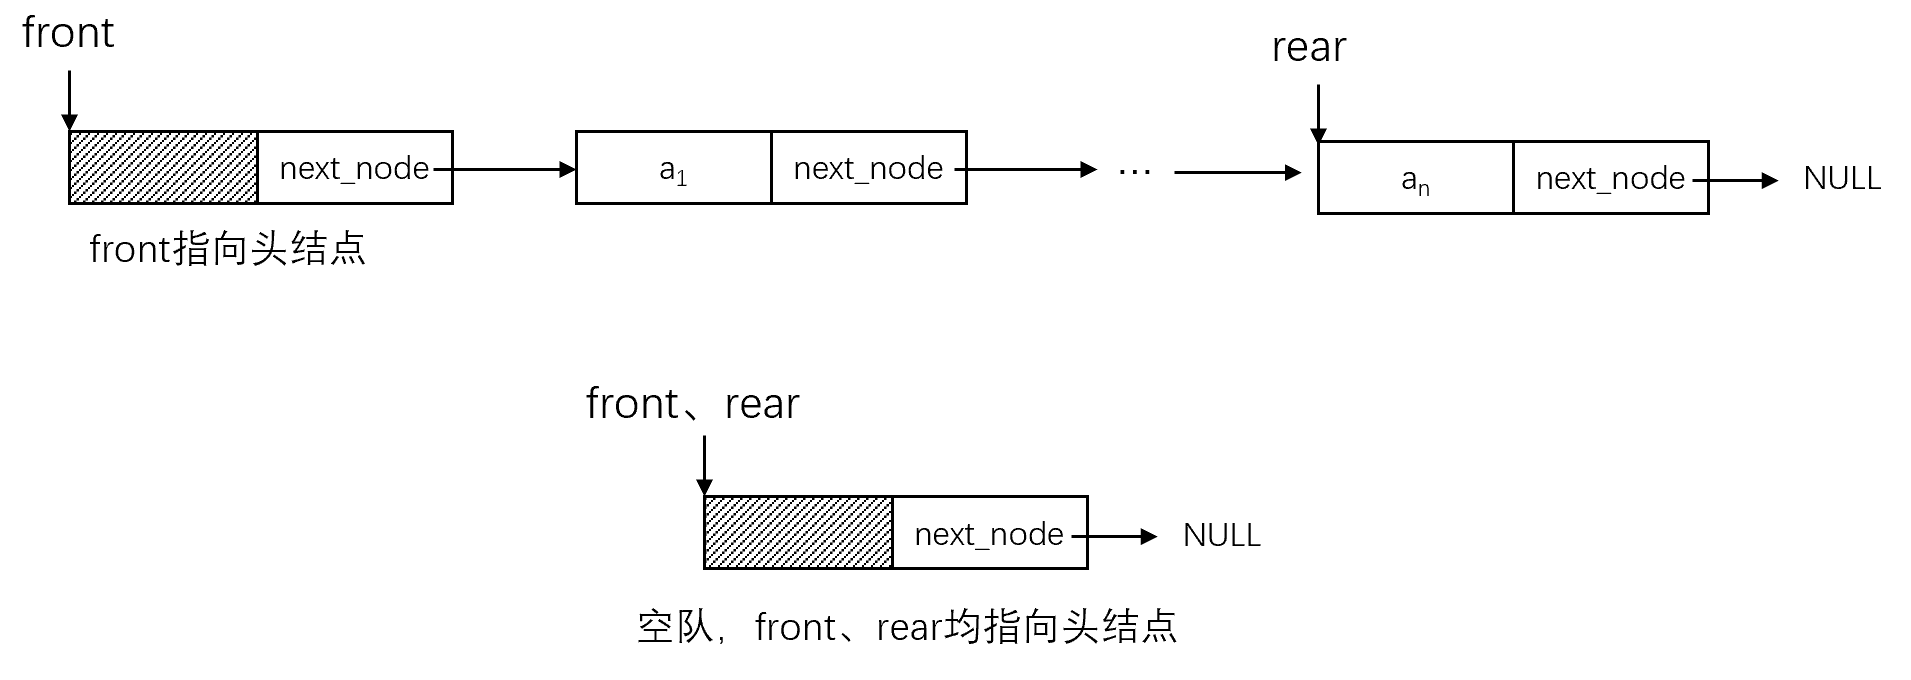
\includegraphics[width=0.85\textwidth]{assets/pics_and_ppts/ch3/带头结点的链式队列示意图.png}
    \caption{带头结点的链式队列示意图}
    \label{fig:带头结点的链式队列示意图}
\end{figure}

\minisection{1.初始化操作}
\begin{cppcode}
    int InitLinkQueue(LinkQueue& q) {
        q.front = (QueueNode*)malloc(sizeof(LinkQueue));     // 为头节点分配空间
        q.rear = q.front;    // 由于插入时要在尾后插入，所以rear初始指向头节点符合条件

        q.front->next_node = NULL;
        q.rear->next_node = NULL;
        return 1;
    }
\end{cppcode}
使用：
\begin{cppcode}
    InitLinkQueue(happy_linkqueue); // 初始化开心的链队列
    InitLinkQueue(sad_linkqueue);   // 初始化悲伤的链队列
\end{cppcode}

\minisection{2.判断是否空队}
\begin{cppcode}
    int Empty(LinkQueue q) {
        if(q.front == q.rear) {
            return 1;
        } 
        return 0;
    }
\end{cppcode}

\minisection{3.入队操作（尾插）}
\begin{cppcode}
    int EnQueue(LinkQueue& q, ElemType e) {
        if(q.front == NULL || q.rear == NULL) {
            return -1;  // 你给我个没初始化的队列我咋给你插入元素？
        }
        QueueNode* nwe_node = (QueueNode*)malloc(sizeof(QueueNode));
        nwe_node->data = e;
        // 操作链条
        nwe_node->next_node = NULL;
        q.rear->next_node = nwe_node;

        // 更新尾指针
        q.rear = nwe_node;
        return 1;
    }
\end{cppcode}

\minisection{4.出队操作（头删）}
一般情况下出队不会改变尾指针的指向，但需要注意一个特殊情况，即队列中仅有一个节点，如图\ref{fig:仅有一个数据节点的队列}所示。此时队首节点就是队尾节点，出队后，
队列变成空队，需要维护队尾节点指针，将其指向头节点。
\begin{cppcode}
    int DeQueue(LinkQueue& q, ElemType& e) {
        if(q.front == NULL || q.rear == NULL) {
            return -1;
        }
        if(q.front == q.rear) {
            return 0;   // 空队
        }   // 注意代码若能走出这个if，说明队中至少有一个数据节点，可以直接安全地访问q.front->next_node的data域或next_node域。
        e = q.front->next_node->data;
        QueueNode* t = q.front->next_node;
        q.front->next_node = q.front->next_node->next_node;

        // 若队列仅有一个节点，更新q.rear
        if(q.rear == t)
            q.rear = q.front;
        }
        free(t);
        return 1;
    }
\end{cppcode}
\begin{figure}[htbp]
    \centering
    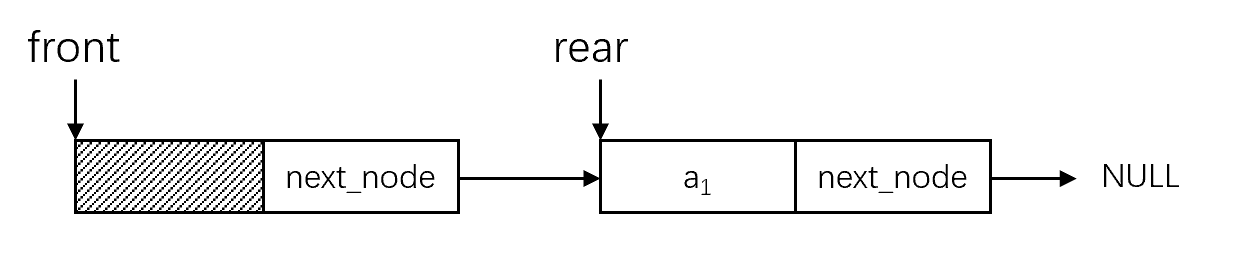
\includegraphics[width=0.70\textwidth]{assets/pics_and_ppts/ch3/仅有一个数据节点的队列.png}
    \caption{仅有一个数据节点的队列}
    \label{fig:仅有一个数据节点的队列}
\end{figure}

\subsection{队列的顺序存储}
不难想到，要在顺序存储的线性表上实现一个队列，最简单的做法就是标记两个指针（数组下标）front和rear，分别指向队头和队尾，初始时将front和rear均置为0即可，这样我们
可以规定front始终指向队首元素，rear始终指向队尾元素的下一个可插入位置。
\begin{cppcode}
    #define MaxSize 100
    struct SeqQueue {
        ElemType data[MaxSize];
        int front;  // 队头，初始时为0
        int rear;   // 队尾，初始时为0
    };
\end{cppcode}


如图\ref{fig:在顺序表上实现队列}，入队时将元素插入到队尾并推移队尾指针，出队时推移队头指针。
\begin{figure}[htbp]
    \centering
    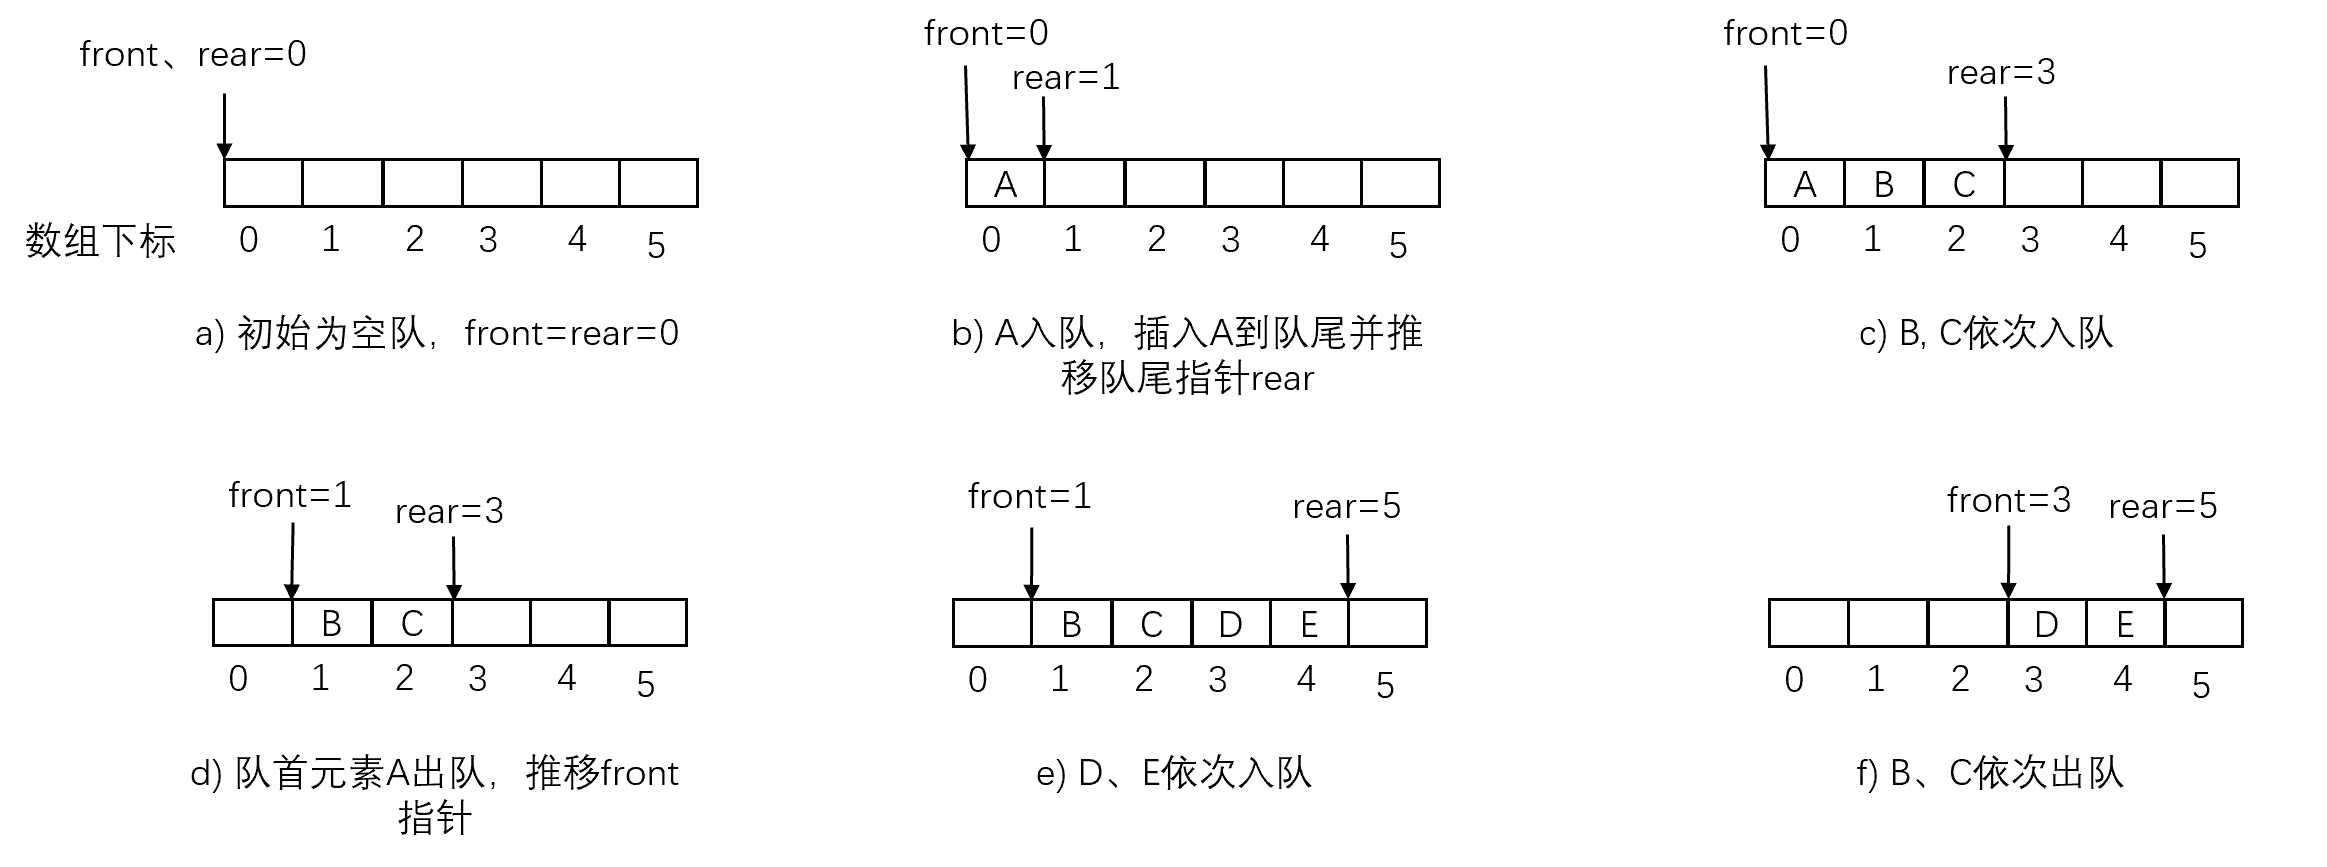
\includegraphics[width=1.05\textwidth]{assets/pics_and_ppts/ch3/在顺序表上实现队列.png}
    \caption{在顺序表上实现队列}
    \label{fig:在顺序表上实现队列}
\end{figure}

然而，一个看似简单的问题很快就会出现：

\begin{quote}
当rear已经走到了数组的尽头，而数组的前半部分却明明还有大量空闲空间时，我们还能继续入队吗？
\end{quote}

例如，一个容量为10的队列，经过几次入队、出队操作后，可能变成：

\[
\underbrace{\square\ \square\ \square\ \square}_{\text{已经出队，空闲}}
\quad
\underbrace{A\ B\ C\ D\ E\ F}_{\text{队列中的元素}}
\]

此时数组中明明还有4个空闲位置，但如果我们把数组看成一条只能从左向右移动的“道路”，rear已经走到了道路的尽头。按照普通顺序表的存储方式，我们似乎只能无奈地宣布：

\[
\text{“队列满了。”}
\]

可是，真的满了吗？

显然不是。相信聪明的你已经想到了，如图\ref{fig:循环队列示意图}所示，当rear走到尽头时，我们可以让rear“回到起点”，继续利用那些已经空闲了的空间，
\term{让rear始终“追着front跑”，当rear真正追上front时，确实没有可利用的空间了，此时才是真正的“队满了”}。
\begin{figure}[htbp]
    \centering
    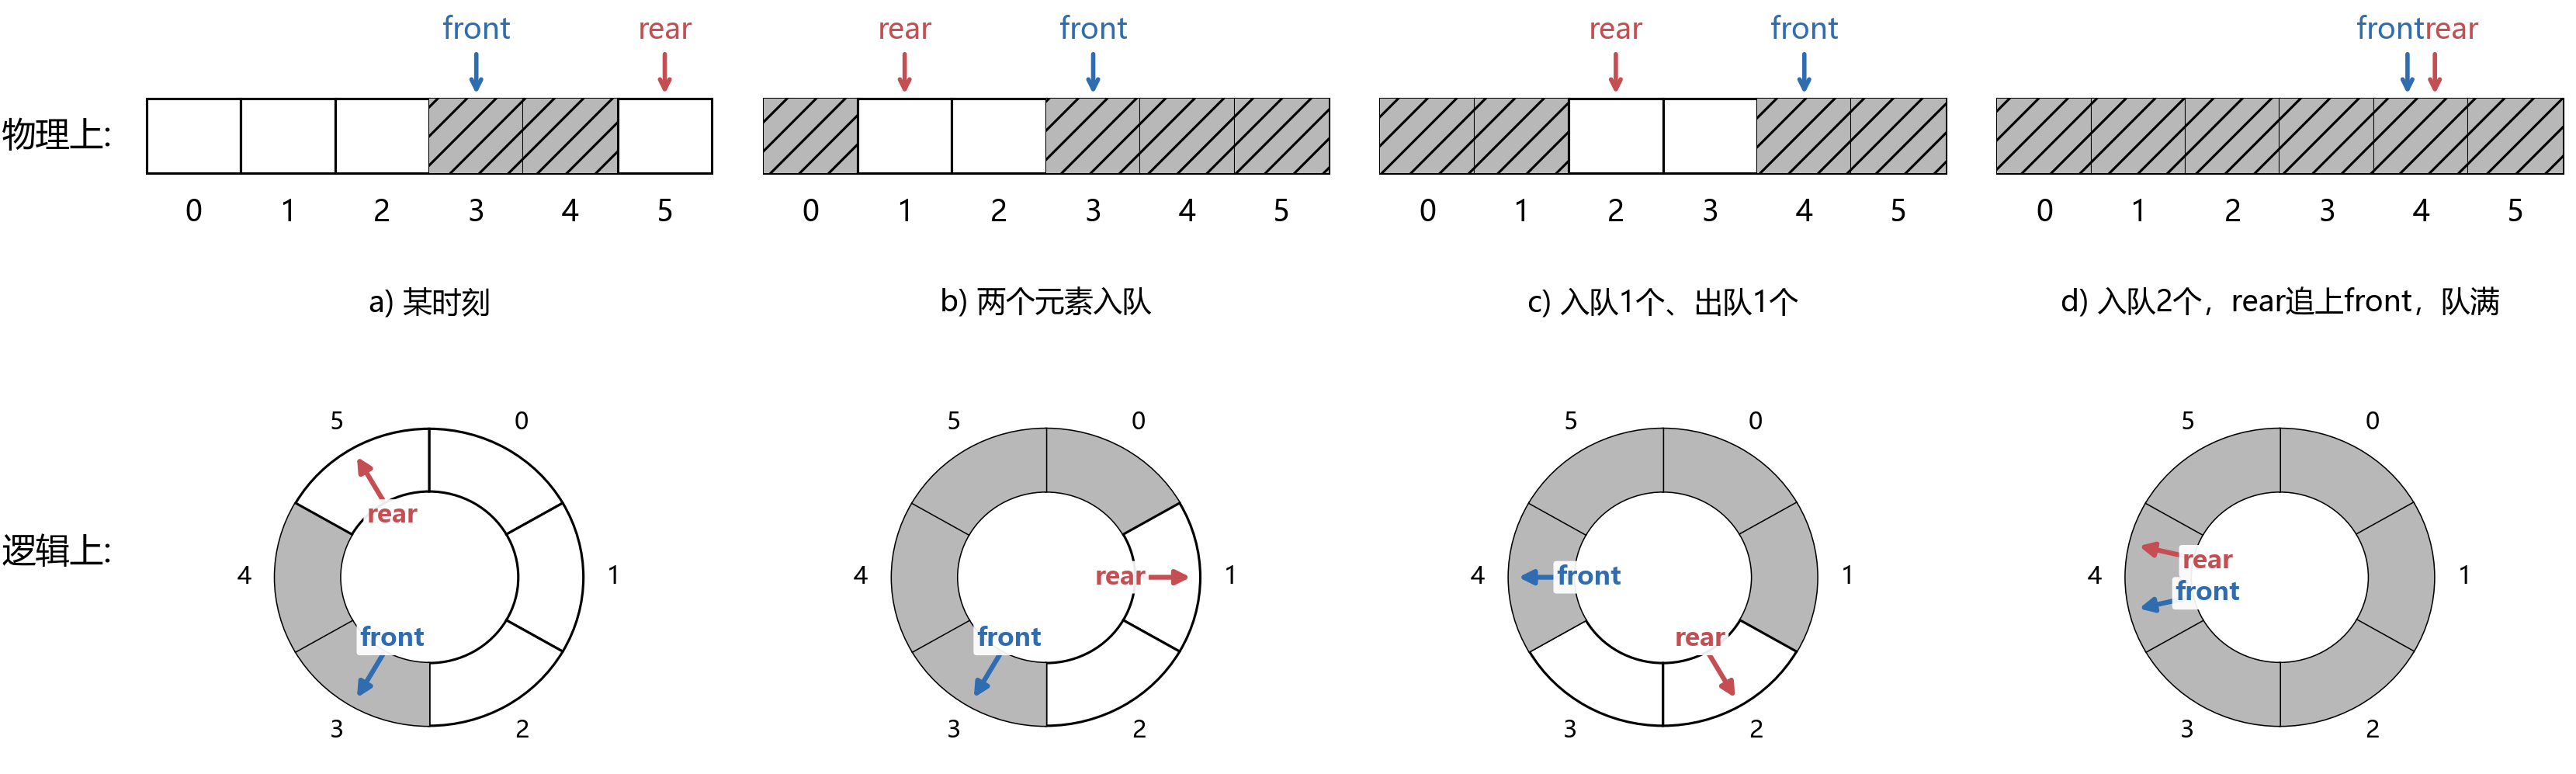
\includegraphics[width=1.10\textwidth]{assets/pics_and_ppts/ch3/循环队列示意图.png}
    \caption{循环队列示意图}
    \label{fig:循环队列示意图}
\end{figure}

这正是\term{循环队列}所要解决的问题。

循环队列不再把数组看成一条有起点、有终点的直线，而是把数组的首尾连接起来：当指针走到数组末尾时，就“绕回”数组开头，整个数组物理上是一条直线，但逻辑上是一个环，
因此叫\term{循环队列}或\term{环形队列}。

\textbf{因此，队列的顺序存储通常都会实现为循环队列}。

“回到起点”，代码上如何实现？举个例子某数组大小为100，下标为0-99，当rear的值已经为99时，如果不加以控制，下一步
将走到100，但我们希望它回到0。不难发现，这正是“取模”运算的功能。因此入队或出队时，若指针从99推移到100，我们将其对100取模，即可重新回到起点0：
\begin{cppcode}
    if(rear > MaxSize-1) {    // 若MaxSize为100，MaxSize-1为最大下标99
        rear = rear % MaxSize;
    }
\end{cppcode}

\begin{insightbox}
    在计算机科学中大家往往喜欢将“取模”和“取余”同等对待，但事实上存在负数参与运算时，取模（modulo）和取余（remainder）数学上的定义可能不同。“\%”运算符事实上更接近
    数学上的取余运算。但这里还是用“取模”来描述，原因在于二者在语感上有差异：“取余”关注的是除法“除完还剩多少”；而“取模”关注的是“映射到哪个模类/固定范围”。
    此处“\%”运算的语义更接近“取模”。
\end{insightbox}

还有第二个问题需要考虑。循环队列如何判断“队空”？可以简单地通过
\begin{bulk}
    \begin{center}
        front == rear \&\& front == 0
    \end{center}
\end{bulk}
来判断吗？经过分析发现是不可以的。因为队满的时候，上面的条件也可能成立。如图\ref{fig:循环队列示意图} ，对于d）所示场景，若再进行两次出队、两次入队，就可以
达成 front == rear \&\& front == 0 的条件，并且此时队列是满的。如何解决这个问题？相信大家自然地想到的做法是多维护一个字段，动态维护队列中当前元素个数：
\begin{cppcodeHighlight}[6]
    #define MaxSize 100
    struct SeqQueue {
        ElemType data[MaxSize];
        int front;
        int rear;
        int current_size;   // 新增字段
    };
\end{cppcodeHighlight}
这当然没问题。但更多教材给出的做法是少利用一个数组空间，通过 (Q.rear+1)\%MaxSize == Q.front 来作为队满的条件，如图\ref{fig:循环队列队满示意图}所示。
\begin{figure}[htbp]
    \centering
    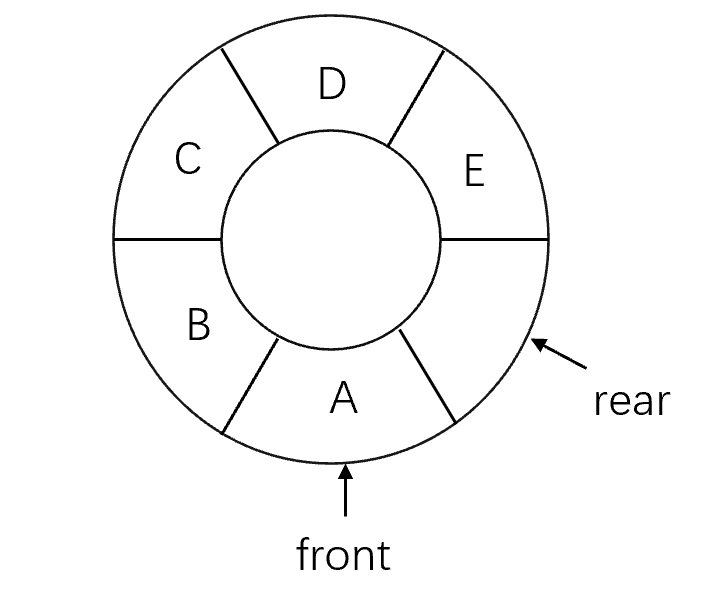
\includegraphics[width=0.28\textwidth]{assets/pics_and_ppts/ch3/循环队列队满示意图.png}
    \caption{队满示意图}
    \label{fig:循环队列队满示意图}
\end{figure}
我们这里遵从多数教材给出的做法，少利用一个数组空间，使用 (Q.rear+1)\%MaxSize == Q.front 来作为队满的条件。同时可以看到，在此做法下，除队空时front和rear初始化
为0之外，其余情况不可能出现 front == rear 的情况（因为我们少利用一个空间，所以rear永远无法追上front，最多只能在它后面一格）。所以可以将 front == rear 直接作为
判断队空的条件。

至此我们已经完成了所有“思维”上的准备，接下来给出循环队列的常见操作实现。

\minisection{1.初始化循环队列}
\begin{cppcode}
    int InitQueue(SeqQueue& q) {
        q.front = q.rear = 0;
        return 1;
    }
\end{cppcode}

\minisection{2.判断队空}
\begin{cppcode}
    int Empty(SeqQueue q) {
        if(q.front == q.rear) {
            return 1;
        }
        return 0;
    }
\end{cppcode}

\minisection{3.入队}
\begin{cppcode}
    int EnQueue(SeqQueue& q, ElemType e) {
        if( (q.rear+1) % MaxSize == q.front) {
            return 0;   // 队满，无法入队
        }

        // 先“放入元素”，再“推移指针”
        q.data[q.rear] = e;
        q.rear += 1;
        if(q.rear>=MaxSize) {
            q.rear = q.rear % MaxSize;
        }
        return 1;
    }
\end{cppcode}

\minisection{4.出队}
\begin{cppcode}
    int DeQueue(SeqQueue& q, ElemType& e) {
        if(Empty(q)) {
            return 0;   // 空队
        }

        // 先“取出元素”，再“推移指针”
        e = q.data[q.front];
        q.front += 1;
        if(q.front >= MaxSize) {
            q.front %= MaxSize;
        }
        return 1;
    }
\end{cppcode}

实际应用中，通常不会有“获取队列中的元素数量”的需求，这里笔者稍作提示：对于循环队列，可以通过下式在O(1)时间得到队列长度：
\begin{bulk}
    \begin{center}
        (rear-front+MaxSize) \% MaxSize
    \end{center}
\end{bulk}
而对于链队列，需要求队列长度，则需要遍历一遍队列（链表），时间复杂度为O(n)。\\

在解决实际问题时，有时会顺其自然地使用到两端均能入队、出队，或一端能入两端能出、两端能入一端能出的队列，它们通常被称为\term{双端队列}。{\color{red}\textbf{相关内容我们通过
习题2作为练习。}}

\section{栈的进一步理解}
提示：本节内容略有难度。\\


栈后进先出的特性，决定了其可以应用于一些很有趣的场景。我们这里先给出一般化的理解：许多场景下，可以用栈来保存这样的数据，即：\textbf{“那些仍然等待未来某个事件发生，并且
优先处理后来者”的数据。}现在看这句话过于抽象，不过别急，本节过后你的心会怦怦直跳。


\bookmark{bookmark:mark-3}{mark-3}
我们给出一例：现在假设天气预报已经报导了未来n天的温度，保存在一个数组temperatures[]中，请你设计一种算法，对于每一天i，找出其后方第一个温度高于第i天的日子。

最直接的办法就是“检查”每一天i，向后扫描，直到找到温度高于i的那一天，之后回到i+1，重复这个过程，伪代码如下所示：
\begin{cppcode}
    for(int i=0; i<n; i++) {
        int found = 0;
        for(int j=i+1; j<n; j++) {
            if(temperatures[j] > temperatures[i]) {
                // 找到了.
                found = 1;
                // j就是要找的那一天

                break;
            }
        }
        if(found == 0) {
            // 第i天的后面没有比第i天温度更高的了。
        }
    }
\end{cppcode}
显然这个算法时间复杂度为O(\(n^2\))。分析以上过程我们会发现，事实上我们做了很多查找是“不必要”的。比如，考虑temperatures[]输入如下：
\begin{bulk}
    \begin{center}
        25, 23, 19, 18, 20, 27, 26, 27
    \end{center}
\end{bulk}
当我们“检查”25时，就由前往后查找到了第一个27的位置，事实上此时我们就已经能够知道23的“答案天”就是27，并且19、18的“答案天”就是20。只不过，此时我们虽然已经
“看到了”这些信息，却没有把它们保存下来。于是，一个很自然的想法出现了：如果我们能通过某种手段将这些\textbf{尚未找到答案的天}记录下来，那么未来的温度出现
时，就可以立即检查这些等待中的天是否能够得到答案。当我们检查25时，将它记下来：
\begin{bulk}
    \begin{center}
        some\_structure: \{25\}
    \end{center}
\end{bulk}
检查23，some\_structure中没有元素会得到答案，将23记下来：
\begin{bulk}
    \begin{center}
        some\_structure: \{25, 23\}
    \end{center}
\end{bulk}
继续检查19、18：
\begin{bulk}
    \begin{center}
        some\_structure: \{25, 23, 19, 18\}
    \end{center}
\end{bulk}
当检查到20时，终于找到了19和18的答案，19和18两个元素期待的事情终于发生，因此将19和18从some\_structure中移出，将20记下来：
\begin{bulk}
    \begin{center}
        some\_structure: \{25, 23, 20\}
    \end{center}
\end{bulk}
你会惊奇地发现一件事情：留存在some\_structure中的温度序列一定是单调不增的，因为低温一定会在高温来到时“找到答案”而被移出。因此当新的温度t来到时，它能移出哪些
温度？其实只需要依次从some\_structure的尾部依次向前比较，“清除”掉some\_structure所有小于t的温度即可，这样一定不会漏。

说到这里你会发现，some\_structure正是满足“只会在一端进行插入删除”。或者换个角度想，当新温度t到来时，后进入some\_structure的元素一定要先被检查，因为后进入
的一定是更小的，如果都不能被t“清理掉”，前面的就更不会被清理掉。

这不就是栈吗！

想通了这一点，这个问题就变得非常简单：我们设一个栈s，保存所有“尚未找到答案”的天，并用一个数组ans[]保存已经得到的答案：ans[i]=j表示i的“答案天”是j。
如图\ref{fig:每日温度}，我们遍历一遍数组，依次检查temperatures[]中
的每一个温度temperatures[j] = t，将其与栈顶温度temperatures[s.top]进行比较，若t大于栈顶温度，则栈顶的这一天s.top的“答案天”就是j，并继续将t与新
的栈顶进行比较，重复这个过程，直至t不大于栈顶温度或栈空后，将当前检查的温度j入栈。检查完所有温度后，栈中剩余的这些天，就是后面没有温度高于他们的。
\begin{figure}[htbp]
    \centering
    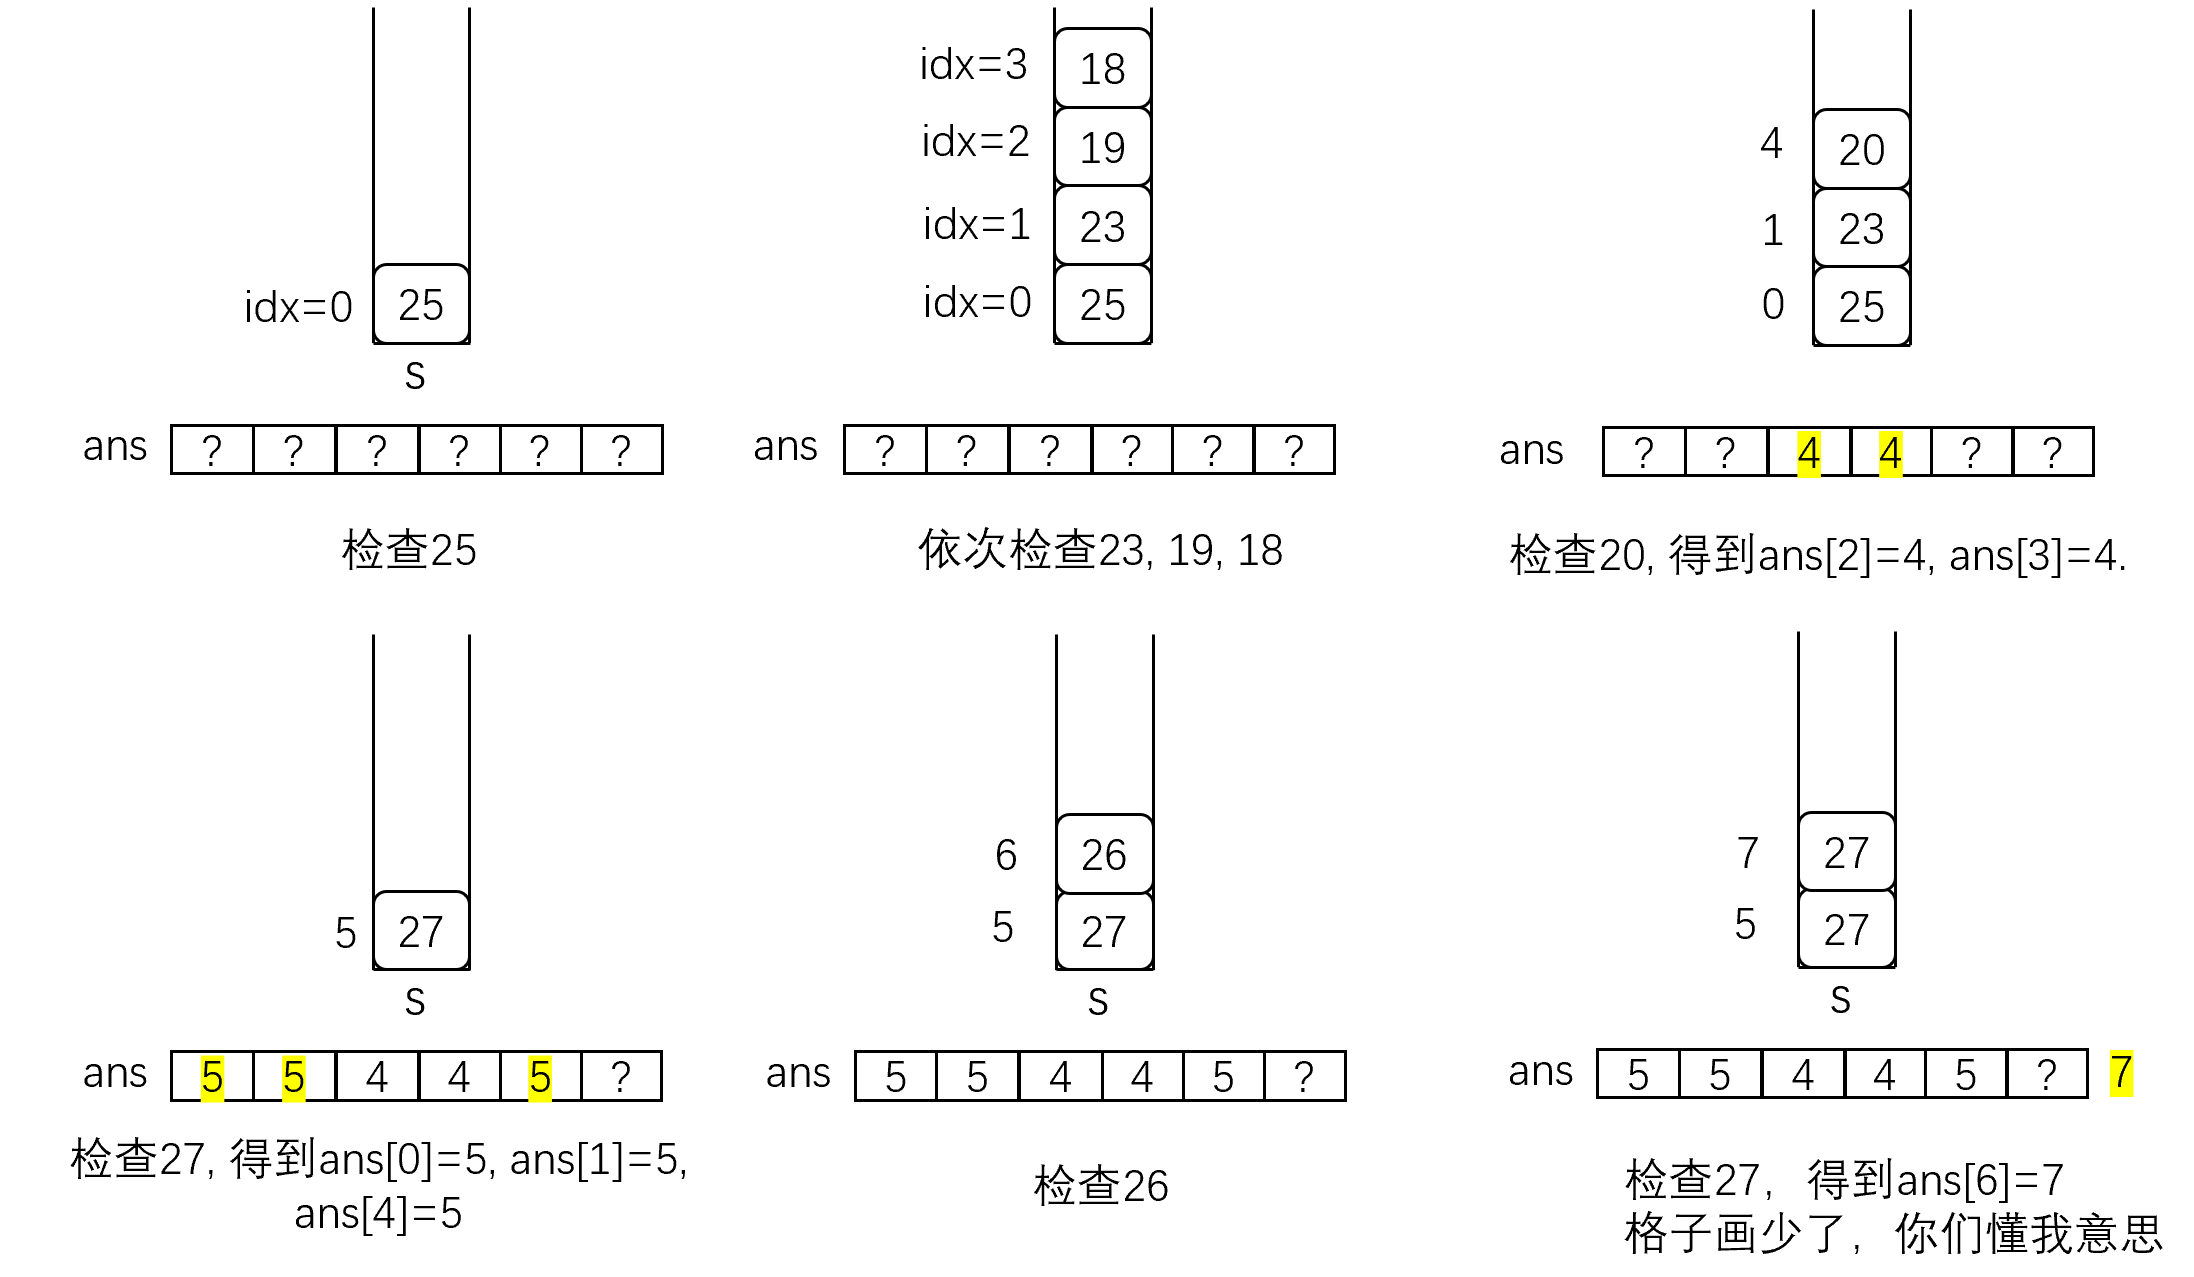
\includegraphics[width=0.81\textwidth]{assets/pics_and_ppts/ch3/每日温度.png}
    \caption{}
    \label{fig:每日温度}
\end{figure}
最后留在栈中的（下标为5和7的）两天，后面没有温度高于它们。伪代码如下所示：
\begin{cppcode}
    for(int i=0; i<n; i++) {
        while(!Empty(s) && temperatures[i]>temperatures[s.top]) {
            ans[s.top] = i;
            Pop(s);
        }
        Push(s, i);
    }
    while(!Empty(s)) {
        ans[s.top] = 0; // 这里拟用0表示后面不存在一天，比s.top这一天温度更高
        Pop(s);
    }
\end{cppcode}

该算法的时间复杂度为O(n)。至于为什么是O(n)，相比于上一种算法，该算法的提升在哪里，这里留给读者自行思考。可以看到，栈s中的元素是单调不增的，很多人喜欢
将这种元素具有单调性的栈称为\term{单调栈}，但笔者希望强调的更多是思考问题、解决问题的这个创造性的过程，次之才是：下次遇见类似的问题，可以用“单调栈”来解决。

相信通过该例大家已经建立了足够的感觉，我们来回看这句话：许多场景下，可以用栈来保存这样的数据，即：\textbf{“那些仍然等待未来某个事件发生，并且
优先处理后来者”的数据。}该例并非巧合，而是存在大量类似的问题，比如大名鼎鼎的\term{“表达式求值”}问题。

\subsection{表达式的转换与求值}
\label{sec:表达式的转换与求值}
表达式的转换与表达式的求值的过程中实际上也有类似上面的思想。
我们先来介绍中缀表达式、后缀表达式的概念。如果你已经了解二者的概念，并且能够熟练地将二者相互转换，请放心地直接跳至\bookmarkref{bookmark:mark-2}{mark-2}处。
我们平时书写算术表达式时，通常采用这样的形式：
\[
3+5
\]
如果表达式稍微复杂一些，例如：
\[
3+5\times2
\]
我们知道应该先计算乘法，再计算加法，这种运算符写在两个操作数之间的表达式，称为\textbf{中缀表达式（Infix Expression）}。

但是，计算机真的喜欢这样的表达式吗？

仔细观察上面的表达式：
\[
3+5\times2
\]
如果我们从左到右依次读取它，会先看到 $3+5$。
可是，此时却不能立即计算，因为后面的乘法具有更高的优先级。
也就是说，当我们看到一个运算符时，
有时可以立即计算，有时却必须\textbf{暂时把它保存起来}，
等待后面的运算符被处理之后才能决定。

如果再加入括号，情况会变得更加复杂：
\[
(3+5)\times2
\]
这时我们不仅需要考虑运算符的优先级，
还需要处理括号所带来的运算顺序。\\

如果我们将
\[
(3+5)\times2
\]
改写成
\[
3\;5\;2\;\times \;+
\]
此时我们再从左向右读取它，你会发现：
\begin{enumerate}
    \item 读取 $3$；
    \item 读取 $5$；
    \item 读取 $2$；
    \item 读取 $\times$，将 $5$ 和 $2$ 相乘，得到10，表达式变成了3 10 +；
    \item 读取 $+$，将 $3$ 和 $10$ 相加，得到最终结果。
\end{enumerate}

整个计算过程不需要我们再判断“乘法是不是应该优先计算”，
因为\textbf{运算符出现的位置本身，就已经把运算顺序表达出来了}。

这种将运算符写在其操作数之后的表达式，称为\textbf{后缀表达式（Postfix Expression）}，也称为\textbf{逆波兰表达式（Reverse Polish Notation，RPN）}。
我们再给出几例。
中缀表达式
\[
b\times c+(a-d)
\]
的后缀形式为：
\[
bc\times ad-+
\]
至于如何手动将中缀转后缀，限于篇幅，此处不再给出，请大家参考CoreLoop本人相关DLC。

中缀表达式
\[
a+b\times c-(b-d)\div e
\]
的后缀形式为：
\[
abc\times +bd-e\div -
\]

在后缀表达式中，每一个运算符都紧跟在它所需要的操作数之后，
因此不需要再使用括号，也不需要额外规定运算符的优先级。

\bookmark{bookmark:mark-2}{mark-2}
\minisection{栈与表达式求值}
我们首先考虑较简单的，计算机如何求值后缀表达式。

计算机按照从左到右的顺序处理后缀表达式，当看到一个数字时，应该把它放在哪里？当看到一个运算符时，又应该从哪里取出它所需要的操作数？

例如，对于：
\[
3\;5\;2\;\times\;+
\]
当读取到 $\times$ 时，需要取出最近读取的两个操作数 $5$ 和 $2$；

而计算出 $5\times2=10$ 后，
又需要把结果暂时保存起来，
等待后面的 $+$。

这种“\textbf{最后保存的操作数最先被取出使用}”的特点，恰好符合栈的\textbf{后进先出}原则。于是，后缀表达式求值的算法就变得很好理解：
对于后缀表达式，我们从左到右依次读取每一个元素：
\begin{itemize}
    \item 如果读取到的是操作数，则将其压入栈中；
    \item 如果读取到的是运算符，则从栈中弹出所需数量的操作数，
          完成运算后，再将运算结果压入栈中。
\end{itemize}
当整个表达式处理完毕后，栈中剩下的唯一元素就是整个表达式的计算结果。

后缀表达式最重要的特点并不是“把运算符放到了后面”，而是：
\begin{quote}
\textbf{它把原本隐藏在括号和运算符优先级中的运算顺序，
直接编码到了表达式的排列顺序中。}
\end{quote}
因此，对于后缀表达式，计算机不再需要理解“谁的优先级更高”，也不需要处理括号的嵌套关系，只需要从左到右读取表达式，并按照遇到的运算符立即进行计算即可。求
后缀表达式
\[
abc\times +bd-e\div -
\]
的值的过程如表\ref{tab:后缀表达式求值过程}所示。

\begin{table}[h]
    \centering
    \caption{后缀表达式求值过程}
    \label{tab:后缀表达式求值过程}

    \renewcommand{\arraystretch}{1.4}

    \begin{tabularx}{\textwidth}{
        >{\centering\arraybackslash}p{0.07\textwidth}
        >{\centering\arraybackslash}p{0.09\textwidth}
        >{\centering\arraybackslash}p{0.12\textwidth}
        >{\raggedright\arraybackslash}X
        >{\centering\arraybackslash}p{0.25\textwidth}
    }

        \toprule
        步骤
        & 扫描项
        & 项类型
        & 动作
        & 栈中内容（栈底 $\rightarrow$ 栈顶）
        \\
        \midrule

        1
        & $a$
        & 操作数
        & $a$ 入栈
        & $a$
        \\

        2
        & $b$
        & 操作数
        & $b$ 入栈
        & $a,\ b$
        \\

        3
        & $c$
        & 操作数
        & $c$ 入栈
        & $a,\ b,\ c$
        \\

        4
        & $\times$
        & 运算符
        & 弹出 $b$、$c$，计算 $b\times c$，
          将结果 $bc$ 入栈
        & $a,\ bc$
        \\

        5
        & $+$
        & 运算符
        & 弹出 $a$、$bc$，计算 $a+bc$，
          将结果入栈
        & $a+bc$
        \\

        6
        & $b$
        & 操作数
        & $b$ 入栈
        & $a+bc,\ b$
        \\

        7
        & $d$
        & 操作数
        & $d$ 入栈
        & $a+bc,\ b,\ d$
        \\

        8
        & $-$
        & 运算符
        & 弹出 $b$、$d$，计算 $b-d$，
          将结果入栈
        & $a+bc,\ b-d$
        \\

        9
        & $e$
        & 操作数
        & $e$ 入栈
        & $a+bc,\ b-d,\ e$
        \\

        10
        & $\div$
        & 运算符
        & 弹出 $b-d$、$e$，计算
          $\dfrac{b-d}{e}$，将结果入栈
        & $\displaystyle a+bc,\ \frac{b-d}{e}$
        \\

        11
        & $-$
        & 运算符
        & 弹出 $a+bc$、$\dfrac{b-d}{e}$，
          计算 $\displaystyle a+bc-\frac{b-d}{e}$，
          将结果入栈
        & $\displaystyle a+bc-\frac{b-d}{e}$
        \\

        \bottomrule

    \end{tabularx}
\end{table}


事实上，计算机可以\textbf{直接求值中缀表达式}，而无需先将中缀表达式转换为后缀表达式，再进行求值。接下来我们来看计算机如何直接求值中缀表达式。
与后缀表达式不同的是，当计算机从左到右读取中缀表达式时，遇到一个运算符op后，不能总是立即计算。某些运算符必须暂时保存下来，等待后面的运算符出现之后，
才能决定自己什么时候参与计算。有了前面的思想很容易知道，扫描过程中遇到的运算符op就是\textbf{“那些仍然等待未来某个事件发生，并且优先处理后来者”}的数据。

于是，一个非常自然的设计出现了：

\begin{itemize}
    \item \textbf{操作数栈：}保存当前暂时不能参与运算的操作数以及中间计算结果；
    \item \textbf{运算符栈：}保存当前暂时不能执行的运算符。
\end{itemize}

当计算机从左到右读取一个中缀表达式时，可以按照下面的规则进行处理：

\begin{enumerate}
    \item 从左到右依次读取中缀表达式中的每一个元素。
    \item 如果读取到的是操作数，则将其压入操作数栈。
    \item 如果读取到的是左括号，则将其压入运算符栈。
    \item 如果读取到的是右括号，则不断弹出运算符栈的栈顶运算符，
    从操作数栈中取出相应的操作数进行计算，并将计算结果重新压入操作数栈，
    直到遇到左括号为止。最后将左括号弹出并丢弃。
    \item 如果读取到的是运算符，则比较当前运算符与运算符栈栈顶运算符的优先级：
    \begin{itemize}
        \item 如果运算符栈为空，或者栈顶为左括号，或者当前运算符的优先级高于栈顶运算符，
        则将当前运算符压入运算符栈；
        \item 否则，不断弹出栈顶运算符，从操作数栈中取出相应的操作数进行计算，
        并将计算结果重新压入操作数栈，直到当前运算符可以入栈为止，
        然后将当前运算符压入运算符栈。
    \end{itemize}
    \item 中缀表达式读取完毕后，不断弹出运算符栈中的运算符，
    从操作数栈中取出相应的操作数进行计算，并将计算结果重新压入操作数栈。
    \item 当运算符栈为空时，操作数栈中剩余的唯一元素即为整个中缀表达式的计算结果。
\end{enumerate}

这样，我们就不需要先将中缀表达式转换成后缀表达式，而是可以直接在读取中缀表达式的过程中完成计算。

这个过程我没有画图，并不是因为懒，而是相信通过前面的寻找温度的例子，你已经对类似场景建立了足够的直觉。如果你还没有搞清楚“栈与表达式”是怎么回事，
可以参考CoreLoop本书相关的DLC。


\minisection{*栈与表达式转换}
根据前面的介绍，事实上计算机可以借助两个栈，直接计算中缀表达式的值。但出于某种原因，这里我们依然介绍一下计算机如何借助栈将中缀表达式转换为后缀表达式。
有了前面的内容相信大家已经能够自行想出正确的做法了。我们这里直接给出：
\begin{enumerate}
    \item 从左到右依次读取中缀表达式中的每一个元素。
    \item 如果读取到的是操作数，则直接将其加入后缀表达式。
    \item 如果读取到的是左括号，则将其压入运算符栈。
    \item 如果读取到的是右括号，则不断弹出运算符栈的栈顶元素，
    并将其加入后缀表达式，直到遇到左括号为止。
    左括号弹出后丢弃，不加入后缀表达式。
    \item 如果读取到的是运算符，则比较它与运算符栈栈顶运算符的优先级：
    \begin{itemize}
        \item 如果栈为空，或者栈顶为左括号，或者当前运算符的优先级高于栈顶运算符，
        则将当前运算符压入栈中；
        \item 否则，不断弹出栈顶运算符并加入后缀表达式，
        直到当前运算符可以入栈为止。
    \end{itemize}
    \item 中缀表达式读取完毕后，将运算符栈中剩余的运算符依次弹出，
    并加入后缀表达式。
\end{enumerate}
整个过程的核心其实非常简单：
\begin{quote}
\textbf{操作数直接输出，运算符暂存于栈中；当一个运算符已经可以确定其位置时，
就将它从栈中弹出并输出。}
\end{quote}
中缀表达式
\[
a+b\times c-(b-d)\div e
\]
转后缀表达式的过程如表\ref{tab:中缀转后缀过程}所示。
\begin{table}[htbp]
    \centering
    \caption{中缀表达式转换为后缀表达式的过程}
    \label{tab:中缀转后缀过程}

    \renewcommand{\arraystretch}{1.35}

    \begin{tabularx}{\textwidth}{
        >{\centering\arraybackslash}p{0.06\textwidth}
        >{\centering\arraybackslash}p{0.09\textwidth}
        >{\centering\arraybackslash}p{0.12\textwidth}
        >{\raggedright\arraybackslash}X
        >{\centering\arraybackslash}p{0.20\textwidth}
        >{\centering\arraybackslash}p{0.20\textwidth}
    }

        \toprule
        步骤
        & 扫描项
        & 项类型
        & 动作
        & 运算符栈（栈底 $\rightarrow$ 栈顶）
        & 后缀表达式
        \\
        \midrule

        1
        & $a$
        & 操作数
        & $a$ 直接输出
        &
        &
        $a$
        \\

        2
        & $+$
        & 运算符
        & 栈为空，$+$ 入栈
        &
        $+$
        &
        $a$
        \\

        3
        & $b$
        & 操作数
        & $b$ 直接输出
        &
        $+$
        &
        $ab$
        \\

        4
        & $\times$
        & 运算符
        & $\times$ 的优先级高于栈顶的 $+$，
          $\times$ 入栈
        &
        $+,\ \times$
        &
        $ab$
        \\

        5
        & $c$
        & 操作数
        & $c$ 直接输出
        &
        $+,\ \times$
        &
        $abc$
        \\

        6
        & $-$
        & 运算符
        & $-$ 的优先级低于栈顶的 $\times$，
          弹出 $\times$ 并输出；
          $-$ 的优先级与栈顶的 $+$ 相同，
          弹出 $+$ 并输出；然后 $-$ 入栈
        &
        $-$
        &
        $abc\times+$
        \\

        7
        & $($
        & 左括号
        & 左括号直接入栈
        &
        $-,\ ($
        &
        $abc\times+$
        \\

        8
        & $b$
        & 操作数
        & $b$ 直接输出
        &
        $-,\ ($
        &
        $abc\times+b$
        \\

        9
        & $-$
        & 运算符
        & 栈顶为左括号，不进行优先级比较，
          $-$ 直接入栈
        &
        $-,\ (,\ -$
        &
        $abc\times+b$
        \\

        10
        & $d$
        & 操作数
        & $d$ 直接输出
        &
        $-,\ (,\ -$
        &
        $abc\times+bd$
        \\

        11
        & $)$
        & 右括号
        & 依次弹出栈顶运算符并输出；
          遇到左括号后将其弹出，但不输出
        &
        $-$
        &
        $abc\times+bd-$
        \\

        12
        & $\div$
        & 运算符
        & $\div$ 的优先级高于栈顶的 $-$，
          $\div$ 入栈
        &
        $-,\ \div$
        &
        $abc\times+bd-$
        \\

        13
        & $e$
        & 操作数
        & $e$ 直接输出
        &
        $-,\ \div$
        &
        $abc\times+bd-e$
        \\

        14
        & 结束
        & —
        & 扫描结束，将栈中剩余的运算符依次弹出并输出
        &
        —
        &
        $abc\times+bd-e\div-$
        \\

        \bottomrule

    \end{tabularx}
\end{table}


\clearpage%%%%%%%%%%%%%%%%%%%%%%%%%%%%%%%%%%%%%%%%%%%%%%%%%%%%%%%%%%%%%%%%%%%%%%%%%%%%%%%%%%%%%%%%%%%%%%%%%%%%%%%%%%%%%%%%%%%%%%%%%%%%%%%%%%%%%%%%%%
\begin{exercise}
    1. [多选]下列说法正确的是$\underline{\hspace{1cm}}$。\\
A. 栈是一种有特殊要求的线性表。\\
B. 队列是一种有特殊要求的线性表。\\
C. 最先入栈的元素一定最先出栈。\\
D. 最先入队的元素一定最先出队。\\

    2. 以下哪一项不是栈可以进行的操作？$\underline{\hspace{1cm}}$\\
A. 将元素压入栈中\\
B. 判断栈是否为空\\
C. 删除栈底元素\\
D. 将栈置为空栈\\

    3. 以下哪一项不是队列可以进行的操作？$\underline{\hspace{1cm}}$\\
A. 将元素插入队尾\\
B. 获取队首元素的值\\
C. 获取位序为i的元素的值\\
D. 位序为i的元素出队\\

    4. 某个栈，元素的入栈序列是 $$ 1,2,3,4 $$ 则以下序列中，不可能作为出栈序列的是：$\underline{\hspace{1cm}}$\\
A. 2, 1, 3, 4\\
B. 2, 3, 4, 1\\
C. 3, 2, 4, 1\\
D. 3, 4, 1, 2\\

    5. 关于时间复杂度，以下说法正确的是：\\
A. 顺序栈的 Push 和 Pop 时间均为 \(O(n)\)\\
B. 链栈的 Push 和 Pop 均可实现为 \(O(1)\)\\
C. 使用单链表实现队列时，只要有 head 指针，入队和出队均可实现为 \(O(1)\)\\
D. 循环队列的入队操作必须移动大量元素，因此时间复杂度为 O(n)\\

    6. 采用数组实现容量为 \(N\) 的循环队列，并规定：\\
front 指向队首元素；\\
rear 指向下一个插入位置；\\
front和rear初始全部指向下标\(N-1\)处，队列采用保留一个空闲位置的方式区分队满和队空。

则判断队列为空和队满的条件分别为：\\
A. front == 0 \&\& rear == 0, rear + 1 == front\\
B. front == 0 \&\& rear == 0, (rear + 1) \% N == front\\
C. front == rear, rear + 1 == front\\
D. front == rear, (rear + 1) \% N == front \\

    7. [多选]某同学做了如下设计：采用一个长度为100的数组实现两个栈S1和S2。该同学规定两栈栈底分别在两个端点处，栈顶向中间生长，如图\ref{fig:共享栈}。
    同时规定两栈栈顶元素相邻时，存储空间满，均无法再入栈。
\begin{figure}[htbp]
    \centering
    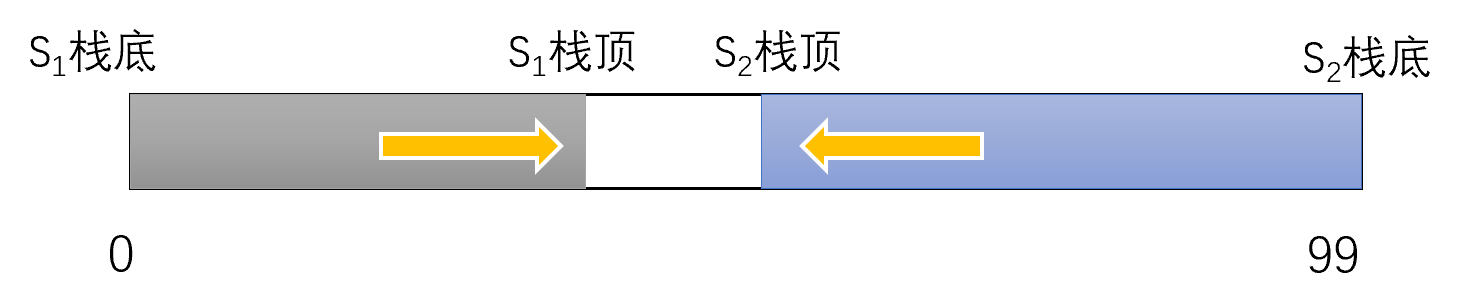
\includegraphics[width=0.67\textwidth]{assets/pics_and_ppts/ch3/共享栈.png}
    \caption{}
    \label{fig:共享栈}
\end{figure}
    以下说法中正确的是$\underline{\hspace{1cm}}$\\\\
\textbf{A.} 两栈入栈时间复杂度均为O(1)\\
\textbf{B.} 设两栈元素数量分别为n、m，则两栈栈顶元素的出栈时间复杂度分别为O(n)、O(m)\\
\textbf{C.} 要计算两栈栈中已有元素数量之和，时间复杂度为O(1)\\\\
\textbf{D.} 若S1.top初始化为-1，S2.top初始化为100，且两个栈顶指针始终指向各自的栈顶元素，则S1.top+1==S2.top时，空间满，两栈均无法再入栈\\
\textbf{E.} 若S1.top初始化为-1，S2.top初始化为100，且两个栈顶指针始终指向各自的栈顶元素，则可能出现S1.top>S2.top\\
\textbf{F.} 若S1.top初始化为0，S2.top初始化为99，且两个栈顶指针始终指向各自栈顶元素的下一个位置，则S1.top+1==S2.top时，空间满，两栈均无法再入栈\\
\textbf{G.} 若S1.top初始化为0，S2.top初始化为99，且两个栈顶指针始终指向各自栈顶元素的下一个位置，则可能出现S1.top>S2.top\\


    8. 一个初始为空的栈和一个初始为空的队列，都依次接收：
$$ 1,2,3,4,5 $$
如果只允许进行正常的入栈、出栈、入队、出队操作，关于它们能够产生的输出顺序，下列说法正确的是：\\
A. 栈和队列都可以产生任意排列\\
B. 栈只能产生一种输出顺序，队列也只能产生一种输出顺序\\
C. 队列的输出顺序固定为 \(1,2,3,4,5\)，而栈的输出顺序受到栈操作过程限制\\
D. 栈的输出顺序固定为 \(5,4,3,2,1\)，队列的输出顺序受到操作过程限制\\
    
    9.[多选]假设输入序列是1,2,3,4,5，利用两个队列进行出入队操作，不可能的输出序列有$\underline{\hspace{1cm}}$\\
A. 5,4,3,2,1\\
B. 5,1,2,3,4\\
C. 5,2,3,1,4\\
D. 2,3,4,5,1\\

    10. [多选]与循环队列相比，链式队列$\underline{\hspace{1cm}}$\\
A. 优点是进队和出队时间复杂度更低\\
B. 优点是长度可以在内存限制内动态变化\\
C. 缺点是节点除数据外需要额外的存储空间存放指针\\
D. 缺点是不能根据队首和队尾指针以O(1)时间算出队列长度\\

    11. 假设某队列采用带头结点的循环双链表实现，第一个数据节点表示队头，最后一个数据节点表示队尾。若只设头指针指向头节点，则进队和出队的时间复杂度分别为：\\
A. O(1), O(1) \\
B. O(1), O(n)\\
C. O(n), O(1)\\
D. O(n), O(n)\\

    12. （某年408真题）现有队列Q和栈S，初始时Q中的元素依次是1,2,3,4,5,6（1在队头），S为空。若仅允许下列的3种操作：\Circled{1}出队并输出出队元素；\Circled{2}出队
    并将出队元素入栈；\Circled{3}出栈并输出出栈元素。则不能得到的输出序列是$\underline{\hspace{1cm}}$\\
A. 1,2,5,6,4,3\\
B. 2,3,4,5,6,1\\
C. 3,4,5,6,1,2\\
D. 6,5,4,3,2,1\\

    13. （某年408真题）某队列允许在其两端进行入队操作，但仅允许在一端进行出队操作。若元素a,b,c,d,e依次入此队列后再进行出队操作，则不可能得到的出队序列是$\underline{\hspace{1cm}}$\\
A. b,a,c,d,e\\
B. d,b,a,c,e\\
C. d,b,c,a,e\\
D. e,c,b,a,d\\

    14. （某年408真题）初始为空的队列Q的一端仅能进行入队操作，另外一端既能进行入队操作，又能进行出队操作。若Q的入队序列是1,2,3,4,5，则不能得到的出队序列是$\underline{\hspace{1cm}}$\\
A. 5,4,3,1,2\\
B. 5,3,1,2,4\\
C. 4,2,1,3,5\\
D. 4,1,3,2,5\\

    15. （某年408真题）假设栈初始为空，将中缀表达式a/b+(c*d-e*f)/g转换为等价的后缀表达式的过程中，当扫描到f时，栈中的元素依次是$\underline{\hspace{1cm}}$\\
A. +(*-\\
B. +(-*\\
C. /+(*-*\\
D. /+-*\\

    16. （某年408真题）若栈S1中保存整数，栈S2中保存运算符，函数F()依次执行下述的各步操作：\\
    1) 从S1中依次弹出两个操作数a和b；\\
    2) 从S2中弹出一个运算符op；\\
    3) 执行相应的运算b op a；\\
    4) 将运算结果压入S1中。\\
    假定S1中的操作数依次是5,8,3,2（2在栈顶），S2中的运算符依次是*, -, +（+在栈顶）。调用3次F()后，S1栈顶保存的值是$\underline{\hspace{1cm}}$\\
    A. -15\\
    B. 15\\
    C. -20\\
    D. 20\\

    *17. 某游戏服务器持续记录某位名为CoreLoop的玩家的网络延迟情况。现假设服务器连续记录了 \(n\) 个时刻的网络延迟，第 \(i\) 个时刻的延迟为 delay[i]，
    这些数值均为正整数。为防止数值闪动，该服务器将时刻i的近k个时刻延迟的最大值作为该玩家在时刻i的\textbf{显示延迟}。
    也就是说，时刻i的显示延迟为：
    \[
        max(delay[max(0, i-k+1)], delay[max(0, i-k+2)], ..., delay[i])
    \]

    如，对于：
    \[
        delay[] = {40, 33, 38, 37, 42, 35}
    \]

    k=3时，显示延迟为
    \[
        ans[]   = {40, 40, 40, 38, 42, 42}
    \]

    k=4时，显示延迟为
    \[
        ans[]   = {40, 40, 40, 40, 42, 42}
    \]
    请你设计一个尽可能高效的算法，求出该玩家这n个时刻的\textbf{显示延迟}。
    \begin{cppcode}
    // 将时刻0到n-1的显示延迟保存在ans[]数组下标0到n-1处。
        void MaxDelay(int delay[], int n, int k, int ans[]) {

        }
    \end{cppcode}



\end{exercise}
\clearpage

\begin{exerciseanswer}
    1. 选ABD。\\

    2. 选C。栈的插入删除只能在栈顶进行，C错误。\\

    3. 选D。对于C项，队列仅要求队首元素可以出队，但没要求仅队首元素可以被读取。你当然可以为队列实现获取第i个元素的函数接口，但通常来说我们使用队列的场景往往不会有这个需求。
    额外提示：你当然可以为你的“队列”实现第i个元素“出队”的函数接口，但这样做的话，你所实现的数据结构就不能叫做\term{队列}了。\\

    4. 选D。2134可由入入出出入出入出达成；2341可由入入出入出入出出达成；3241可由入入入出出入出出达成；栈满足后进先出，如论如何4一定比3先出，2一定比1先出，D无法达成。\\

    5. 选B。对于A，顺序栈的Push和Pop操作均在顺序表的表尾实现，时间均可达到O(1)；对于C，仅有head指针的单链表实现“头删”，即出队，可达到O(1)，但要实现“尾删”，即出队，
    则需要先找到最后一个节点，时间为O(n)。单链表中额外记录一个尾指针rear，则入队和出队均可达成O(1)时间。对于D，循环队列的入队和出队无需移动元素。\\

    6. 选D。通过本题给了我们一个提示，对于循环队列来说，初始front和rear不一定非要指向0，因为从环的几何结构来讲，“队首元素”保存在0位置和保存在i位置是没有区别的。
    仅有初始状态（队空）会满足front == rear。\\

    7. 选A、C、D、G。对于B，无论栈中有多少个元素，一次出栈操作只需要访问当前栈顶元素，然后修改栈顶指针即可，时间复杂度为O(1)。\\
    对于C，可由两栈的栈顶下标直接分别计算得到两栈的元素数量，时间均为O(1)，再相加即可得到总数量，总体时间为O(1)，C正确；\\
    对于D，要注意：当栈S2中没有元素，而栈S1将空间全部占满时，同样可以用S1.top+1==S2.top判断空间满，当S2将空间占满时同样如此，D正确；\\
    E、F显然错误；\\
    对于G，当栈满时，S1.top指向S1栈顶元素的下一个位置，即S2的栈顶元素位置；对应地，S2.top指向S1的栈顶元素位置，S1.top>S2.top成立，G正确。\\

    8. 选C。队列的特性决定了第i个入队的元素一定是第i个出队的，而栈则不同，栈的出栈顺序是会受到操作过程影响的，{\color{red}\textbf{参考本习题第4题}}。\\

    9. 选AC。\\

    10. 选BCD。\\

    11. 选A。对于循环双链表，可以在O(1)时间立即拿到尾节点指针，因此在头、尾操作均为O(1)。\\

    12. 选C。A项可以通过\Circled{1}\Circled{1}\Circled{2}\Circled{2}\Circled{1}\Circled{1}\Circled{3}\Circled{3}得到；
    B项可通过\Circled{2}\Circled{1}\Circled{1}\Circled{1}\Circled{1}\Circled{1}\Circled{3}得到；
    D项输入与输出刚好相反，显然通过栈就能逆序：\Circled{2}\Circled{2}\Circled{2}\Circled{2}\Circled{2}\Circled{2}\Circled{3}\Circled{3}\Circled{3}\Circled{3}\Circled{3}\Circled{3}。
    对于C，3在1、2前输出，因此1、2必按顺序先入栈，所以1必晚于2输出，C错误。\\

    13. 选C。这是一个非常有意思的题。不妨假设仅有左边能出队。无论如何a一定先入队，摆在最中央的位置。接下来，每一个元素入队，你都可以选择将其“摆在队中已有元素的左边或右边”。所以你需要
    以a为中心努力地去构造四个选项所给出的序列。如A选项要求的序列是b,a,c,d,e，于是你将b摆在a左边，将c摆在ba的右边，将d摆在bac的右边，再将e摆在bacd的右边，便得到
    了A项所要求的序列，从左边出队，便得到了b,a,c,d,e。B、D项也都可以通过同样的方法得到。\\

    14. 选D。\\
    
    15. 选B。详细过程已经在\ref{sec:表达式的转换与求值}中介绍过，不再赘述。\\

    16. 选B。本题比较简单，注意出栈顺序别搞错，同时注意二元运算符op的操作数顺序是b op a而不是a op b，不要搞错就行。\\

    17. 这个问题如果你在思考的过程中自然地想到了使用某种“一端进，两端出”的数据结构，那么你可以开一瓶香槟庆祝一下。如果你只想到了时间复杂度为\(O(n\times k)\)的算法，
    你应该惩罚自己周末不许出去玩。

    本题最容易想到的方法是：从前向后遍历一遍delay[]数组，检查每一个延迟数值delay[i]时，从i向前找，直到遇见下标0或i-k+1的元素，在这个过程中记录下一个最大值，作为
    i时刻的延迟最大值，即ans[i]。该方法的时间复杂度为\(O(n\times k)\)。当k较大时，复杂度可能接近\(O(n^2)\)。\\

    但是，以上方法与“天气预报问题”（见\bookmarkref{bookmark:mark-3}{mark-3}处）的朴素解法有着类似的问题：当我们检查后面的元素时，前面的元素其实已经被检查过若干
    遍了。我们能不能在每个元素第一次被检查的时候，就想办法将它保存到某个结构some\_structure中，直至该元素“不可能成为后面任何一个i的解”，再将它丢弃呢？\\

    我们从前向后遍历，当检查下标为i的元素时：\\
    1）显然，下标<=i-k的元素已经不再可能成为后面任何一个元素（包括i）的解。所以需要将所有下标<=i-k的元素移出some\_structure。这正是“先进先出”。\\
    2）当我们检查i时，由于i可以作为自己的解，所以some\_structure中所有值小于i的元素均已不再可能成为后面任何一个元素的解，移出它们。经过分析不难发现，
    该特性决定了some\_structure中元素单调不增。所以移出时应该将delay[i]与“后进来的”元素先比较。

    所以这个结构应该是一个“尾端能进能出、首端能出”的一个结构。并且当检查元素i时，移出满足上述1）、2）条件的元素后，队首元素就是该元素i的解。
    
    如正文中介绍过，通常称其为\term{双端队列}。此处我们是在解决问题（而不是封装某种数据结构给别人或自己复用），因此
    我们不兴师动众地封装一个“双端队列”的数据结构，并为他写出“首端出队”、“尾端入队、尾端出队”等操作，而是直接将操作展开，作为逻辑的一部分实现。完整代码如下所示。
    \begin{cppcode}
        void MaxDelay(int delay[], int n, int k, int ans[]) {
            // deque[] 保存候选元素的下标。
            // deque[front] 是队首，deque[rear - 1] 是队尾。
            int deque[n];
            int front = 0;
            int rear = 0;

            for (int i = 0; i < n; i++) {
                while (front < rear && deque[front] <= i - k) {
                    // 动态维护队首元素（i的解）
                    front++;     // 注意入队元素一定不会超过n，因此不用考虑循环
                }

                // 移除所有不可能再成为最大值的元素。
                while (front < rear &&
                    delay[deque[rear - 1]] <= delay[i]) {
                    rear--;
                }

                // 当前元素加入队尾。
                deque[rear] = i;
                rear++;

                // 队首就是当前窗口中的最大值。
                ans[i] = delay[deque[front]];
            }
        }
    \end{cppcode}
    

\end{exerciseanswer}
\chapter{树与二叉树}
\section{树}
在\ref{sec:数据结构}节中，我们已经对“什么是树”有了一个感性的认知。与现实中的大树类似，数据结构中的树也是一种由根开始分叉生长的结构。
比如游戏中一个队长三个队员的四人小队可以看成一棵树：
\begin{bulk}
\begin{center}
\begin{tikzpicture}
[
    level distance=1.2cm,
    sibling distance=2cm
]
\node[treenode]{邪念}
    child {
        node[treenode]{银心}
    }
    child {
        node[treenode]{甘尔}
    }
    child {
        node[treenode]{张三}
    };
\end{tikzpicture}
\end{center}
\end{bulk}

你的个人计算机中目录结构的组织是一棵树：
\begin{bulk}
\begin{center}
\begin{tikzpicture}
[
    level distance=1.2cm,
    level 1/.style={
        sibling distance=6cm
    },
    level 2/.style={
        sibling distance=1.8cm
    },
    level 3/.style={
        sibling distance=1.5cm
    },
]
\node[treenode]{此电脑}
    child {
        node[treenode]{本地磁盘(C:)}
        child{
            node[treenode]{Program Files}
        }
        child{
            node[treenode]{Windows}
        }
        child{
            node[treenode]{用户}
        }
        child {
            node[treenode]{...}
        }
    }
    child {
        node[treenode]{新加卷(D:)}
        child{
            node[treenode]{电影}
            child {
                node[treenode]{泰坦尼克号}
            }
            child {
                node[treenode]{...}
            }
        }
        child{
            node[treenode]{照片}
        }
        child {
            node[treenode]{...}
        }
    };
\end{tikzpicture}
\end{center}
\end{bulk}

下面给出树的定义。
\begin{definitionbox}

    \term{树}是$n$（n>=0）个数据元素组成的有限集合，当n=0时，称为\term{空树}。任何一棵非空树都满足以下条件：
    
    \begin{enumerate}
        \item 有且仅有一个数据元素无前驱，称为\term{根节点}；
        \item 除根节点外，其余每个数据元素都有且仅有一个前驱节点，称为\term{父节点}；
        \item 每个数据元素可以有零个或多个后继节点，称为\term{子节点}。
    \end{enumerate}

\end{definitionbox}

由以上定义可知，对于一棵非空树中的任意一个节点，以该节点为根节点，连同该节点的所有后代节点在内所构成的仍是一棵树，称为原树的一棵\term{子树}。
通常认为一棵树本身是自己的子树。很少存在一些场景会关心树中节点的各个子树从左至右是否有次序（即互换后还能不能认为是同一棵树），但通常将节点有次序的树称为
\term{有序树}，节点没有次序的树称为\term{无序树}。

“树”这个逻辑结构该如何实现？如果采用链表类似的思想，每个节点除保存数据外，再保存所有指向其孩子节点的指针，像这样：
\begin{cppcode}
    struct TreeNode {
        ElemType data;
        TreeNode* child1;
        TreeNode* child2;
        TreeNode* child3;
        ...
    }
\end{cppcode}
显然，我们无法预知每个节点有多少孩子节点，因此无法为TreeNode结构定义固定数量的孩子节点指针。
熟悉C++的同学可能会想到，可以使用一个不定长数组，将节点的所有孩子指针保存到该数组中：
\begin{cppcode}
    struct TreeNode {
        ElemType data;
        std::vector<TreeNode*> childs;  // childs是一个不定长数组，childs[0], ..., childs[n]分别表示该节点的各个孩子节点指针
    }
\end{cppcode}
如图\ref{fig:用不定长数组表示树的孩子}所示。
\begin{figure}[htbp]
    \centering
    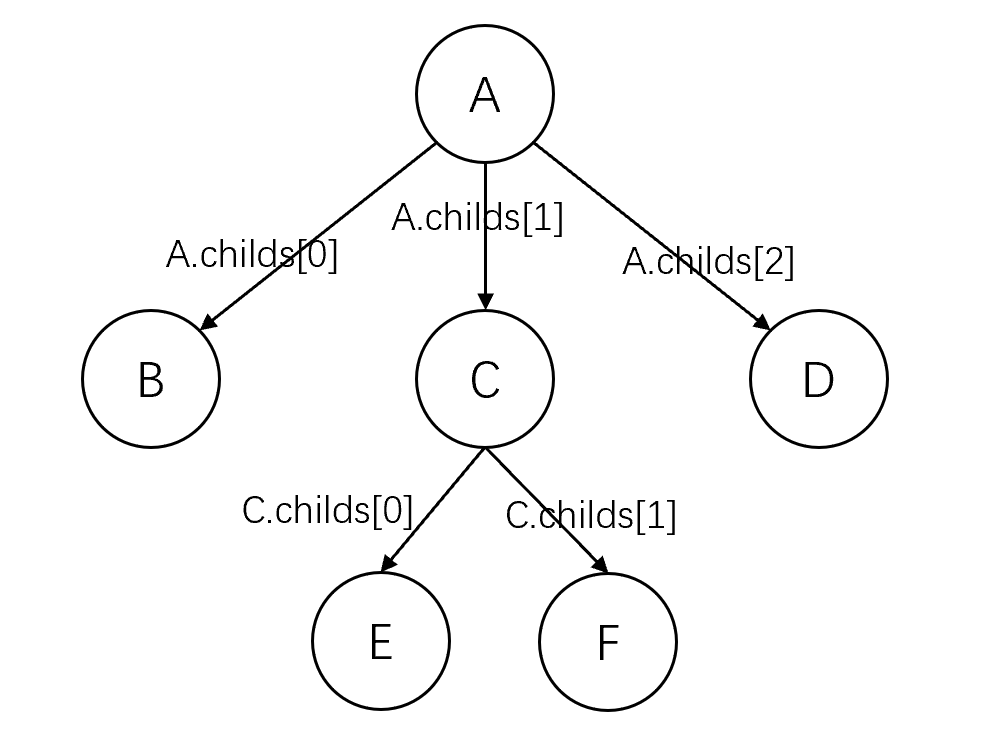
\includegraphics[width=0.47\textwidth]{assets/pics_and_ppts/ch4/树的不定长数组表示.png}
    \caption{用不定长数组表示树的孩子}
    \label{fig:用不定长数组表示树的孩子}
\end{figure}
这是完全可行，也非常自然的一种树的表示方式。但本书不要求大家熟悉C++，因此我们给出树的另一种表示方法，也是更高效的
\term{孩子-兄弟表示法（First Child - Next Sibling Representation）}。该方法存储每个节点的第一个孩子的指针，以及下一个兄弟的指针：
\begin{cppcode}
    struct TreeNode {
        ElemType data;
        TreeNode* first_child;
        TreeNode* next_sibling;
    };
\end{cppcode}
如图\ref{fig:树的孩子-兄弟表示法}所示。
\begin{figure}
    \centering
    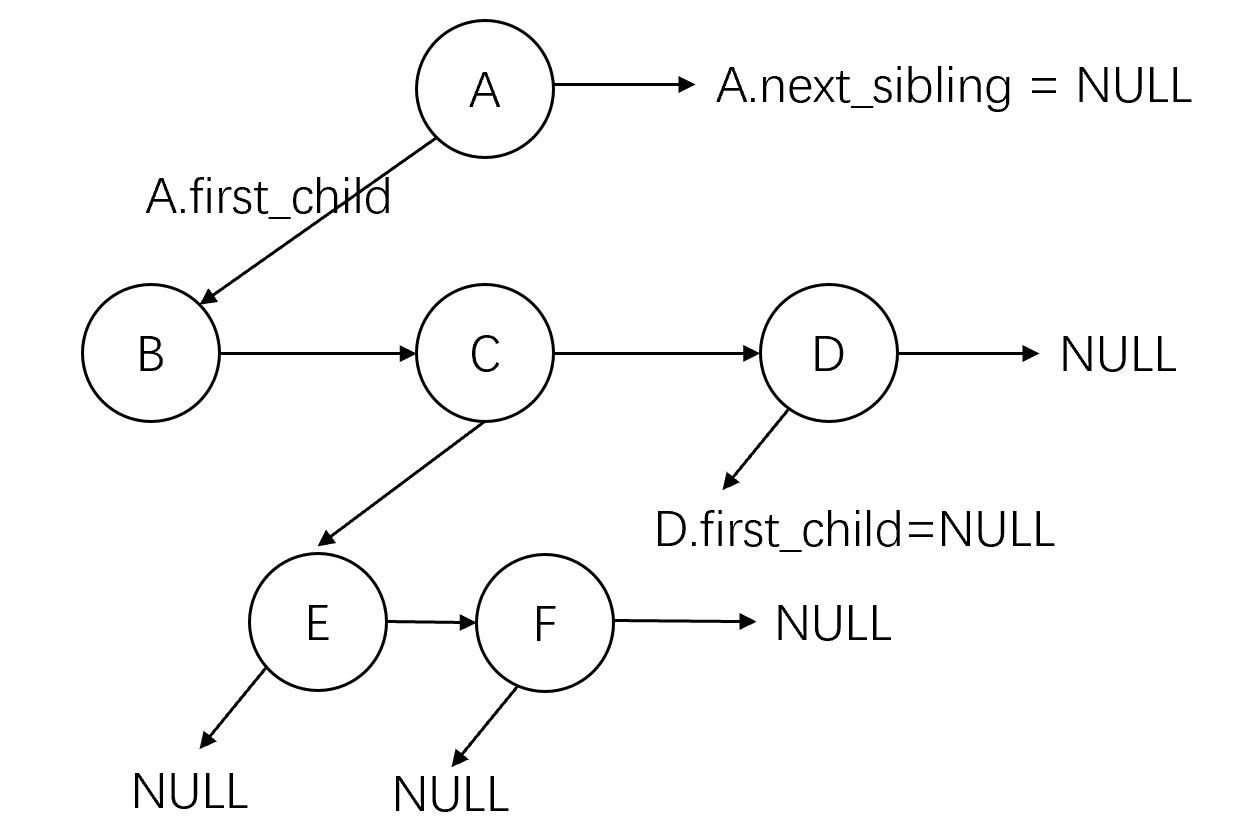
\includegraphics[width=0.6\textwidth]{assets/pics_and_ppts/ch4/树的孩子-兄弟表示法.png}
    \caption{树的孩子-兄弟表示法}
    \label{fig:树的孩子-兄弟表示法}
\end{figure}


显然该表示法下，只要拿到根节点指针，就能找到树中任何一个节点。因此，可以用根节点指针表示一棵树。如：
\begin{bulk}
    TreeNode* root; 
\end{bulk}
root这个对象既可以理解为树的根节点的指针，又可以理解为以root节点为根的一棵树。\\
\begin{notebox}{提示}
    图\ref{fig:用不定长数组表示树的孩子}与图\ref{fig:树的孩子-兄弟表示法}逻辑上是同一棵树，只不过物理指针的含义不同。
\end{notebox}


有了以上的内容介绍，我们来做一点有意思的事情（当然你大可以放心地跳过）：用孩子-兄弟表示法尝试实现操作系统的目录树。

\subsection{*目录树的简单实现}
我们已经知道，操作系统对目录的管理其实就是一棵树。用户随时可能在任何目录新建目录、删除某个目录，我们暂且不考虑文件。并假设目录节点的“数据”只有一个字符串
类型的成员，表示目录的名字，如“电影”等。以下代码实现了简单的新建目录、删除目录的操作，具体过程请结合注释。

\begin{cppcode}
    // 在目录Dad中，新建一个名为name的目录
    void DirInsert(TreeNode* Dad, char* name) {
        // 函数实现：创建一个新节点，将其加入Dad的孩子链表末尾
        TreeNode* new_node = (TreeNode*)malloc(sizeof(TreeNode));
        strcpy(new_node->name, name);
        new_node->first_child = NULL;
        new_node->next_sibling = NULL;

        // Dad原本是空目录，则需要更改first_child指针。
        if(Dad->first_child == NULL) {
            Dad->first_child = new_node;
            return;
        }

        // 原本不是空目录，修改next_sibling指针。
        TreeNode* last_child = Dad->first_child;
        while(last_child->next_sibling != NULL) {
            last_child = last_child->next_sibling;
        }
        last_child->next_sibling = new_node;
        return;
    }

    // 销毁一个节点及其所有后代
    void DestroyTree(TreeNode* root) {
        if(root == NULL) return;
        // 先递归销毁其子树
        DestroyTree(root->first_child);

        // 再释放根节点
        free(root);
    }

    // 在目录Dad中，删除目录to_del
    void DirDelete(TreeNode* Dad, TreeNode* to_del) {
        // 函数实现：先把to_del从父节点的孩子链表中摘掉，再销毁以to_del为根的整棵树
        if(Dad == NULL) {
            return;
        }
        // 要删除的就是第一个孩子节点，需要更新first_child指针
        if(to_del == Dad->first_child) {
            Dad->first_child = to_del->next_sibling;;
            // 注意这里不能简单地free(to_del)，因为该目录中可能还有若干目录，目录中可能还有目录，因此要递归销毁。
            DestroyTree(to_del);
            return;
        }

        // 找到要删除的节点的前一个兄弟节点
        TreeNode* pre = Dad->first_child;
        while(pre->next_sibling != to_del) {
            pre = pre->next_sibling;
        }

        // 修改链条，类似单链表的删除操作
        pre->next_sibling = to_del->next_sibling;
        // 注意同样要递归销毁
        DestroyTree(to_del);
        return;
    }
\end{cppcode}

\begin{notebox}{提示}
    以上例子也给了我们一个重要提示：树中每个节点的子节点很多时候不能单纯的看成一个节点，而是要看成一棵子树。因此与树相关的操作，很多都会涉及到递归，这一点非常重要。
\end{notebox}

\subsection{树的一些基本概念}
我们回到逻辑上的数据结构：树。树中有一些大家常用的专业术语与性质，我们在这里列出。\\
\begin{figure}
    \centering
    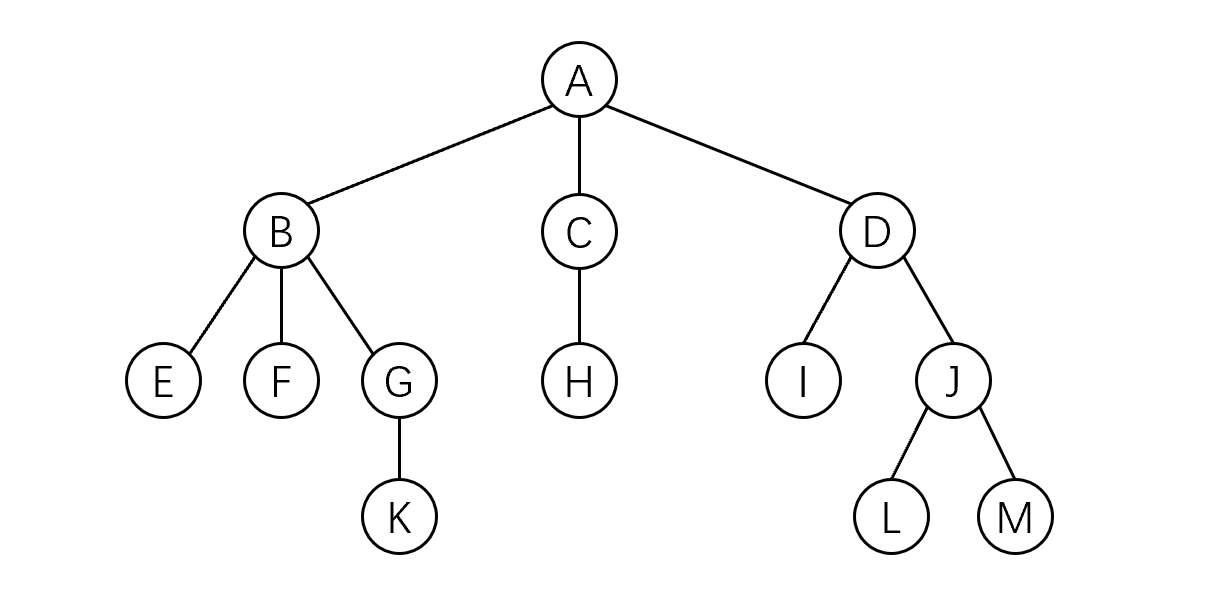
\includegraphics[width=0.6\textwidth]{assets/pics_and_ppts/ch4/一棵树.png}
    \caption{}
    \label{fig:一棵树}
\end{figure}

a）树中，一个节点拥有的子树数量称为\term{节点的度}。一棵树中所有节点的度的最大值称为这棵\term{树的度}。

b）树中度为0的节点称为\term{叶子节点}，简称\term{叶节点}。显然叶节点没有孩子节点。不是叶子节点的节点称为\term{非叶节点}。\\
图\ref{fig:一棵树}中，节点A、B的度均为3，整棵树的度为3；节点E、F、K、H、I、L、M的度为0，是叶子节点。\\
c）可以看出树是一种具有层次结构的数据结构。根节点处于最高层，通常定义根为第1层，根的孩子为第2层。若某节点处在第i层，其子树的根节点就处在第i+1层。

d）\term{节点的深度}通常定义为节点的所在层次；而\term{节点的高度}通常是指从最底层叶子节点（高度为1）开始逐层累加至该节点时的高度值。所有节点的深度
的最大值称为\term{树的深度}或\term{树的高度}。即
\begin{bulk}
    \begin{center}
        树的高度 = max\{所有节点的深度值\} = max\{所有节点的高度值\}
    \end{center}
\end{bulk}

图\ref{fig:一棵树}中，节点A的深度为1，高度为4；节点B的深度为2，高度为3；节点K的深度为4，高度为1。整棵树的深度，或称整棵树的高度，为4。

\begin{notebox}{提示}
    1.有些人喜欢将根节点的高度定义为0，本书若无特别说明，默认按照根节点高度为1来定义。\\
    2.注意区分节点与树的深度和高度：节点的高度和节点的深度通常不是一回事；而树的高度和树的深度一定是相等的。
\end{notebox}


\section{二叉树}
很少有实际问题需要直接通过二叉树来解决，但是二叉树在计算机科学中的应用是非常非常重要的。许多更加有用的数据结构都是一棵二叉树。而且对二叉树的研究可以为我们建立
类似树的层次结构的思维方式。笔者认为，对“二叉树”的研究在整个《数据结构》中都是相当重要的。
\begin{definitionbox}
    \term{二叉树}要么是一棵空树，要么是一棵：\\
    
    由根节点以及它的两棵子树构成的树，这两棵子树有左右位置之分，分别称为\term{左子树}和\term{右子树}，并且左子树和右子树依然是一棵二叉树。
\end{definitionbox}
可以看到，二叉树是\term{递归定义}的，即用二叉树自身来定义二叉树。
如图\ref{fig:几棵不同的二叉树}所示的几棵树都是二叉树，根据图中文字介绍，大家也能进一步体会二叉树的递归定义。
\begin{figure}
    \centering
    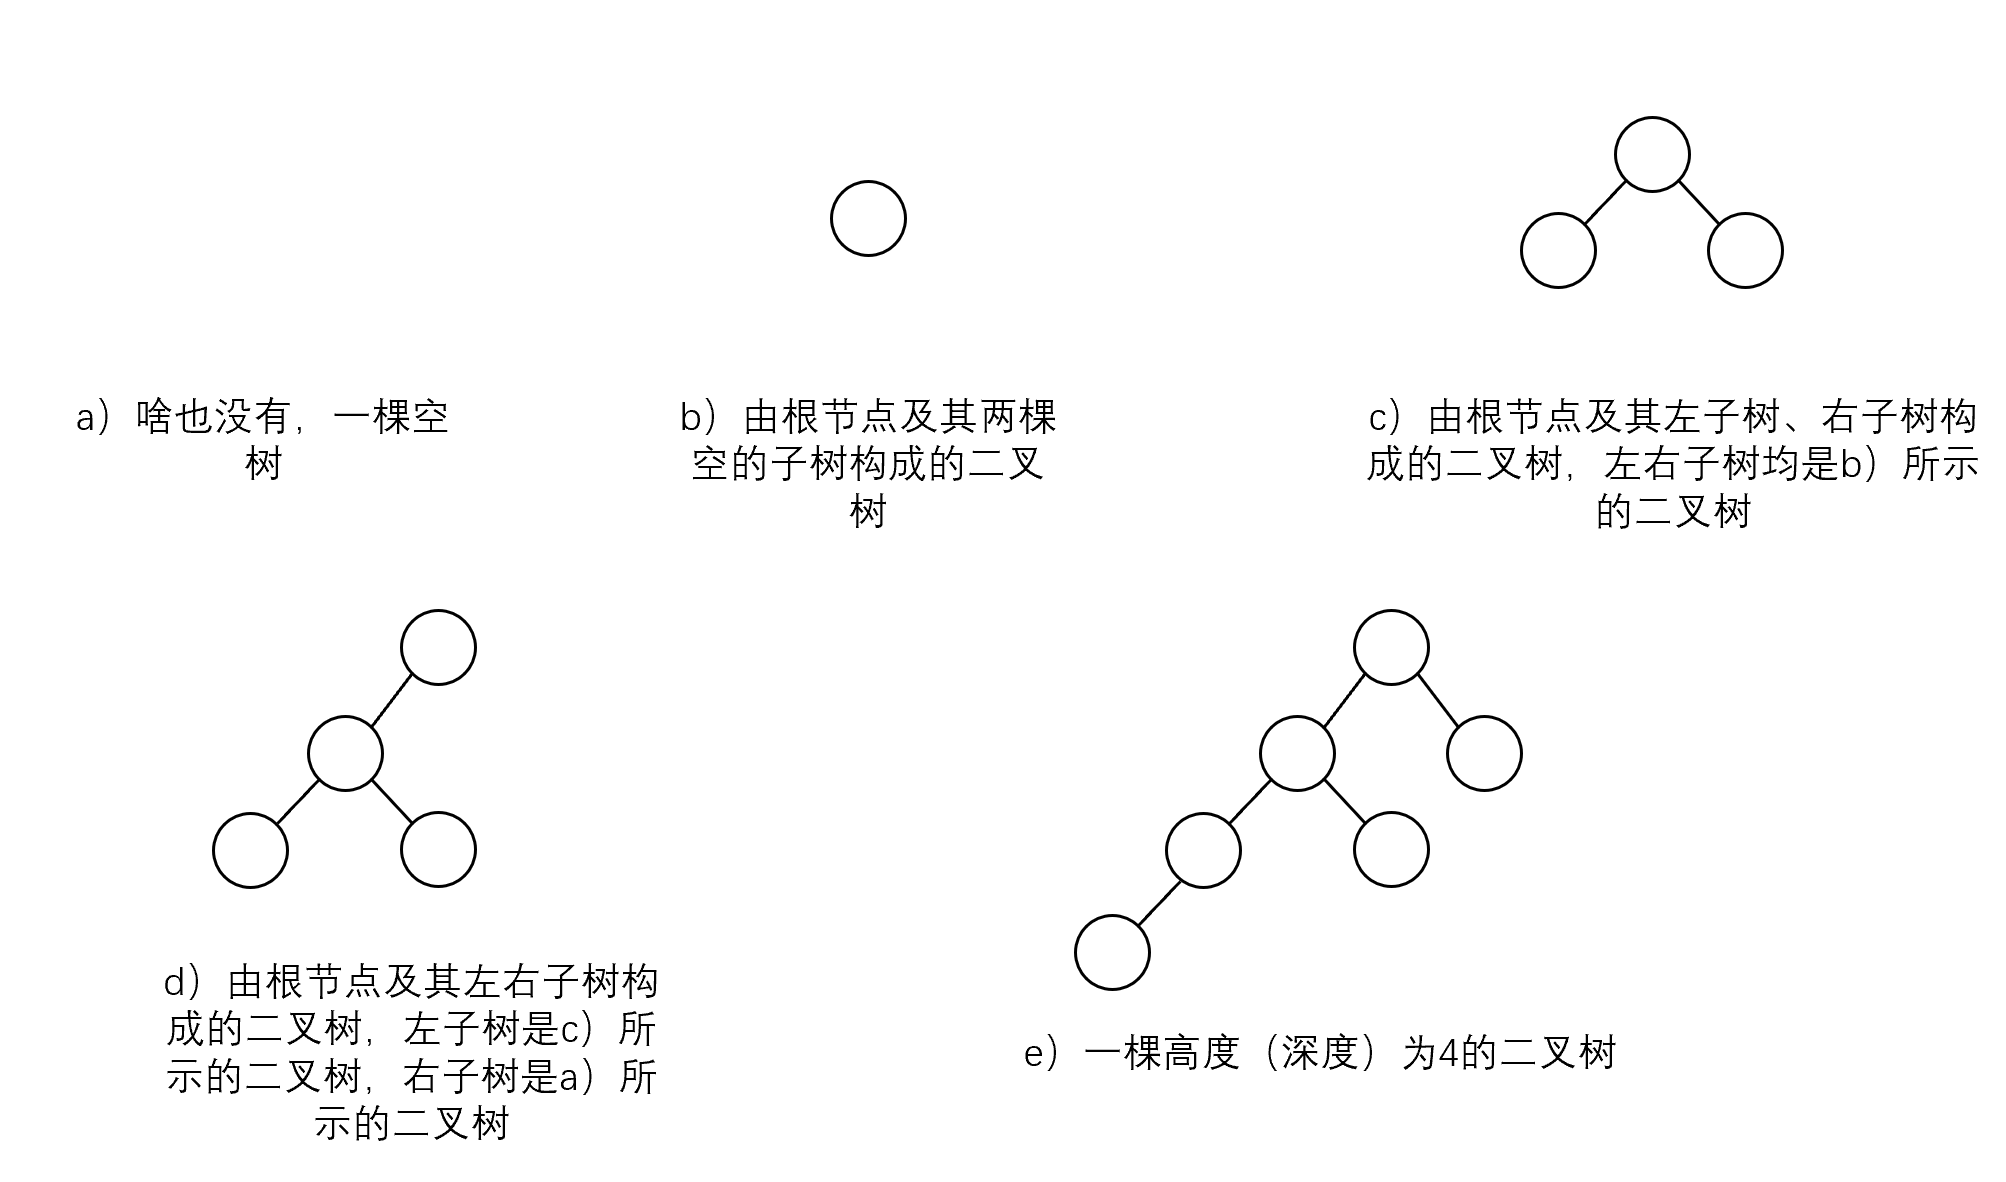
\includegraphics[width=1.0\textwidth]{assets/pics_and_ppts/ch4/几棵不同的二叉树.png}
    \caption{几棵不同的二叉树}
    \label{fig:几棵不同的二叉树}
\end{figure}

显然二叉树的度只可能是0、1或2，二叉树中每一个节点的度也只可能是0、1或2。



\begin{notebox}{提示}
    “二叉树”与“度为2的有序树”有如下区别：\\
    1. 度为2的树至少有3个节点，而二叉树未必；\\
    2. 二叉树即使只有一个孩子节点，该节点也要区分左右。而度为2的有序树，其“有序”是兄弟之间的位置有序，若某个节点是“独生子女”，则其位置是唯一确定的，不分左右。
    二叉树明确区分孩子的左右位置，这是因为在更多的场景下这是有用的，在后面的内容中我们将有所体会。
\end{notebox}



% 输出习题答案
\printanswers

\chapter*{--------- BONFIRE HIT ---------}

谢谢你带我来到这里，伴火同进者，终有一天会遇见命定之死，永别了。

\end{document}
